\documentclass[11pt]{book}
% Se imprime en papel de 80 gramos. Tapa blanda.
 
% Número de copias:
% 3 (para cada uno de los miembros del tribunal)
% 1 (para el lab)
% n (en versión gusanillo, para los evaluadores externos.
%    Por si lo piden)
% k (los que yo quiera. Sin abusar)

%%%%%%%%%%%%%%%%%%%%%%%%%%%%%%%%%%%%%%%%%%%%%%%%%%%%%%%%%%%%%%%%%%
%%                                                              %%
%%                           Packages                           %%
%%                                                              %%
%%%%%%%%%%%%%%%%%%%%%%%%%%%%%%%%%%%%%%%%%%%%%%%%%%%%%%%%%%%%%%%%%%

\usepackage[margin=2cm, paperwidth=17cm, paperheight=24cm, twoside]{geometry}
\usepackage{amsmath}
\usepackage{amsthm}
\usepackage{amssymb}
\usepackage{enumerate}
\usepackage{graphicx}
\usepackage{float}
\usepackage[sectionbib]{chapterbib}
\usepackage[font=small,labelfont=bf]{caption}
\usepackage{hyperref}
\usepackage{fancyhdr}
\usepackage{xcolor}
\usepackage{listings}
\usepackage{tikz}
\usepackage{adjustbox}

\newtheorem{theorem}{Theorem}

\lstdefinestyle{myStyle}{
  basicstyle=\tiny\ttfamily,           
  keywordstyle=\bfseries\color{blue},  
  commentstyle=\itshape\color{green},
  stringstyle=\color{orange},
  showstringspaces=false,
  breaklines=true,
  numbers=none,
  numberstyle=\tiny\color{gray},
  % A simple surrounding frame, or remove entirely:
  frame=none,
  % frame=single,
  rulecolor=\color{black},
  backgroundcolor=\color{white},
  tabsize=2,
  xleftmargin=1em,
  xrightmargin=1em
}
\lstset{style=myStyle}

\hypersetup{ 
    colorlinks=true,
    linkcolor=black,      
    urlcolor=blue,
    citecolor=black,
    pdftitle={Integrated multi-scale modeling for synthetic genetic constructions}
}

%%%%%%%%%%%%%%%%%%%%%%%%%%%%%%%%%%%%%%%%%%%%%%%%%%%%%%%%%%%%%%%%%%
%%                                                              %%
%%                           Preamble                           %%
%%                                                              %%
%%%%%%%%%%%%%%%%%%%%%%%%%%%%%%%%%%%%%%%%%%%%%%%%%%%%%%%%%%%%%%%%%%

\renewcommand{\bibname}{References}
\setcounter{tocdepth}{1}
\newcommand{\myfooter}{
    \ifodd\value{page} % Odd pages
        \ifnum\value{chapter}=0
            {\scriptsize\color{lightgray} \leftmark} %\relax % No chapter number if not defined
        \else
            \ifnum\value{chapter}=1
                {\scriptsize\color{lightgray} INTRODUCTION}
            \else
                {\scriptsize\color{lightgray} CHAPTER \thechapter}
            \fi
        \fi
    \else % Even pages
        {\scriptsize\color{lightgray} \rightmark}
    \fi
}
\fancypagestyle{plain}{
  \fancyhf{}
  \renewcommand{\headrulewidth}{0pt}
  \renewcommand{\footrulewidth}{0pt}
  \fancyfoot[C]{\myfooter}
  \fancyfoot[LE]{\thepage}
  \fancyfoot[RO]{\thepage}
}
\fancypagestyle{myobjectives}{
  \fancyhf{}
  \renewcommand{\headrulewidth}{0pt}
  \renewcommand{\footrulewidth}{0pt}
  \fancyfoot[C]{\scriptsize\color{lightgray} OBJECTIVES}
  \fancyfoot[LE]{\thepage}
  \fancyfoot[RO]{\thepage}
}
\fancypagestyle{myacknowledgements}{
  \fancyhf{}
  \renewcommand{\headrulewidth}{0pt}
  \renewcommand{\footrulewidth}{0pt}
  \fancyfoot[C]{\scriptsize\color{lightgray} ACKNOWLEDGEMENTS}
  \fancyfoot[LE]{\thepage}
  \fancyfoot[RO]{\thepage}
}
\fancypagestyle{almostempty}{
  \fancyhf{}
  \renewcommand{\headrulewidth}{0pt}
  \renewcommand{\footrulewidth}{0pt}
  \fancyfoot[LE]{\thepage}
  \fancyfoot[RO]{\thepage}
}
\pagestyle{plain}
\let\cleardoublepage\clearpage

\theoremstyle{definition}
\newtheorem{definition}{Definition}[section]
\newtheorem*{untheorem}{Theorem} 

% Prevent word splitting
\hyphenpenalty=10000
\exhyphenpenalty=10000
\sloppy

%%%%%%%%%%%%%%%%%%%%%%%%%%%%%%%%%%%%%%%%%%%%%%%%%%%%%%%%%%%%%%%%%%
%%                                                              %%
%%                  Title, Author and Advisors                  %%
%%                                                              %%
%%%%%%%%%%%%%%%%%%%%%%%%%%%%%%%%%%%%%%%%%%%%%%%%%%%%%%%%%%%%%%%%%%

\newcommand{\myself}{Lucas Goiriz Beltrán}

\title{
  \begin{center}
    % Logos row
    \vspace{-3cm}
    \begin{adjustbox}{center}
    \begin{tabular}{cccc}
        
\includegraphics[height=0.8cm]{assets/csic_logo.png} &
        
\includegraphics[height=1cm]{assets/i2sysbio_logo.png} &
        
\includegraphics[height=0.9cm]{assets/upv_logo.png} &
        
\includegraphics[height=1cm]{assets/dma_logo.jpg}
    \end{tabular}
    \end{adjustbox}
  
    \vspace{1cm}
  \end{center}
  \vspace{2cm}
  \makebox[\textwidth][c]{\rule{.9\textwidth}{2pt}}\\[1.2ex]
  \textbf{Stochastic dynamic modeling of evolving gene expression programs}\\[0.5ex]
  \makebox[\textwidth][c]{\rule{.9\textwidth}{2pt}}
}
\author{\textbf{Lucas GOIRIZ BELTRÁN}}
\date{
    \vfill
    \textbf{
        Thesis Advisors:\\
        Dr. Guillermo RODRIGO TÁRREGA\\
        Prof. Dr. J. Alberto CONEJERO CASARES
    }
    \vspace{1cm}
    \begin{center}
    Valencia, March 2025
    \end{center}
}

%%%%%%%%%%%%%%%%%%%%%%%%%%%%%%%%%%%%%%%%%%%%%%%%%%%%%%%%%%%%%%%%%%
%%                                                              %%
%%                           Document                           %%
%%                                                              %%
%%%%%%%%%%%%%%%%%%%%%%%%%%%%%%%%%%%%%%%%%%%%%%%%%%%%%%%%%%%%%%%%%%

\begin{document}
% Title page
\maketitle
\pagenumbering{gobble}
\pagebreak ~

% Dedication
\chapter*{}
\pagenumbering{roman}

\vspace*{1cm}
\begin{flushright}
\textit{Do not trust, verify ~~\\ ~ \\ --- vires in numeris ---}
\end{flushright}

% Abstracts
\chapter*{}
% English
\chapter*{\Large Stochastic dynamic modeling of evolving gene expression programs}

\vspace{-1cm}

\subsection*{\myself}

\subsection*{Abstract}
RNA viruses exemplify sophisticated genetic programs endowed with the capacity for change, offering a unique window into the interplay between intricate genomic design and dynamic potential. Building on a large-scale analysis of RNA virus genomic data, this work examines whether the accumulation of genetic modifications adheres to a constant-rate progression or exhibits more complex patterns. Central questions include how the distribution of genetic changes evolves over time, how distinct genetic profiles contribute to observed shifts, and whether these dynamics can be modeled by standard Poisson or Brownian processes. To address these questions, millions of publicly available sequences were processed, focusing on samples collected over an extended time period. Rigorous data filtering, multidimensional scaling, and temporal aggregation of mutational counts were employed to characterize both the mean and the variance in the number of substitutions relative to an early reference genome.

Findings reveal that while the average number of accumulated mutations increases linearly with time, variance in mutation counts follows a more intricate pattern than predicted by the classical molecular clock hypothesis. Specifically, marked accelerations of mutation rates occur when new variants, each carrying distinct genomic profiles, invade the population. Sub- or super-diffusive dynamics emerge in these variant-specific analyses, suggesting that the standard Brownian-motion model, commonly used to approximate neutral evolutionary processes, does not fully capture the underlying complexity. Instead, fractional Brownian motion with a time-dependent diffusion exponent better explains the observed discrepancies between mean and variance in mutation counts. This nuanced perspective is further supported by fluctuations in the ratio of nonsynonymous to synonymous substitutions (dN/dS), indicative of purifying selection with occasional adaptive events as new viral lineages spread.

Beyond refining long-standing molecular clock assumptions, this work contributes a novel analytical framework for understanding how population-wide dynamics, selection pressures, and transmission bottlenecks drive evolutionary trajectories in rapidly mutating RNA viruses. The integrative methodology, merging large-scale sequence data, variance-based metrics, and advanced modeling, can inform phylodynamic studies of other fast-evolving viruses. By exposing the limitations of purely Poissonian or Brownian models, these findings highlight the need for evolutionary frameworks that incorporate anomalous diffusion processes, profile-specific shifts in rate, and the broader ecological context of viral spread. Consequently, this work offers key insights into RNA virus evolution and underscores the importance of variance-based approaches in detecting critical deviations from conventional models, expanding our theoretical and practical understanding of viral adaptability and emergence.


\vfill

%%%%%%%%%%%%%%%%%%%%%%%%%%%%%%%%%%%%%%%%%%%%%%%%%%%%%%%%%%%%%%%%%%
% Spanish
\chapter*{\Large Modelado dinámico estocástico de programas de expresión génica evolutivos}

\vspace{-1cm}

\subsection*{\myself}

\subsection*{Resumen}
Los virus de ARN ejemplifican programas genéticos sofisticados dotados con capacidad de cambio, ofreciendo una ventana única a la interacción entre un intrincado diseño genómico y un potencial dinámico. Basándose en un análisis a gran escala de datos genómicos de virus de ARN, el presente trabajo examina si la acumulación de modificaciones genéticas se adhiere a una progresión de tasa constante o exhibe patrones más complejos. Las preguntas centrales incluyen cómo evoluciona la distribución de cambios genéticos a lo largo del tiempo, de qué manera perfiles genéticos distintos contribuyen a los cambios observados y si estas dinámicas pueden ser modeladas por procesos estándar de Poisson o Brownianos. Para abordar estas cuestiones, se procesaron millones de secuencias disponibles públicamente, concentrándose en muestras recolectadas durante un período temporal prolongado. Se aplicaron rigurosos filtros de datos, escalado multidimensional y agregación temporal de conteos mutacionales para caracterizar tanto la media como la varianza en el número de sustituciones con respecto a un genoma de referencia inicial.

Los hallazgos revelan que, mientras el número promedio de mutaciones acumuladas aumenta linealmente con el tiempo, la varianza en los conteos de mutaciones sigue un patrón más complejo del que predice la clásica hipótesis del reloj molecular. Específicamente, se observan aceleraciones marcadas en las tasas de mutación cuando nuevas variantes, cada una portadora de perfiles genómicos distintos, invaden la población. En estos análisis específicos de variantes emergen dinámicas sub- o super-difusivas, lo que sugiere que el modelo estándar de movimiento browniano, comúnmente utilizado para aproximar procesos evolutivos neutrales, no captura completamente la complejidad subyacente. En cambio, el movimiento fraccionario browniano con un exponente de difusión dependiente del tiempo explica de manera más adecuada las discrepancias observadas entre la media y la varianza en los conteos de mutaciones. Esta perspectiva matizada se ve respaldada además por las fluctuaciones en la proporción de sustituciones no sinónimas a sinónimas (dN/dS), indicativas de una selección purificadora con eventos adaptativos ocasionales a medida que se diseminan nuevas líneas virales.

Más allá de refinar las antiguas suposiciones del reloj molecular, este trabajo contribuye con un novedoso marco analítico para comprender cómo las dinámicas a nivel poblacional, las presiones selectivas y los cuellos de botella en la transmisión impulsan las trayectorias evolutivas en virus de ARN de rápida mutación. La metodología integradora, que fusiona datos de secuencias a gran escala, métricas basadas en la varianza y modelos avanzados, puede orientar estudios filodinámicos de otros virus de evolución acelerada. Al exponer las limitaciones de los modelos puramente Poissonianos o Brownianos, estos hallazgos resaltan la necesidad de marcos evolutivos que incorporen procesos de difusión anómala, cambios específicos en la tasa según el perfil y el contexto ecológico más amplio de la propagación viral. En consecuencia, el presente trabajo ofrece importantes aportes sobre la evolución de los virus de ARN y subraya la relevancia de los enfoques basados en la varianza para detectar desviaciones críticas de los modelos convencionales, ampliando así nuestra comprensión teórica y práctica de la adaptabilidad y emergencia viral.

\vfill

%%%%%%%%%%%%%%%%%%%%%%%%%%%%%%%%%%%%%%%%%%%%%%%%%%%%%%%%%%%%%%%%%%
% Valencian
\chapter*{\Large Modelatge dinàmic estocàstic de programes d'expressió gènica evolutius}

\vspace{-1cm}

\subsection*{\myself}

\subsection*{Resum}
Els virus d'ARN exemplifiquen programes genètics sofisticats dotats de la capacitat de canviar, oferint una finestra única sobre la interacció entre un disseny genòmic complex i un potencial dinàmic. Basant-se en una anàlisi a gran escala de dades genòmiques de virus d'ARN, aquest treball examina si l'acumulació de modificacions genètiques s'ajusta a una progressió de taxa constant o bé manifesta patrons més complexos. Les qüestions centrals inclouen com evoluciona la distribució dels canvis genètics al llarg del temps, com els diferents perfils genètics contribueixen als desplaçaments observats i si aquestes dinàmiques poden ser modelades per processos de Poisson o de Brown estàndard. Per abordar aquestes qüestions, es van processar milions de seqüències d'accés públic, amb un focus especial en les mostres recollides durant un període de temps prolongat. Es va dur a terme una rigorosa depuració de dades, escalat multidimensional i agregació temporal dels comptes de mutacions per caracteritzar tant la mitjana com la variància en el nombre de substitucions respecte a un genoma de referència inicial.

Els resultats revelen que, tot i que el nombre mitjà de mutacions acumulades augmenta de manera lineal amb el temps, la variància en els comptes de mutacions segueix un patró més intricada del que prediu la hipòtesi clàssica del rellotge molecular. Concretament, s'observen acceleracions marcades de les taxes de mutació quan noves variants, cadascuna amb perfils genòmics distintius, invadeixen la població. Dins d'aquestes anàlisis específiques per variant emergeixen dinàmiques sub- o super-difusives, la qual cosa suggereix que el model de moviment brownià estàndard, comunament utilitzat per aproximar processos evolutius neutres, no capta completament la complexitat subjacent. En lloc d'això, el moviment fraccionari brownià amb un exponent de difusió dependent del temps explica millor les discrepàncies observades entre la mitjana i la variància dels comptes de mutacions. Aquesta perspectiva matisada es veu reforçada per les fluctuacions en la relació de substitucions nonsinònimes a sinònimes (dN/dS), indicatives d'una selecció purificadora amb esdeveniments adaptatius ocasionals a mesura que es difonen noves línies vírals.

Més enllà de refinar les assumpcions del rellotge molecular de llarga data, aquest treball aporta un nou marc analític per entendre com les dinàmiques a nivell poblacional, les pressions selectives i els colls de botella en la transmissió impulsen les trajectòries evolutives en virus d'ARN que muten ràpidament. La metodologia integradora, que fusiona dades de seqüències a gran escala, mètriques basades en la variància i modelatge avançat, pot informar estudis filodinàmics d'altres virus d'alta evolució. En exposar les limitacions dels models purament poissonians o brownians, aquests resultats destaquen la necessitat de marcs evolutius que incorporen processos de difusió anòmala, canvis en la taxa específics de cada perfil i el context ecològic més ampli de la propagació viral. En conseqüència, la recerca ofereix coneixements clau sobre l'evolució dels virus d'ARN i subratlla la importància d'enfocs basats en la variància per detectar desviacions crítiques dels models convencionals, ampliant finalment la nostra comprensió teòrica i pràctica de l'adaptabilitat i l'aparició de nous virus.


\vfill

% Contents
\chapter*{}
\tableofcontents
\vfill
\pagebreak
\thispagestyle{almostempty}


\pagestyle{plain}
\pagenumbering{arabic}
\chapter{Introduction}
\begin{flushright}
    \textit{Above all, my life is research.}\\
    --- Margarita Salas
\end{flushright}

\vspace{1cm}

\section{Mathematical Modeling in Biology}
%\subsection{Overview of Mathematical Modeling in Biological Sciences}
Biological systems are extraordinarily complex, involving multifaceted interactions that span from molecules to entire ecosystems. Because traditional experimental approaches often cannot fully capture this complexity, mathematical modeling has become an indispensable tool for biologists to understand, simplify, and predict system behaviors. These models provide a structured framework for analyzing biological processes, generating hypotheses, and integrating experimental data into a coherent representation of larger systems. By offering quantitative predictions, mathematical models enable the testing of hypotheses under controlled \textit{in silico} conditions, thereby uncovering insights that might be challenging to observe directly \cite{banwarth-kuhn2020how}. Indeed, many recent biological breakthroughs are rooted in the synergy between modeling, experimental observation, and hypothesis testing \cite{servedio2014not}. Although models focus on essential features of a system to clarify underlying principles, they rely on assumptions and simplifications that can produce inaccuracies if chosen poorly \cite{brown2018evaluating}. Thus, iterative model refinement and experimental validation are vital to ensure that each model accurately represents the biological phenomenon under study.

% \subsection{Applications in Gene Regulation} \textbf{Applications in Gene Regulation.}
Mathematical modeling has had a profound impact on deciphering gene regulation, where it has become essential for unraveling the complex mechanisms of transcriptional control and gene expression. Gene regulation involves a network of interactions between transcription factors, DNA, RNA, and other cellular components, collectively determining whether a gene is activated or silenced. The emergence of high-throughput genomic technologies in the early 21$^\text{st}$ century generated a substantial amount of data, spurring new advances in modeling \cite{ay2011mathematical}. Modeling is especially important in this context because gene expression lies at the intersection of numerous biological processes; even subtle changes in regulatory interactions can drive diseases, phenotypic variation, or evolutionary novelties \cite{ay2011mathematical}. By offering a quantitative framework, mathematical models simulate regulatory networks and predict how modifications in specific components influence overall gene expression \cite{banwarth-kuhn2020how}. These models also clarify how gene expression is coordinated from the single-cell level to entire organisms, yielding a deeper comprehension of development and cellular function. A noteworthy illustration involves modeling gene regulation in early \textit{Drosophila melanogaster} embryogenesis, where spatial expression patterns are explained by reaction-diffusion principles that identify critical interactions \cite{reinitz-sharp1995mechanism, jaeger-surkova2004dynamicControl, jaeger-surkova2004dynamicAnalysis}. In synthetic biology, mathematical models guide the design of gene circuits that exhibit oscillations \cite{elowitz2000synthetic} or switch-like behaviors \cite{gardner-cantor2000}, demonstrating the broad applications of these approaches.

%\subsection{Applications in Epidemiology} \textbf{Applications in Epidemiology.}
In epidemiology, mathematical models are instrumental in studying the spread of infectious diseases and assessing the effectiveness of diverse public health interventions \cite{siettos2013mathematical}. By simulating disease transmission within populations, these models predict outbreaks, gauge the potential outcomes of vaccination strategies, and evaluate containment measures. Over the past few decades, they have become an essential component of public health policy making \cite{temime2008rising, miguelAngel2021}, proving indispensable during crises such as the 2014 Ebola outbreak in West Africa and the recent COVID-19 pandemic. By forecasting disease trajectories, modeling aids both immediate and longer-term policy decisions, including social distancing mandates and lockdown protocols. As infectious diseases continue to present urgent challenges, epidemiological modeling will remain a key instrument for understanding disease dynamics and guiding public health responses \cite{siettos2013mathematical}.

%\subsection{Applications in Evolutionary Biology} \textbf{Applications in Evolutionary Biology.}
Mathematical modeling has had also a long and influential history in evolutionary biology, where it has been essential for elucidating the mechanisms that govern genetic change. In particular, these models help address questions that are experimentally challenging due to the long timescales characterizing evolutionary processes \cite{brown2018evaluating}. They enable the exploration of natural selection, genetic drift, mutation, and migration, all of which collectively determine how genetic variation changes in populations over generations \cite{johri-aquadro2022recommendations,rosenberg-stadler-steel2025aMathematical}. By incorporating quantitative equations into evolutionary theory, researchers can predict genetic trends, evaluate the forces that drive evolution, and examine the coevolution of species or the emergence of advantageous mutations \cite{servedio2014not}. Such modeling further allows the testing of theoretical ideas about evolutionary processes, providing insights into species origins and adaptations that guide future research directions in evolutionary biology. To delve more deeply into how these processes unfold over time, it is crucial to understand evolution as a stochastic phenomenon, where random events play a significant role in shaping genetic outcomes.

\section{Evolution as a Stochastic Process}
Evolution proceeds through four fundamental processes: mutation, natural selection, genetic drift, and recombination, each of which has an inherent random component that lends itself to stochastic models \cite{Arenas2015, siepel2009}. Mutation introduces new variants at rates typically modeled by Poisson processes, whereas selection favors or disfavors certain variants based on fitness effects. Drift acts as a random sampling event that can fix or eliminate alleles regardless of fitness, especially in small populations, while recombination reorganizes genetic material to produce new haplotype combinations.

Markov models frequently capture these processes by assigning\linebreak state-dependent transition rates for sequence changes, and continuous-time Markov chains (CTMCs), for instance, quantify the instantaneous substitution rates among nucleotides or amino acids. Traditionally, these models have been used to describe the evolution of DNA sequences. Formally, a Markov chain is a stochastic process $\{X_t, t \geq 0\}$ characterized by the Markov property, which states:

\begin{equation}
P(X_{t+s} = j \mid X_t = i, X_u = x_u, u < t) = P(X_{t+s} = j \mid X_t = i)
\end{equation}
for all states $i, j$ and times $t, s \geq 0$. The process is fully described by its transition probabilities $P_{ij}(t) = P(X_{t+s}=j \mid X_s=i)$, which satisfy the Chapman-Kolmogorov equations:

\begin{equation}
P_{ij}(t+s) = \sum_{k} P_{ik}(t) P_{kj}(s), \quad \text{for all } t,s \geq 0.
\end{equation}

In a continuous-time context, transitions occur according to rates defined by a rate matrix $Q = \{q_{ij}\}$, where each off-diagonal entry $q_{ij}$ represents the instantaneous rate of moving from state $i$ to state $j$, and diagonal entries are defined such that $q_{ii} = -\sum_{j \neq i} q_{ij}$. Thus, the transition probability matrix over time $t$ can be computed through matrix exponentiation:

\begin{equation}
P(t) = e^{Qt}.
\end{equation}

To integrate Markov chains into the evolutionary model, we consider the following explanatory scheme:

\begin{enumerate}
    \item \textbf{State Definition}: Define each state of the Markov chain to represent a particular genetic configuration or nucleotide/amino acid sequence.
    \item \textbf{Transition Rates}: Specify transition rates $q_{ij}$ based on biological mechanisms such as mutation rates, selection coefficients, and drift probabilities.
    \item \textbf{Rate Matrix Construction}: Assemble the rate matrix $Q$ encapsulating all possible instantaneous transitions between genetic states.
    \item \textbf{Transition Probabilities Calculation}: Calculate transition probability matrices $P(t)$ using matrix exponentiation to predict evolutionary dynamics over time.
    \item \textbf{Integration into Phylogenetic or Population Genetic Models}: Employ these computed transition probabilities in models such as Wright-Fisher, Moran, or phylogenetic inference frameworks to estimate divergence times, genetic variability, or ancestral states.
\end{enumerate}

Although Markov models are powerful tools for describing evolutionary processes, their simplest forms make assumptions about rate homogeneity across time and states, and may fail to capture the full complexity of biological systems. For instance, as multiple generations pass, deterministic selection interacts with stochastic mutation and drift, resulting in intricate patterns of divergence. Models such as Wright-Fisher and Moran (including diffusion and coalescent extensions) offer a theoretical foundation for quantifying these random dynamics \cite{griffiths-marjoram1996}. Consequently, beneficial mutations can still be lost if chance events override selection in finite populations \cite{haldane1937effect}, illustrating how randomness profoundly influences molecular evolution.

Population genetics predominantly examines allele frequency changes within species, relying on models like Wright-Fisher or coalescent theory to incorporate drift, selection, and mutation in a finite population \cite{hein2004gene}. By tracking the probabilities of fixation or loss over discrete generations, population-genetic analyses elucidate microevolutionary dynamics, including the relative roles of neutrality and adaptation. Phylogenetics, conversely, focuses on substitutions that accumulate between diverging lineages, often modeling sequence evolution with continuous-time Markov chains along the branches of a tree. Here, each branch length reflects the expected number of substitutions per site, and likelihood-based or Bayesian methods assess different phylogenetic hypotheses \cite{KosiolGoldman2011}. Although both fields consider the same fundamental processes, they differ in timescale and scope: population genetics addresses polymorphisms within populations, while phylogenetics assumes fixed differences between species. Furthermore, recombination complicates phylogenetic inference by creating discordant gene trees, whereas in population genetics it may accelerate adaptation or break up linkage. Recent methodological advances bridge these perspectives, for instance by integrating coalescent theory into species-tree approaches that accommodate incomplete lineage sorting. Ultimately, both population genetics and phylogenetics leverage stochastic models to reconstruct evolutionary history, yet they do so with distinct focuses on the micro versus macro dimensions of biological change. To date, the two fields are complementary and not in competition. A core framework for both fields involves the molecular clock, which uses evolutionary rates to date divergence times across lineages.


\section{The Concept of the Molecular Clock}
The molecular clock hypothesis traces back to the 1960s when Zuckerkandl and Pauling observed a roughly consistent rate of molecular changes and proposed that these changes could be treated as a ``clock'' for dating evolutionary events \cite{zuckerkandl-pauling1965}. Kimura's Neutral Theory later provided theoretical support by suggesting that the majority of substitutions are selectively neutral and accumulate at a near-constant rate through genetic drift \cite{Bromham2003}. Early strict clock models treated substitutions as a Poisson process with a uniform rate across all lineages \cite{takahata2007}, but empirical evidence often contradicted this rigidity. Consequently, relaxed clocks were introduced to permit variable substitution rates across branches within a statistically coherent framework \cite{Drummond2006}. 

In a strict molecular clock framework, the accumulation of substitutions is modeled by a Poisson process. Let $N(t)$ denote the number of substitutions that occur along a lineage during a time interval $t$. Assuming a constant substitution rate $\mu$ (substitutions per unit time), the probability that exactly $k$ substitutions occur in time $t$ is given by the Poisson probability mass function:
$$
P\left(N(t) = k\right) = \frac{(\mu t)^k e^{-\mu t}}{k!}, \quad k = 0, 1, 2, \dots
$$
Here, the expected number of substitutions is
$$
\mathbb{E}[N(t)] = \mu t,
$$
and due to the properties of the Poisson distribution, the variance is also
$$
\mathbb{V}(N(t)) = \mu t.
$$
This formulation encapsulates the idea that both the mean and the variance of the substitution process increase linearly with time. However, empirical studies have noted that observed variance often exceeds the mean (overdispersion), suggesting that factors such as lineage-specific rate heterogeneity, episodic selection, and other evolutionary forces may cause deviations from the strict Poisson assumption \cite{Gillespie1984, Ho2011}. Such observations have motivated the development of relaxed clock models, which allow for rate variation among lineages while maintaining a statistically coherent framework for divergence time estimation.

Estimating these rates and divergence times typically employs likelihood or Bayesian methods, with Bayesian approaches (including MCMC in BEAST) yielding comprehensive posterior distributions of tree topology, rates, and node ages \cite{Kumar2016}. Nonetheless, current models exhibit inherent limitations: lineage rate heterogeneity can induce overdispersion \cite{Gillespie1984}, while temporal rate shifts complicate calibrations that presume uniformity \cite{Ho2011}. External factors, episodic selection, and calibration errors further exacerbate these biases, stressing the importance of careful model selection, robust calibrations, and thorough statistical analyses. To address these challenges, refined techniques such as penalized likelihood, correlated and uncorrelated relaxed clocks, life-history trait covariates, and partitioned models for distinct genes have been developed. Although these approaches mitigate biases, they can be computationally demanding when handling extensive datasets. Despite these hurdles, the molecular clock remains invaluable for reconstructing deep evolutionary timelines and guiding phylodynamic studies of fast-evolving pathogens, highlighting both its enduring utility and the necessity for ongoing methodological improvements. In many instances, studies of RNA viruses offer particularly clear examples of these principles.


\section{Viruses as complex gene expression programs: RNA viruses as a case study}
RNA viruses exhibit exceptionally high mutation rates and rapid replication dynamics that render them ideal models for testing molecular clock hypotheses. A virus's genomic architecture is composed of multiple genes, many of which are multifunctional, that form a complex regulatory circuit with numerous interactions with the host cell. In combination with their intricate regulatory circuitry, these mutations set the stage for swift evolutionary divergence. Moreover, their short generation times and large population sizes further facilitate measurable divergence, producing a clear temporal signal in their genome sequences \cite{Holmes2009}. Consequently, RNA viruses are classified as `measurably evolving populations'', where genetic divergence correlates directly with elapsed time, enabling precise calibration of molecular clocks \cite{Grenfell2004}. This real-time evolution provides a natural laboratory for studying substitution rate variability, selective pressures, and the underlying dynamics of sequence evolution. As such, researchers can rigorously test and refine theoretical models by directly observing evolutionary processes over short time scales, thereby bridging theoretical frameworks with empirical data. Continuous monitoring of viral genomes not only validates molecular clock assumptions but also enhances our understanding of broader evolutionary and epidemiological phenomena, underscoring the critical role these viruses play in advancing molecular evolutionary research.

In the realm of public health, RNA viruses represent significant threats due to their rapid evolution and widespread transmission, as exemplified by the ongoing SARS-CoV-2 pandemic. High-throughput sequencing technologies have revolutionized viral surveillance by enabling rapid, cost-effective sequencing of whole genomes directly from clinical samples. This surge in genomic data empowers researchers to perform time-resolved phylogenetic analyses and robust mathematical modeling, which are crucial for understanding transmission dynamics and predicting epidemic trends \cite{Grubaugh2019, Pollett2020}. Phylodynamic approaches integrate evolutionary data to infer key epidemiological parameters such as outbreak origins, transmission rates, and timing of introductions. These models have been instrumental in guiding interventions, ranging from travel restrictions and quarantine measures to vaccine deployment strategies. Specifically, SARS-CoV-2 has been extensively monitored using millions of genome sequences, allowing scientists to track the emergence and spread of variants in near real-time. The integration of genomic and epidemiological metadata further enhances forecasting capabilities, ensuring that public health responses are both timely and data-driven \cite{Hill2021, Gire2014, Luksza2014}.


\section{Research Gaps and Motivation}
Despite significant advances, evolutionary models remain limited by simplifying assumptions that may not fully capture complex biological realities. Classical models often assume independent loci, constant selection pressures, or simplified recombination dynamics, yet empirical studies reveal pervasive epistasis, variable selection, and linkage effects that challenge these assumptions \cite{lunzer2010pervasive, neher2009competition}. Refining models to incorporate these factors requires a balance between mathematical tractability and biological realism. Recent approaches leverage stochastic processes, Bayesian inference, and simulation-based methods to enhance predictive accuracy \cite{csillery2010approximate, meyer2017accelerating}. However, the stochastic frameworks employed in these models typically incorporate white noise, Gaussian delta-correlated fluctuations, due to its mathematical convenience. While this choice has facilitated substantial advances, it may not capture the full complexity of biological systems. There is growing reason to believe that alternative, more intricate noise models could more accurately represent the stochasticity inherent in evolutionary processes. Furthermore, computational demands grow exponentially, necessitating efficient algorithms and scalable implementations.


Addressing these challenges requires an interdisciplinary approach that integrates evolutionary theory, applied mathematics, and computer science. Advances in Monte Carlo simulations, machine learning, and high-performance computing now enable inference of complex models, but accessibility remains a concern \cite{bryant2017special}. Open-source software plays a pivotal role in democratizing these tools, ensuring reproducibility and fostering collaboration \cite{bouckaert2014beast, haller2019slim}. Platforms such as BEAST, SLiM, and Approximate Bayesian Computation (ABC) frameworks exemplify how theoretical models can be practically implemented for real-world data analysis. The ongoing challenge lies in developing flexible, scalable, and biologically realistic models that bridge theoretical derivations with empirical data, ultimately refining our understanding of molecular evolution.

\bibliographystyle{assets/rodrigostyle}
\bibliography{references/introductionReferences}

\vfill
\pagebreak
\newpage ~

\chapter{Objectives}
\thispagestyle{myobjectives}

The evolutionary dynamics of rapidly mutating biological systems involve complex interactions between localized genetic events and broader population-level outcomes, resulting in behaviors that are not well-captured by classical evolutionary models. Quantifying these processes necessitates robust modeling frameworks, a detailed understanding of gene-level heterogeneity, and scalable analytical methods. Therefore, this thesis has the following objectives:

\begin{enumerate}
    \item Investigate the underlying stochastic processes and localized mutation dynamics in rapidly mutating biological systems, assessing how these micro-level events collectively influence macroscale evolutionary outcomes.
    \item Evaluate selective pressures across diverse genomic segments and identify deviations from classical evolutionary models by employing alternative quantitative frameworks to elucidate patterns of adaptation and constraint.
    \item Verify whether the molecular clock hypothesis holds in rapidly mutating biological systems or if significant deviations arise due to localized genetic variability.
    \item Develop and implement integrated computational and statistical methodologies, coupled with novel large-scale open-source data treatment approaches, to bridge localized evolutionary events with comprehensive genomic-scale dynamics while ensuring reproducibility and scalability.
\end{enumerate}

\pagestyle{plain}
\vfill
\pagebreak ~


\chapter{A variant-dependent molecular clock with anomalous diffusion models SARS-CoV-2 evolution in humans}\label{ch:chapter2}

%% TODO:
% - Completar com más info donde esté marcado con "%%%"

\begin{flushright}
    \textit{Simplicity is prerequisite for reliability.}\\
    --- Edsger W. Dijkstra
\end{flushright}

\vspace{1cm}

\noindent This work has been published in a peer-reviewed journal. See the full citation:\\

\noindent \textbf{Goiriz L}, Ruiz R, Garibo-i-Orts O, Conejero J.A, Rodrigo G. (2023) \href{https://doi.org/10.1073/pnas.2303578120}{A variant-dependent molecular clock with anomalous diffusion models SARS-CoV-2 evolution in humans}. \textit{Proc. Natl. Acad. Sci. U.S.A.}, 120(30): e2303578120.\\

\noindent In this publication, I performed all the data analysis and figures, except for \textbf{Figure \ref{fig:fig2.2}} where OGO made contributions in the data analysis. The results were discussed with RR, JAC and GR. GR designed the research.

\vfill

\pagebreak

\sloppy

\section{Introduction}

Viruses lie at the frontier of living and inert matter, as they lack own metabolism to sustain replication but are subject to Darwinian evolution (\textit{i.e.}, mutation and selection) \cite{koonin2013}. As fast evolving biological agents \cite{drake1998}, they are ideal substrates from which to learn mechanisms that modulate genetic variation, as well as to test theoretical models of evolution. One important model is the molecular clock hypothesis, introduced by Emile Zuckerkandl and Linus
Pauling, which dates back to early times of molecular biology.

\begin{definition}[Molecular Clock Hypothesis (1965)]
    The molecular clock hypothesis states that the rate of evolution of a gene is constant over time. This implies that genes accumulate mutations at a constant rate, providing a molecular basis for measuring evolutionary timescales \cite{zuckerkandl1965,ayala1999,kumar2005}.
\end{definition}

Motoo Kimura further developed this theory into a comprehensive framework in known as the neutral theory of molecular evolution.

\begin{definition}[Neutral Theory of Molecular Evolution (1968)]
    The neutral theory of molecular evolution proposes that most evolutionary changes at the molecular level are caused by random genetic drift of selectively neutral mutants \cite{kimura1968,kimura1987}.
\end{definition}

Neutral theory of molecular evolution predicts, in addition, that such clocks are Poissonian stochastic processes (\textit{i.e.}, evolution seen as a Brownian motion with diffusivity such that mean and variance are equal) \cite{kimura1987}, a concept that will be elaborated upon in \textbf{Section \ref{sec:evolution-approximated-as-a-continuous-stochastic-process}}. Despite the results from seminal studies of some viral genes are in tune \cite{gojobori1990,leitner1999}, the molecular clock hypothesis still raises controversy \cite{kumar2005}, as evolution appears as a highly volatile and vagary stochastic process due to environmental changes, transmission bottlenecks, and recombination and speciation events. Indeed, such a null model can be rejected in numerous cases \cite{jenkins2002}, and overdispersed populations in genetic variation (\textit{i.e.}, with larger variance than mean) seem common across phyla \cite{bedford2008}. Nonetheless, without extensive monitoring of evolution in natural conditions for a reasonable period of time, it is difficult to describe the mathematical model underlying such stochastic dynamics.

The emergence (at the end of 2019) and global spread (during 2020) of severe acute respiratory syndrome coronavirus 2 (SARS-CoV-2) has caused the ongoing pandemic \cite{li2021}. Due to the high impact on public health, huge efforts have been carried out worldwide to sequence the whole viral genome from different patients in real time of pandemic \cite{bedford2020, lopez2021, lemieux2021, tegally2021, kraemer2021, rockett2022, jackson2021}. To date, more than 10 million sequences are available. Importantly, this has allowed tracking introductions and measuring the extent of virus transmission at the community level \cite{bedford2020}, assessing the effectiveness of containment strategies \cite{lopez2021}, realizing the impact of superspreading events \cite{lemieux2021}, identifying novel variants of concern and their key mutations \cite{tegally2021}, monitoring spatiotemporal invasion dynamics of specific variants \cite{kraemer2021}, disclosing co-infection occurrences with different variants \cite{rockett2022}, and discovering the circulation of recombinant viruses, which might lead to increased infectiousness or pathogenicity \cite{jackson2021}. In addition, computational analyses have shown that SARS-CoV-2 primary evolves under purifying selection in humans, with some sites displaying adaptation \cite{rochman2021}. They have also shown that the spectrum of acquired mutations is greatly asymmetric (\textit{viz.}, dominated by C$>$U and G$>$U substitutions) \cite{yi2021}. Notwithstanding, a detailed study of the stochastic dynamics underlying such evolutionary motion to assess fundamental scaling laws and conditions for criticality has not been carried out.

In this work, we exploited the unprecedented monitoring of the evolution of a human virus in nature to conduct a study aimed at describing this process as a (non-)Brownian motion, considering the number of acquired mutations as the displacement of the viral particle from the origin (\textbf{Fig. \ref{fig:fig2.1}}). For that, several biostatistical analyses over millions of whole genome sequences at the ensemble level were evaluated on the basis of a time-dependent probabilistic mathematical model, without relying on phylogeny. Of note, our results challenge the conventional molecular clock hypothesis by providing new theoretical foundations for viral evolution. 

\begin{figure}[ht!]
    \centering
    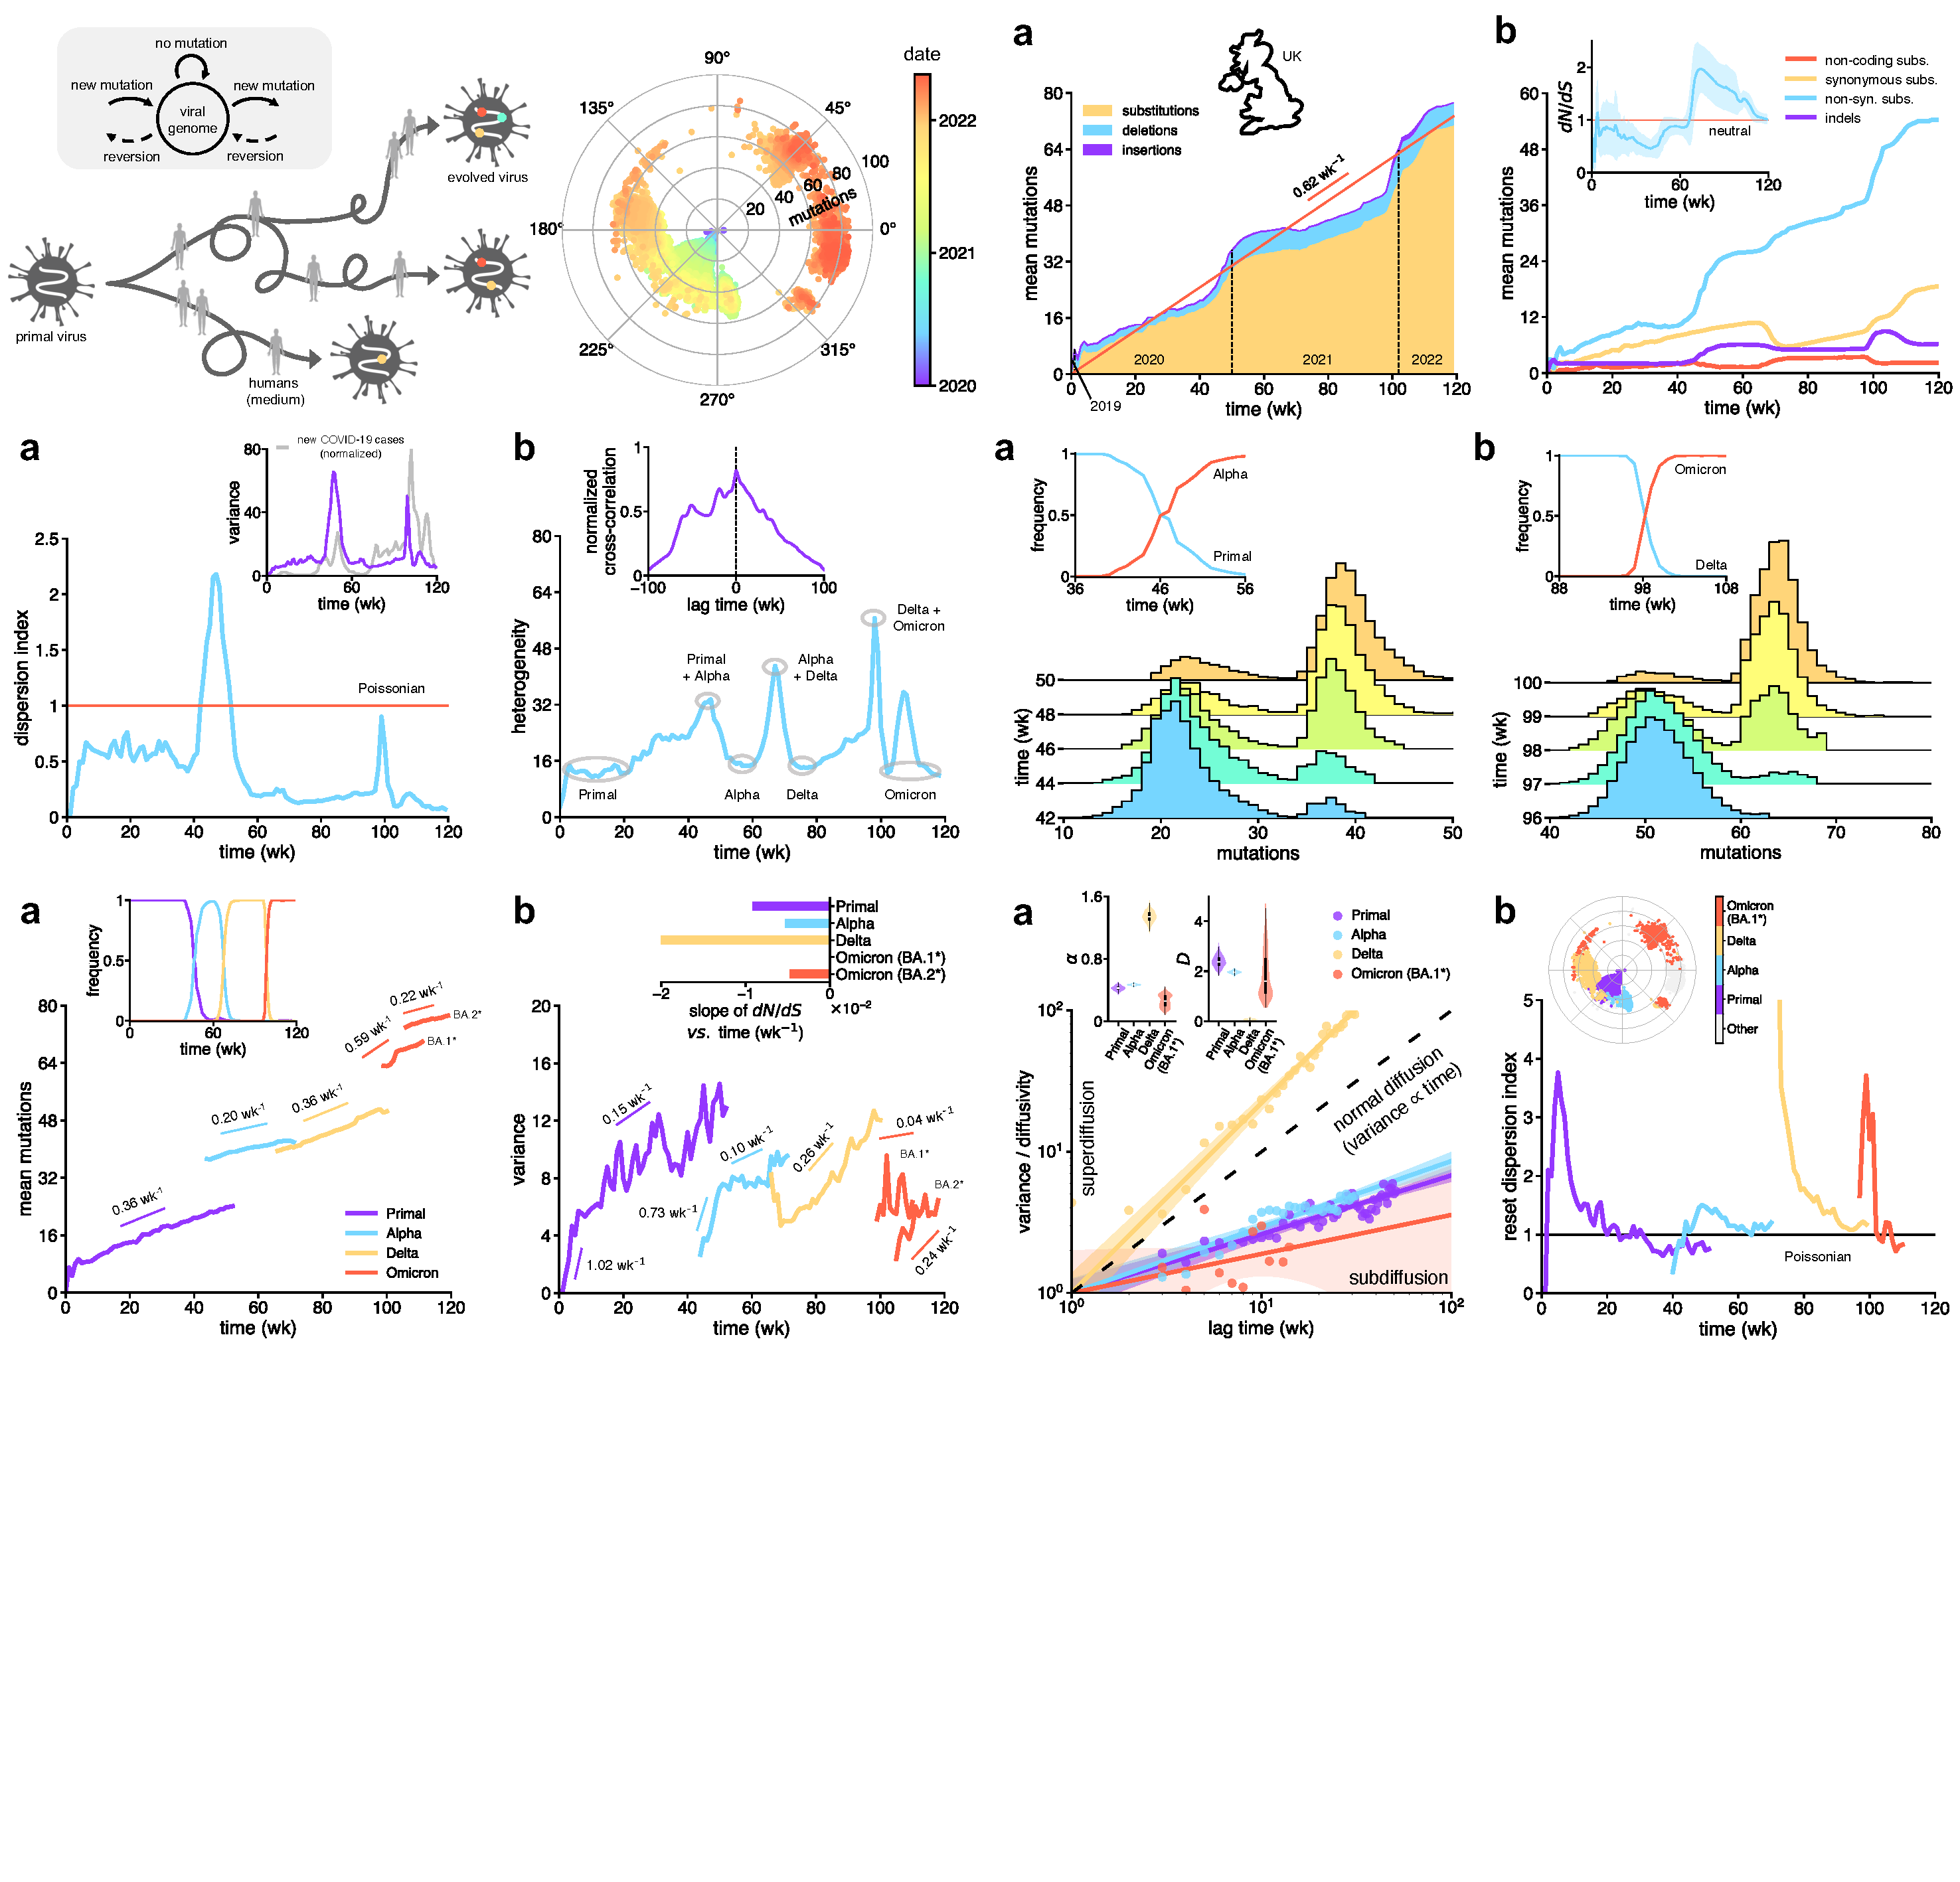
\includegraphics[trim={0 37.5cm 36.5cm 0.5cm},clip, width=0.67\linewidth]{assets/Ch2Fig.pdf}
    \caption{Schematics of the evolutionary motion of the virus (viewed as a stochastic process). Inset: associated state-transition diagram.}\label{fig:fig2.1}
\end{figure}
\vfill
\section{Results}\label{sec:results}

We sought to characterize the mean and variance (mean squared displacement) of the overall stochastic process by which the observable viral genome accumulates mutations with time (since the emergence in Wuhan, China). This was modeled in a continuous form by the Langevin equation:

\begin{equation}
    \frac{dm(t)}{dt}=\kappa + \xi(t)\label{eq:solution-model},
\end{equation}

\noindent where $m(t)$ is the total number of mutations in the genome at time $t$, $\kappa$ the evolution rate (which could be time-dependent), and $\xi(t)$ an integrative noise source whose properties shape the evolutionary motion.

Due to the large number of available SARS-CoV-2 sequences from United Kingdom (UK), our analysis was focused on this country. Using landmark multidimensional scaling (LMDS) \cite{deSilva2003}, we obtained a representation of all available genotypes in a two-dimensional space (\textbf{Fig. \ref{fig:fig2.2}}), which served to appreciate the virus evolution as a complex diffusion process. In this polar plot, the radius represented the number of mutations and the angle encompassed the rest of sequence variation.

\begin{figure}[ht!]
    \centering
    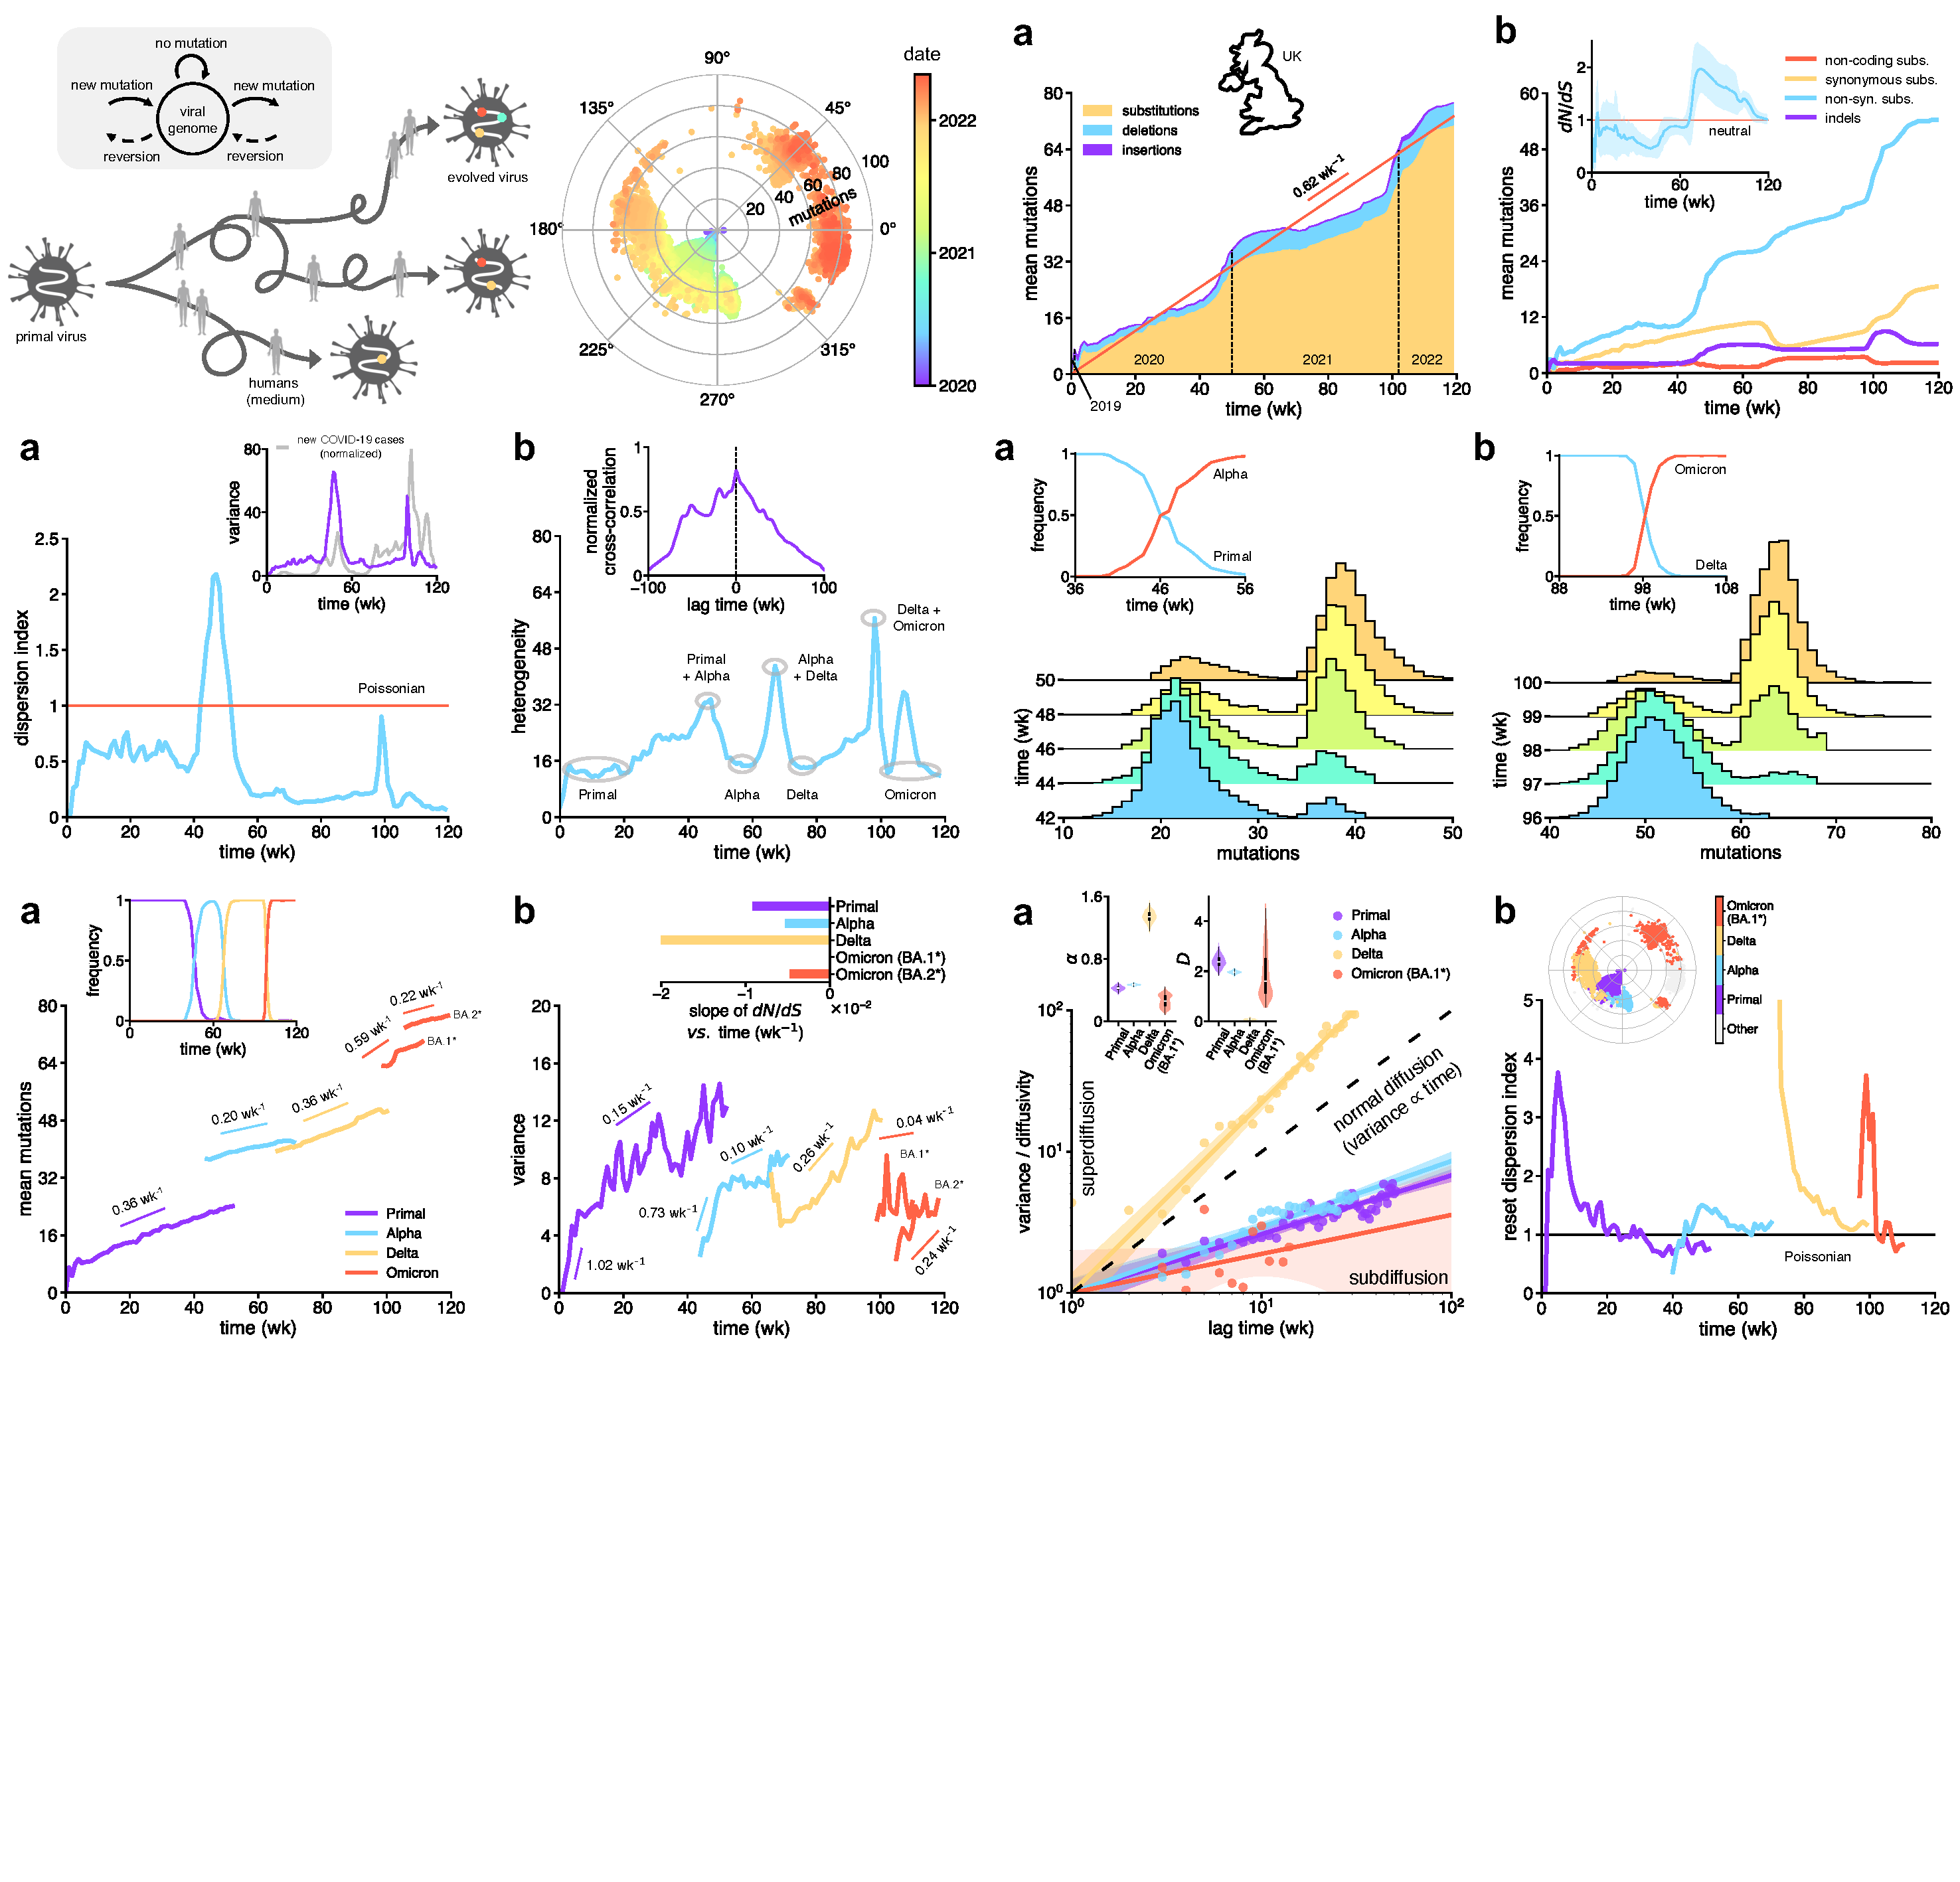
\includegraphics[trim={13.533cm 37.5cm 25.1cm 1cm},clip, width=0.5\linewidth]{assets/Ch2Fig.pdf}
    \caption{2D projection of all viral sequences colored by date.}\label{fig:fig2.2}
\end{figure}

To characterize the stochastic process, we first quantified the rate at which the viral genome accumulates a mean number of mutations with time. Considering all types of mutations and discretizing time by weeks (\textit{i.e.}, all sequences available in a week were pooled together), we obtained a macroscopic evolution rate of 0.62 wk\textsuperscript{-1} (Pearson's correlation with no intercept, $P < 10^{-4}$; \textbf{Fig. \ref{fig:fig2.3}a}). Substitutions were much more frequent than insertions and deletions (indels). However, at some points (at the end of 2020 and of 2021), an acceleration in the evolution rate was observed, thereby deviating from a molecular clock model with constant rate. Yet, without phylogenetic inference, this picture just reflected population changes and not strict evolutionary paths. In addition, mutations were classified according to their type (\textit{viz.}, non-coding, synonymous, non-synonymous, and indels), and the ratio between the number of nonsynonymous and synonymous substitutions per site (dN/dS) was estimated (\textbf{Fig. \ref{fig:fig2.3}b}), which is a common tool to assess the strength and mode of natural selection \cite{nielsen2005}. The observed dN/dS signature (fluctuation around 1 over time) suggested evolution under purifying selection of a series of adapted variants.

\begin{figure}[ht!]
    \centering
    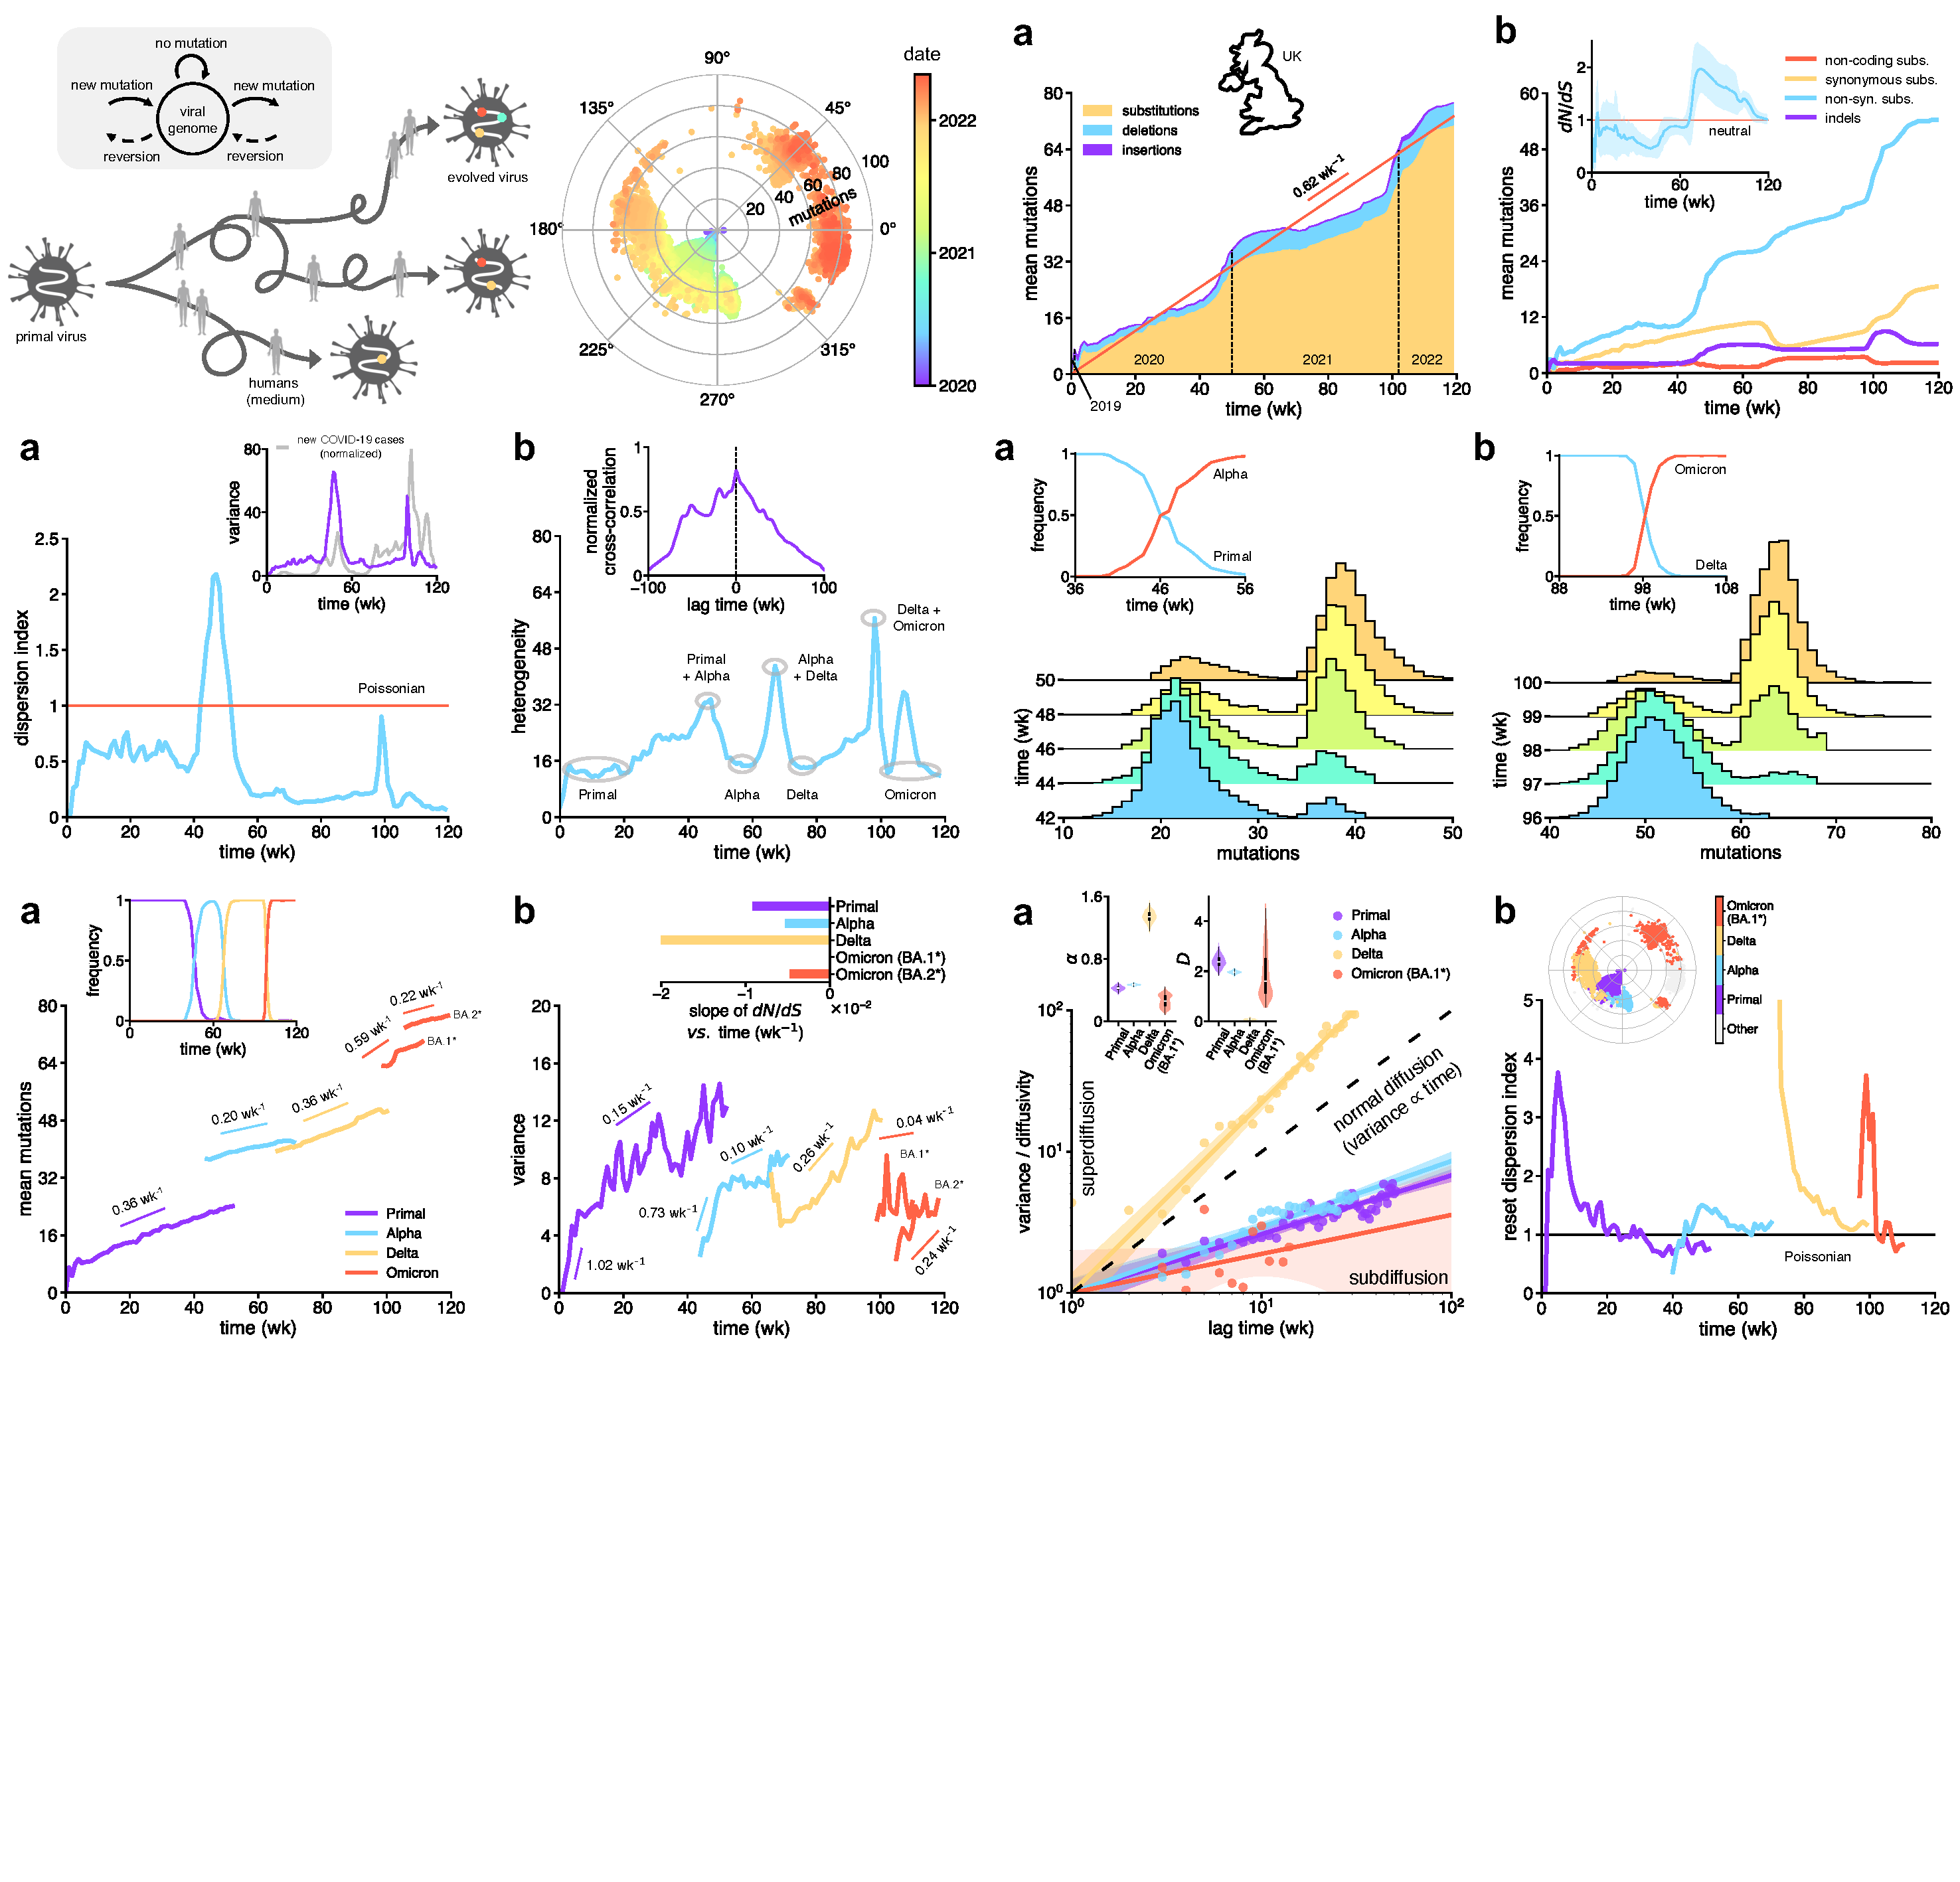
\includegraphics[trim={25.8cm 37cm 0 0.2cm},clip, width=\linewidth]{assets/Ch2Fig.pdf}
    \caption{a) Time-course of the mean number of accumulated mutations in the viral genome, distinguishing between substitutions, deletions, and insertions. Linear regression over the total shown in red (R\textsuperscript{2} = 0.95). b) Time-course of the mean number of non-coding substitutions, synonymous substitutions, non-synonymous substitutions, and indels. Inset: dN/dS with time (mean plus/minus standard deviation).}\label{fig:fig2.3}
\end{figure}

To test whether the accumulation of mutations in SARS-CoV-2 was a Poissonian stochastic process, we also calculated the variance and the dispersion index, understood as the ratio between variance and mean (\textbf{Fig. \ref{fig:fig2.4}a}). The study of the variance is often overlooked, despite it is essential to comprehend the evolutionary motion. We found largely sub-Poissonian dynamics (\textit{i.e}., dispersion index $<$ 1) with two main dispersion bursts at the times at which the evolution rate was accelerated. To inspect the origin of such a dynamic profile, we performed a sequence classification into variants. For simplicity, four variants were considered, \textit{viz.}, Primal, Alpha, Delta, and Omicron.

We realized that the first dispersion burst corresponded to the transition from Primal to Alpha, while the second to the transition from Delta to Omicron (\textbf{Fig. \ref{fig:fig2.4}b}). The number of new coronavirus disease 2019 (COVID-19) cases also correlated with the variance (inset of \textbf{Fig. \ref{fig:fig2.4}a}). Representing the distributions of accumulated mutations with time, we disclosed a bimodal behavior during such transitions (\textbf{Fig. \ref{fig:fig2.5}a, b}), explaining the increased dispersion. The invading genotypes carried about 15-20 more mutations on average. Moreover, the transition from Alpha to Delta only generated a slight dispersion signal because both variants carried a similar number of mutations. Arguably, outlier SARS-CoV-2 genotypes in the existing distribution at a time led to the emergence of new variants, and the observed accelerations in evolution rate came from the inherent stochasticity of the evolutionary motion followed by rapid, mostly deterministic invasion events once a particular genotype acquired a selective advantage, such as higher transmissibility \cite{kraemer2021}. 

\begin{figure}[t]
    \centering
    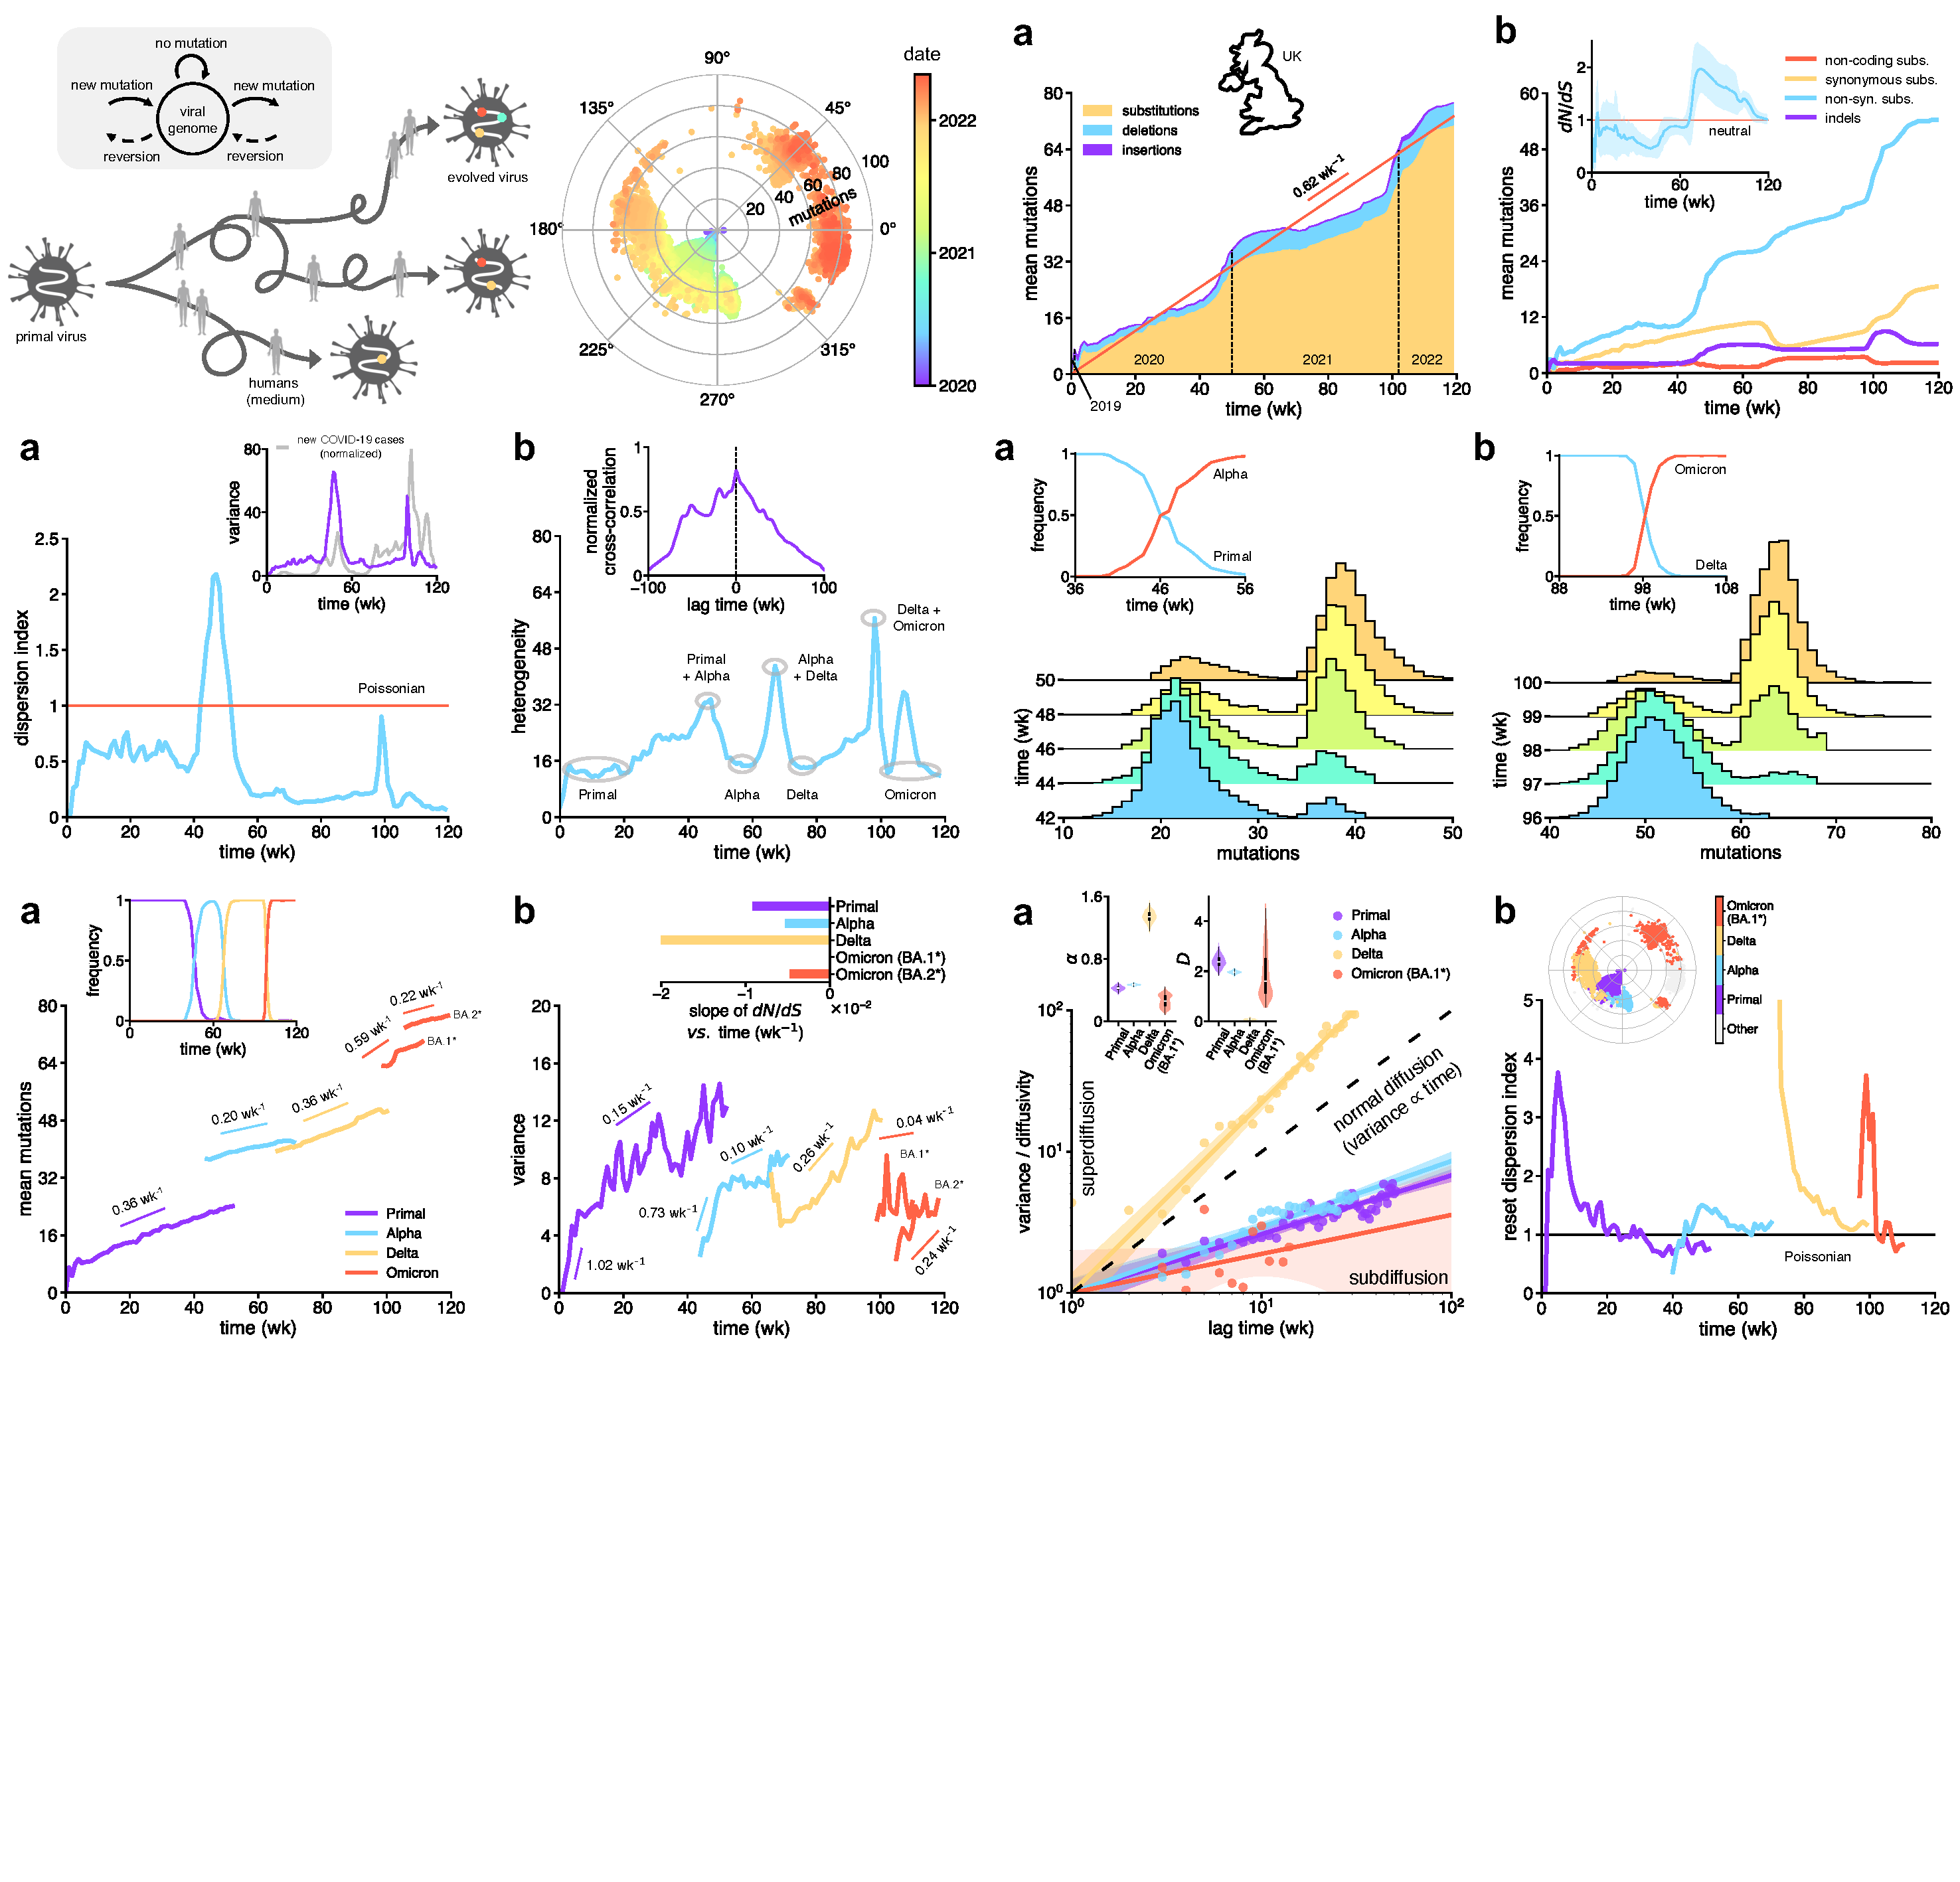
\includegraphics[trim={0.2cm 26cm 25.35cm 11cm},clip, width=\linewidth]{assets/Ch2Fig.pdf}
    \caption{a) Time-course of the dispersion index (variance/mean). Inset: variance with time; the normalized number of new COVID-19 cases is superimposed. b) Time-course of the degree of heterogeneity (mean Hamming distance), showing the different stages of the virus population in terms of variants. Inset: normalized cross-correlation between variance and heterogeneity with time.}\label{fig:fig2.4}
\end{figure}

Due to the virus population reset caused by the invasion of a new variant, we calculated the time-dependent statistics per variant. The analyses conducted for each variant were independent from each other by considering subsets of properly annotated sequences (\textit{i.e.}, no evolutionary paths between variants were considered). Of note, the evolution rates of Primal, Alpha, and Delta were substantially lower (up to 0.36 wk\textsuperscript{-1} ) than the inferred macroscopic value of 0.62 wk\textsuperscript{-1} (\textbf{Fig. \ref{fig:fig2.6}a}), in agreement with previous estimates following phylogenetic methods \cite{ghafari2022}. In the dataset, Omicron was composed of two lineages with sufficient dissimilarity, \textit{viz.}, BA.1 and BA.2 (BA.1 displaced Delta and BA.2 displaced BA.1). Performing a decomposition, we observed that BA.1 evolved faster than BA.2 in UK.\\

\begin{figure}[ht!]
    \centering
    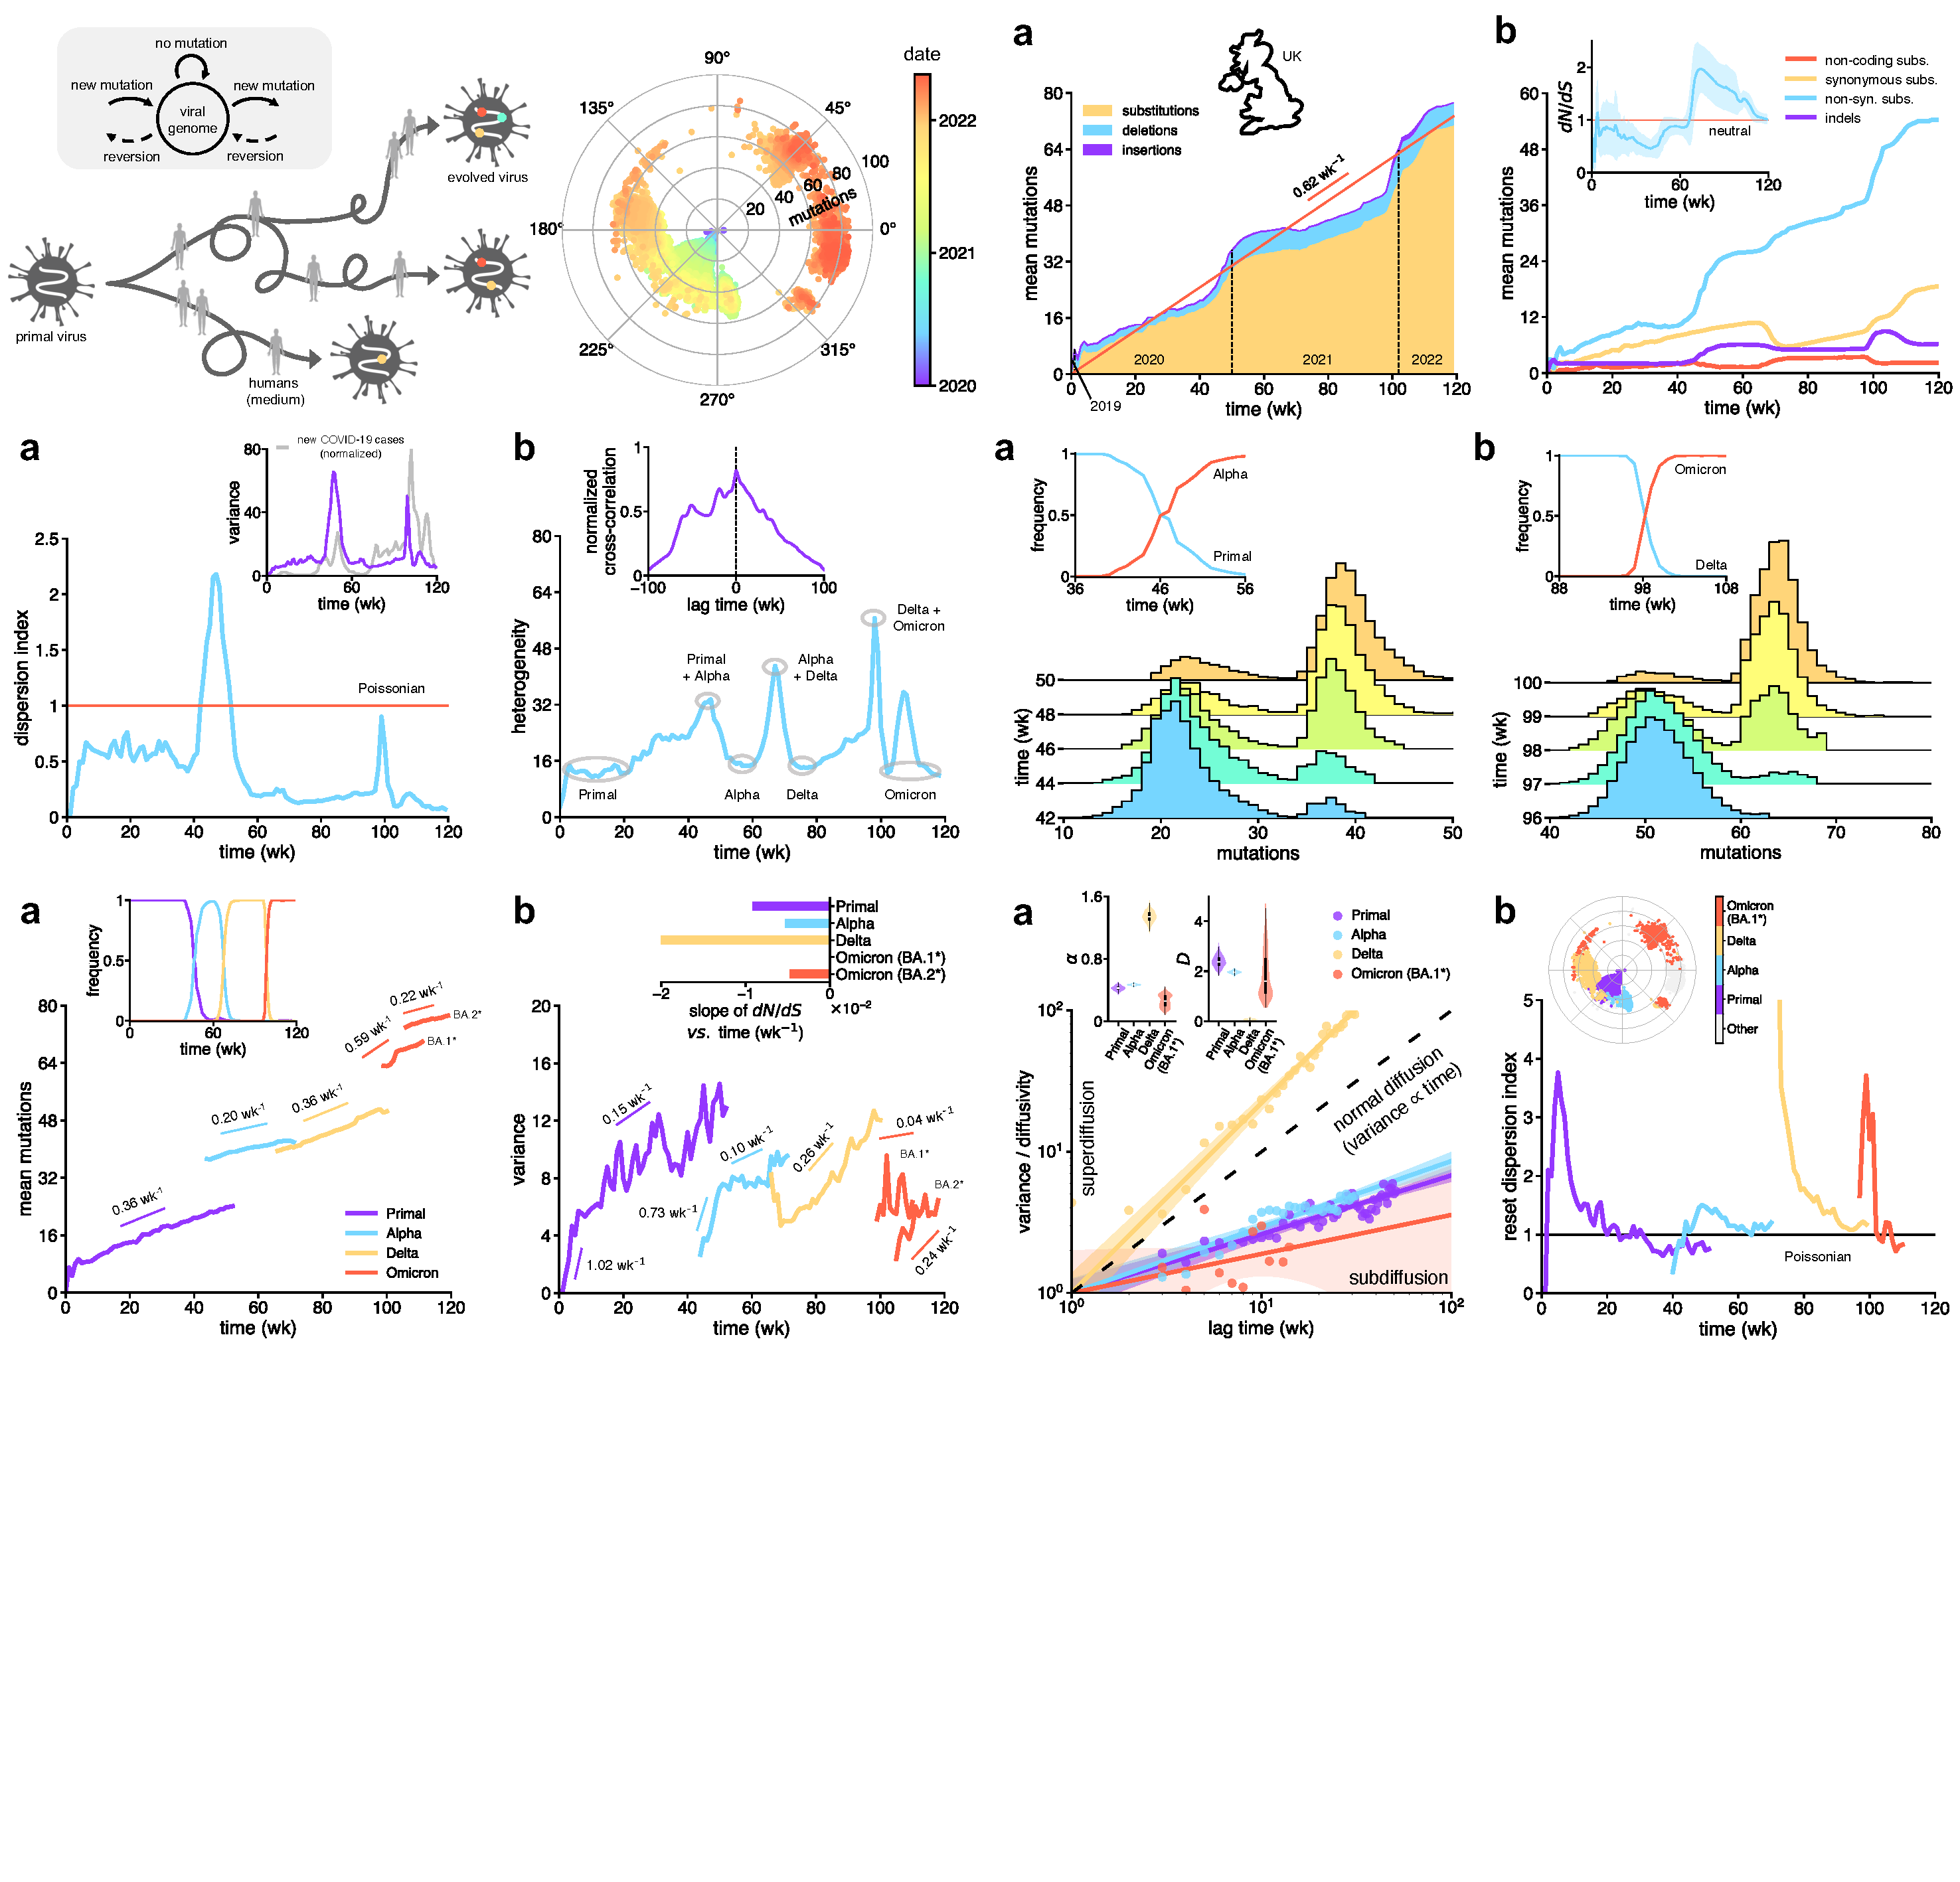
\includegraphics[trim={25.3cm 26cm 0.3cm 11cm},clip, width=\linewidth]{assets/Ch2Fig.pdf}
    \caption{Probability-based histograms of the number of accumulated mutations during the transition from Primal to Alpha (a) and Delta to Omicron (b). Insets: population frequency of the variants with time.}\label{fig:fig2.5}
\end{figure}

Collectively, the mean evolutionary motion was well captured by

\begin{equation}
    \mathbb{E}\left[m(t)\right] = \kappa t,
\end{equation}

\noindent with a constant variant-dependent rate, considering $\mathbb{E}\left[\xi (t)\right] = 0$ (Pearson's correlations, $P < 10^{-4}$ in all cases). In addition, we found significant nonlinear dependencies of the variance with time in all cases (Fisher-Snedecor's $F$ tests, $P < 10^{-4}$ for Primal, Alpha, and Delta, $P = 0.027$ for Omicron BA.1, and $P = 0.0003$ for Omicron BA.2; \textbf{Fig. \ref{fig:fig2.6}b}), which indicated a stochastic behavior with anomalous diffusion \cite{manzo2015}. In other words, SARS-CoV-2 underwent a non-Brownian evolutionary motion. This exciting result entailed that the explorations of the genotypic space by the virus to discover new phenotypes at different times were not fully uncorrelated within a clade.

To provide a quantitative picture of the process, we fitted $\mathbb{V}\left[m(t)\right]$ to the general expression $Dt^\alpha$, where $D$ is the diffusion coefficient and $\alpha$ the diffusion exponent. This expression is derived using the approaches shown in \textbf{Section \ref{sec:evolution-approximated-as-a-continuous-stochastic-process}} by considering 

\begin{equation}
    \text{Cov}\left[\xi(t),\xi(s)\right] = \frac{1}{2}D\alpha (\alpha - 1)\left|t - s\right|^{\alpha - 2}
\end{equation}

\noindent as the covariance function of the noise source $\xi(t)$. We found subdiffusion ($\alpha$ = 0.42, $\alpha$ = 0.47, and $\alpha$ = 0.28, respectively) in the cases of Primal, Alpha, and Omicron BA.1, while weak superdiffusion ($\alpha$ = 1.34) in the case of Delta (Pearson's correlations in log scale, $P < 10^{-4}$ for Primal, Alpha, and Delta and $P = 0.020$ for Omicron BA.1; \textbf{Fig. \ref{fig:fig2.7}a}). Although not plotted, we also found subdiffusion for Omicron BA.2 ($\alpha$ = 0.37). The robustness of these results was assessed by bootstrapping, \textit{i.e.}, performing a sampling with replacement of the sequences available each week in the original dataset and recomputing the dynamic profile of the variance. This also allowed dealing with the sequence pseudoreplication issue due to a shared history. Tolerable uncertainties for the diffusion parameters were noticed (inset of \textbf{Fig. \ref{fig:fig2.7}a}).

\begin{figure}[ht!]
    \centering
    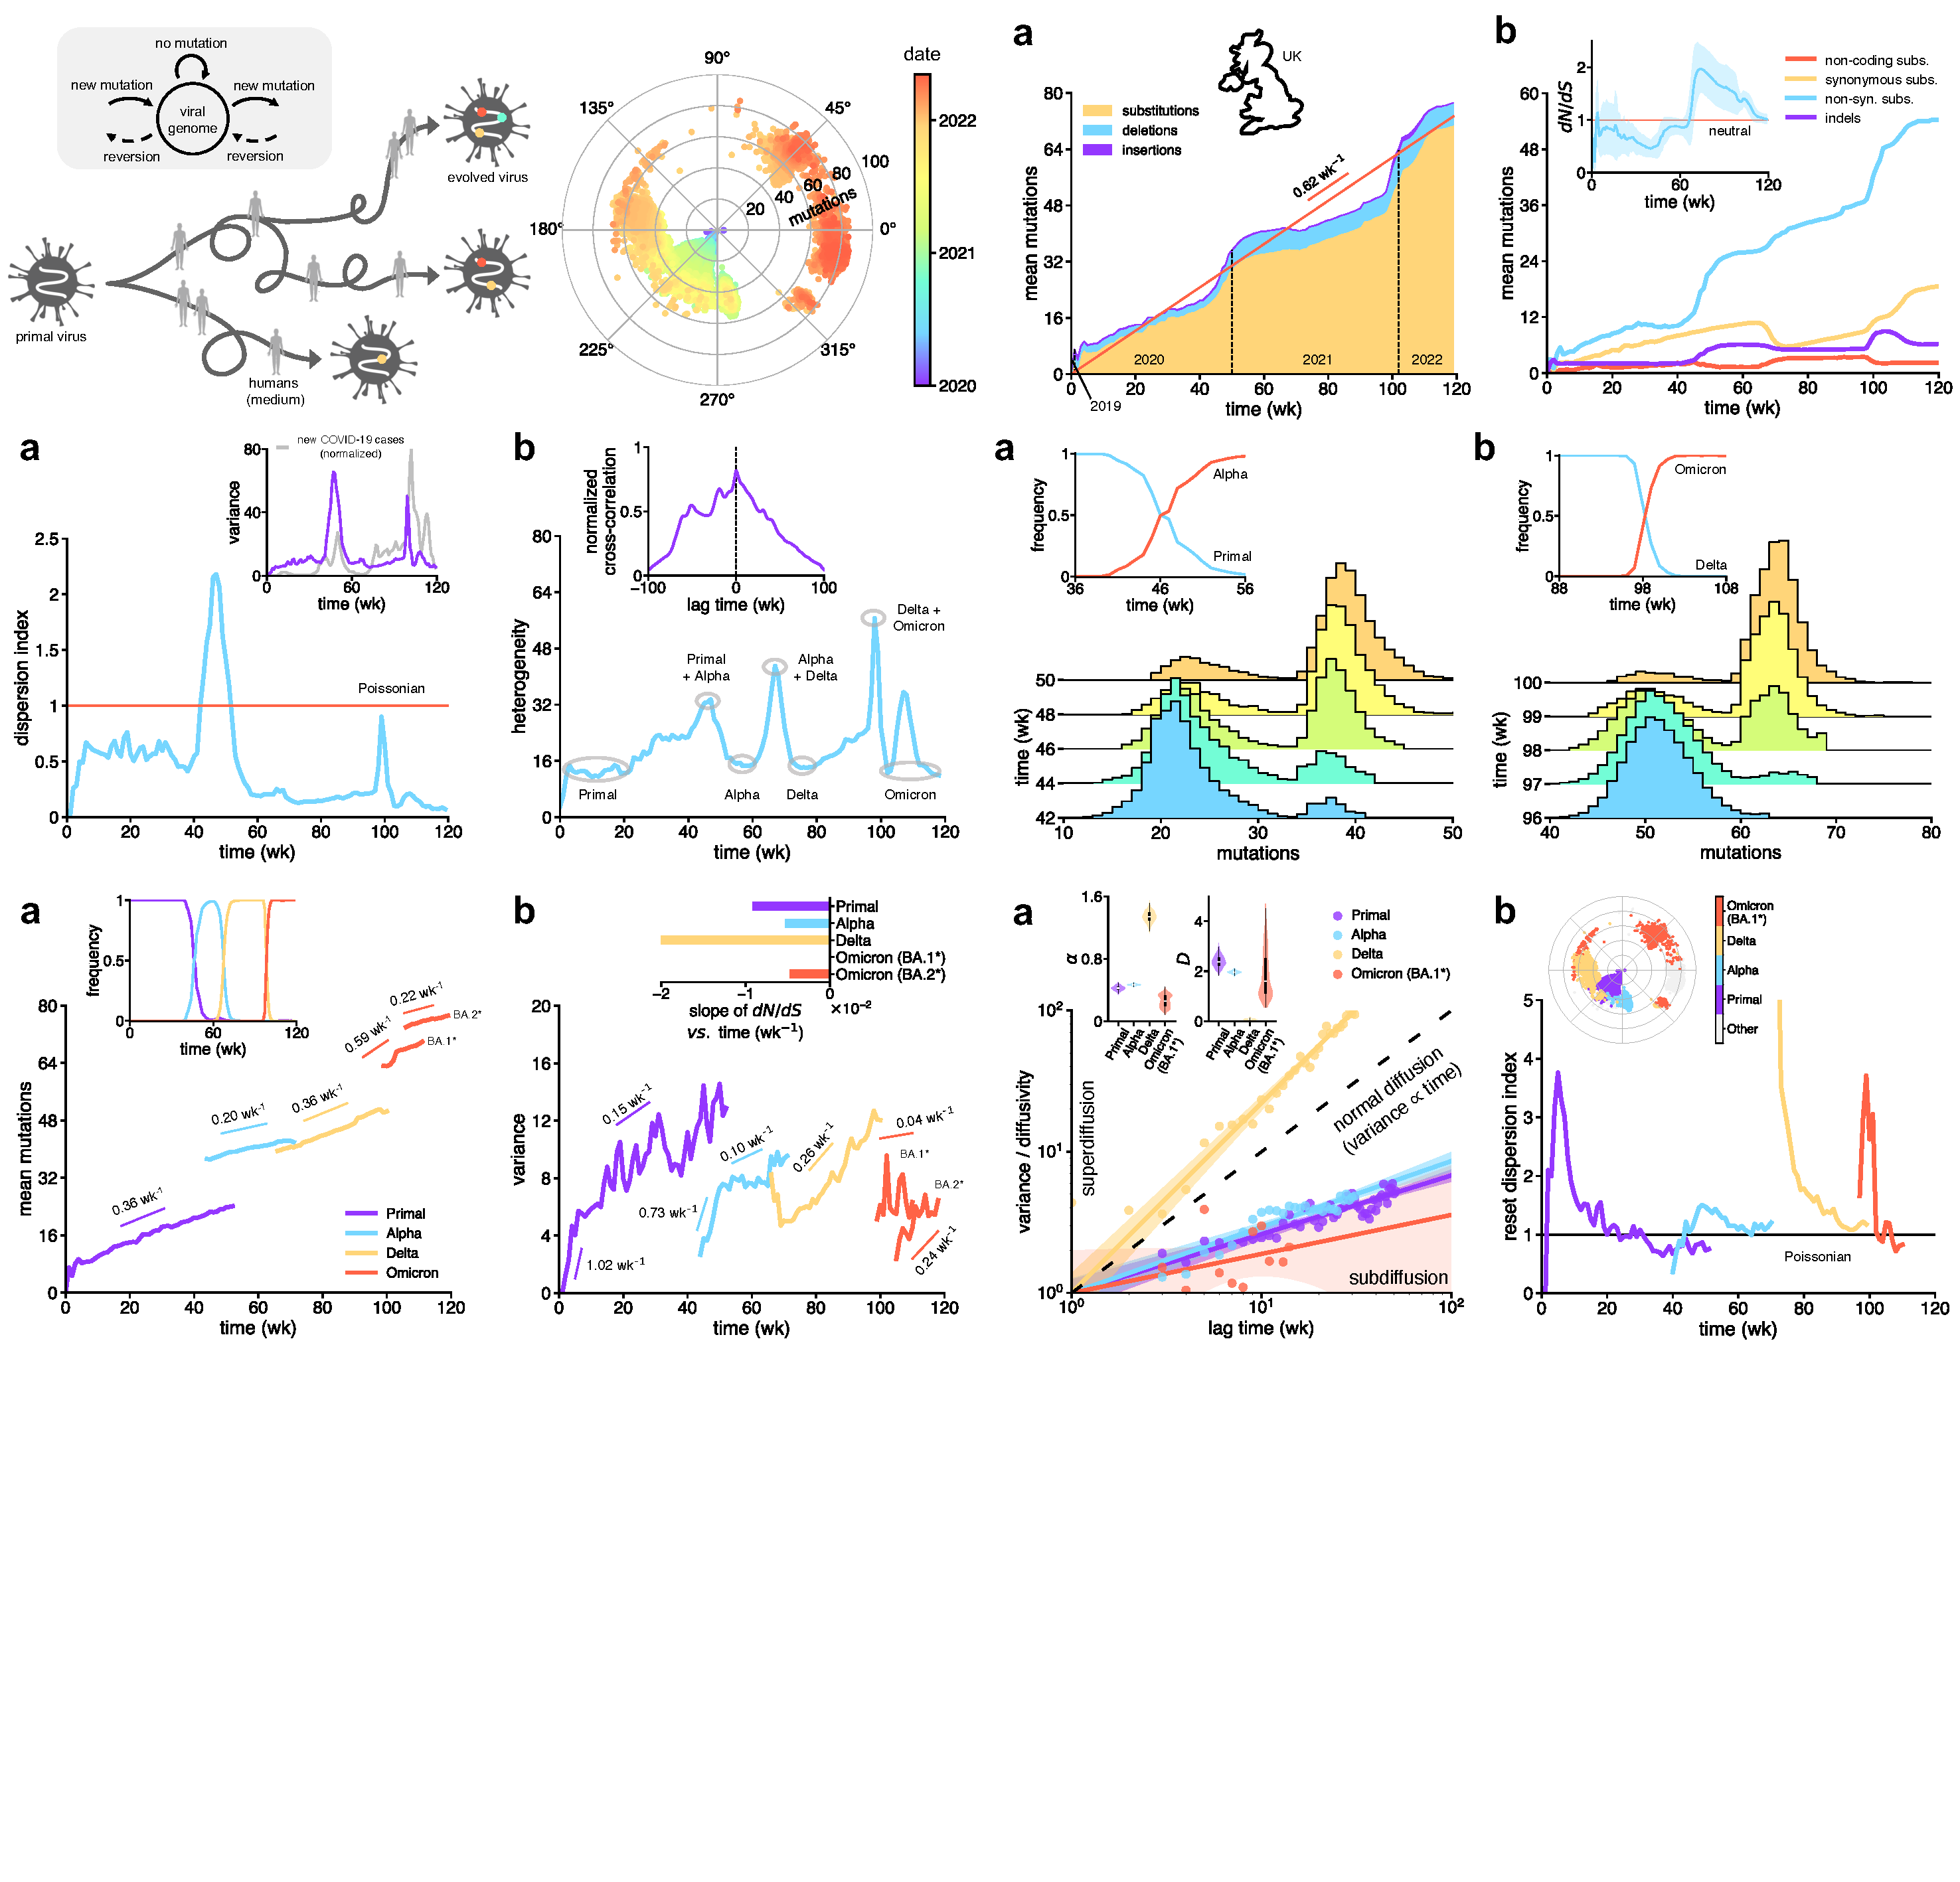
\includegraphics[trim={0.2cm 13.5cm 25.35cm 22.5cm},clip, width=\linewidth]{assets/Ch2Fig.pdf}
    \caption{a) Time-course of the mean number of accumulated mutations per variant (Omicron decomposed into BA.1 and BA.2). Linear regressions shown in each case (R\textsuperscript{2} $\geq$ 0.90). Inset: population frequency of the variants with time. b) Time-course of the variance per variant. Piecewise linear regressions shown in each case. Inset: slope of dN/dS with time for each variant obtained by linear regression.}\label{fig:fig2.6}
\end{figure}

To inspect the origin of anomalous diffusion in evolutionary motion, the rate at which the dN/dS ratio changed with time was analyzed per variant (inset of \textbf{Fig. \ref{fig:fig2.6}b}). We observed a decreasing trend in all cases, more pronounced for Delta. This suggested that Delta evolved by accumulating more synonymous mutations per site than the other variants. If these mutations were neutral \cite{deMaio2021}, the evolved genotypes of Primal, Alpha, and Omicron BA.1 would be more constrained as a result of their non-synonymous mutations, thereby explaining, at least in part, the observed subdiffusion patterns. Furthermore, we calculated a reset dispersion index, considering the accumulation of mutations since the appearance of the variant of study (\textit{i.e.}, each time a new variant invades the population, the number of mutations is reset). At long times, we found values in the neighborhood of 1, revealing an asymptotic Poissonian behavior following this metric (\textbf{Fig. \ref{fig:fig2.7}b}).

\begin{figure}[t]
    \centering
    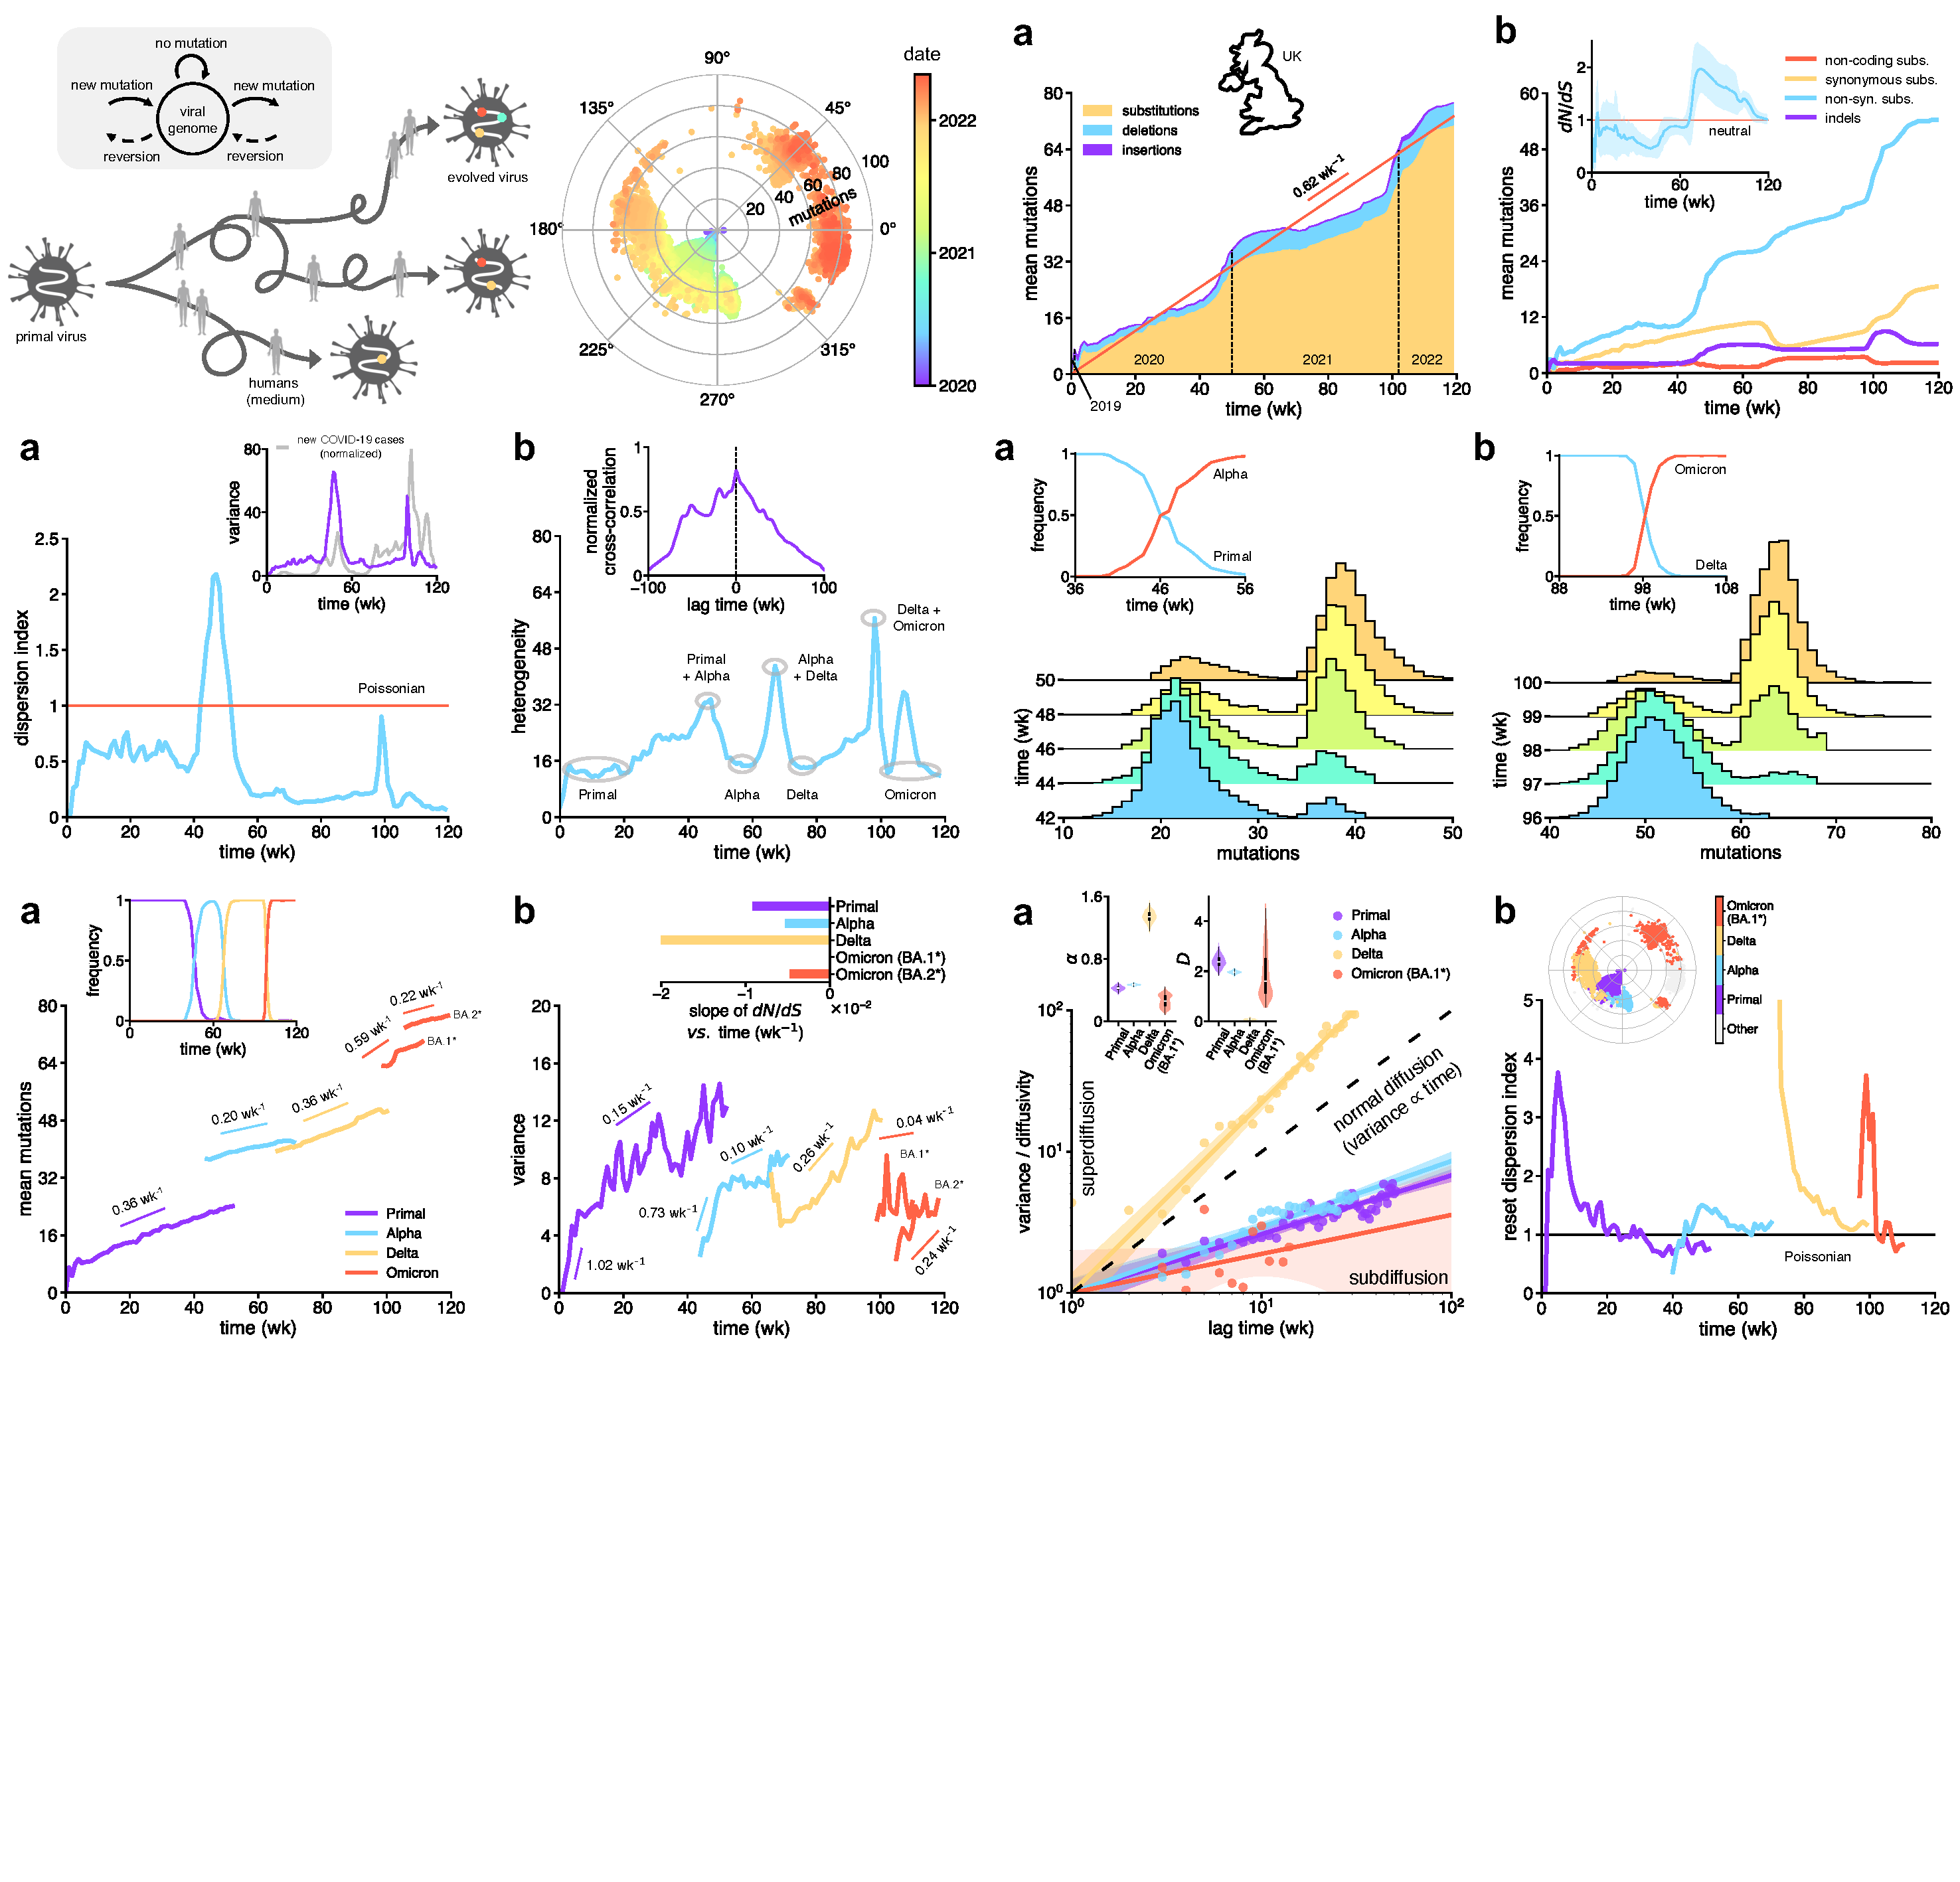
\includegraphics[trim={25.8cm 13.5cm 0.1cm 22.7cm},clip, width=\linewidth]{assets/Ch2Fig.pdf}
    \caption{a) Representation of the rescaled variance normalized by the diffusivity ($D$) with time in log scale (points correspond to data; for Primal, Alpha, Delta, and Omicron BA.1, R\textsuperscript{2} = 0.87, 0.88, 0.94, and 0.37, respectively, relative to Pearson's correlations in log scale). The slope of the fitted lines ($\alpha$) defines the type of diffusion ($\alpha>1$ superdiffusion, $\alpha<1$ subdiffusion). Shaded areas represent the 95\% confidence intervals of the regression lines. Inset: distributions of values for each diffusion parameter (violin plots) obtained by bootstrapping. b) Time-course of the reset dispersion index per variant. Inset: 2D projection of all viral sequences colored by variant (projection as in \textbf{Fig. \ref{fig:fig2.2}}). The variant-specific analyses were restricted to the time period in which their population frequency was at least 10\%.}\label{fig:fig2.7}
\end{figure}

\section{Discussion}

The observation of patterns of anomalous diffusion in biology has opened new avenues of research \cite{manzo2015}. Intriguingly, recent studies in which the physical movement of single SARS-CoV-2 virions was monitored throughout the infectious cycle highlighted transient and variant-dependent directionality and confinement outside and inside the cell \cite{christie2022, kreutzberger2022}, indicating deviation from a pure Brownian motion. Here, we have presented a new application domain in evolution. Of note, we uncovered that a probabilistic model with constant variant-dependent evolution rate and nonlinear mutational variance with time explained the SARS-CoV-2 evolutionary motion in humans during the first 120 weeks of pandemic in UK. This model might be used to refine phylodynamic approaches aimed at understanding the spread and adaptation of the virus. As shown, canonical descriptions based on the Poisson distribution do not accurately capture the observed dispersion at all time points.

These findings can also be situated within classical evolutionary theory, particularly Fisher's geometric model (FGM), which provides a quantitative framework to describe how organisms adapt in high-dimensional trait spaces.

\begin{definition}[Fisher's Geometric Model]
    Fisher's Geometric Model (FGM) conceptualizes the phenotype of an organism as a point $x \in \mathbb{R}^n$ in an $n$-dimensional Euclidean trait space, where each dimension represents an independent quantitative trait under stabilizing selection. The phenotypic optimum, corresponding to maximal fitness, is located at the origin of this space. The fitness of a phenotype $x$ is given by:
    
    \begin{equation}
        W(x) = W_0 \exp\left(-\frac{\|x\|^2}{2\sigma^2}\right),
    \end{equation}
    
    where $W_0 > 0$ denotes the maximal attainable fitness, $\sigma^2$ controls the strength of stabilizing selection (i.e., the curvature of the fitness landscape), and $\|x\|^2$ is the squared Euclidean distance from the phenotypic optimum. Mutational effects are modeled as random, isotropic displacements in phenotype space. The model predicts that the probability of a mutation being beneficial decreases as the phenotype approaches the optimum and increases with trait-space dimensionality $n$.
\end{definition}
    

Mutations correspond to random displacements $\Delta x$ in phenotype space, drawn from a symmetric distribution. The likelihood that a mutation increases fitness decreases with proximity to the optimum and increases with dimensionality $n$, due to the geometry of high-dimensional spaces. As a result, FGM predicts a declining rate of adaptation as populations approach a fitness peak \cite{couce2015}, along with a predominance of small-effect beneficial mutations. These properties make it a useful null model for interpreting adaptive dynamics in evolving populations \cite{tenaillon2014}.

In light of FGM, our findings offer both congruences and challenges. The subdiffusive mutational dynamics observed for Alpha and Omicron BA.1 variants are consistent with populations exploring a constrained phenotypic region near a fitness optimum, where evolutionary motion becomes increasingly restricted, an outcome that aligns with FGM's expectation of diminishing returns on adaptation. In contrast, the weak superdiffusive behavior seen in Delta reflects a more expansive phenotypic trajectory, possibly indicating that this variant originated from a population still far from the optimum and with greater adaptive potential. However, the punctuated emergence of variants with large mutational jumps, often involving dozens of substitutions, suggests evolutionary leaps not easily reconciled with FGM's assumption of small-effect mutations and a static fitness landscape \cite{miller2011}. These deviations may stem from shifts in host immunity, transmission dynamics, or selective pressures that effectively relocate the optimum over time. Furthermore, FGM's assumption of isotropic, additive mutational effects is likely violated in the context of SARS-CoV-2, where epistasis and context-dependent interactions are pervasive.

While FGM provides a valuable conceptual scaffold for interpreting our results within classical evolutionary theory, it falls short of fully capturing the complexity of SARS-CoV-2 dynamics. A more complete model would require generalizations that account for moving or rugged fitness landscapes, pervasive epistasis, and non-additive mutational effects, factors increasingly recognized as central to viral evolution. In parallel it is worth to note the bias in this type of studies caused by the fact that most of the sequenced viral genomes came from symptomatic infected people. Another issue is the imbalance in sequencing effort among countries, which prevents performing comprehensive analyses at a global scale. Further studies are required to assess the potential impact of movement and contact restrictions, vaccination, and self-diagnostic testing on the observed dynamic patterns. Overall, we anticipate deep implications of our data-driven results for future evolutionary and genomic studies, especially when dealing with fast evolving biological agents such as viruses.


\section{Materials and Methods}

\subsection{Whole-genome sequencing data}

The nucleotide sequences of the SARS-CoV-2 genomes used in this study were retrieved from the GISAID database (\url{https://www.gisaid.org}). As of May 2022, 10791877 sequences and the corresponding metadata were downloaded. Our analysis was restricted to the data from UK, which consists of 2735543 sequences. 

\subsection{Pairwise sequence alignments}

The nucleotide sequences of the SARS-CoV-2 genomes were aligned against a reference genome by means of Multiple Alignment using Fast Fourier Transform (MAFFT) \cite{katoh2002}. The results were collected in Clustal format. In this work, the reference sequence (root) was \texttt{hCoV-19/Wuhan/IVDC-HB-01/2019} (\texttt{EPI\_ISL\_402119}), which has 100\% identity with the GeneBank reference genome (\texttt{NC\_045512.2}) as shown by a Clustal Omega \cite{sievers2011} alignment.

\subsection{Construction of a functional dataset}

For each sequence, the number of mutations (substitutions, insertions, and deletions) with respect to the reference SARS-CoV-2 genome were counted. This information was retrieved from the MAFFT output alignments. In addition, the sequence collection dates and Pangolin lineages were retrieved from the metadata. Next, the sequences with unreliable recorded dates, whose unresolved base content surpassed 1\% (proportion of \texttt{N}s), or whose size was below 25 kb were discarded, as they were considered of low quality. Duplicated entries in the dataset were also removed. Furthermore, sequences isolated from non-human hosts were discarded. Then, the variant names were assigned where applicable based on the Pangolin lineage annotation. The Pangolin lineage-to-variant mapping was performed with information available at the Cov-lineages initiative (\url{https://cov-lineages.org}). All sequences dated earlier than 21 February 2021 were annotated as Primal variant (\textit{i.e.}, the original SARS-CoV-2 variant from Wuhan). The sequences were grouped by weeks. Finally, for each week, mutation outliers were filtered out to avoid artifacts in the calculated statistical parameters. These outliers could originate from incorrect date annotations, aberrant evolutionary trajectories, or sudden point introduction \cite{hill2022, michaelsen2022}. For each week, if the number of sequences was greater than 20, a Generalized Extreme Studentized Deviate (GESD) many-outlier procedure was applied \cite{rosner1983}. Otherwise, a filtering based on interquartile ranges was performed (\textit{i.e.}, the upper/lower bound was equal to the first/third quartile point plus/minus the interquartile range).

All data analyses were performed in Python using the libraries Pandas (\url{https://pandas.pydata.org}), NumPy (\url{https://numpy.org}), SciPy (\url{https://scipy.org}), Scikit-learn (\url{https://scikit-learn.org}), and Biopython (\url{https://biopython.org}).

\subsection{Landmark multidimensional scaling} %%% Ampliar?

Landmark multidimensional scaling (LMDS) is a variation of classical multidimensional scaling (MDS) \cite{mead1992} used to analyze and visualize dissimilarities between items based on a set of pairwise distance measures. The technique uses a small number of landmark items to compute their pairwise distances and estimate the distances between the remaining items, which are then mapped into a low-dimensional space using MDS \cite{deSilva2003}. LMDS presents several advantages over traditional MDS, including reduced computational complexity, scalability, and flexibility, making it an appropriate tool for analyzing large and complex datasets.

LMDS and principal component analysis (PCA) are both techniques used for dimensionality reduction, but they have some fundamental differences in their goals and methods. In contrast to LMDS, PCA is used to identify the underlying structure in a dataset by finding the principal components that explain the most variance in the data, capturing this way the most important patterns in the data \cite{jolliffe2016}. The interpretation of the coordinates in the projection space of both techniques is different as well, with PCA representing the patterns of variation and MDS representing the similarities and dissimilarities among the data points.

To obtain a representation of all available sequences in a two-dimensional (2D) space, a procedure based on landmark multidimensional scaling (LMDS) was followed \cite{deSilva2003}. For that, the Hamming distance between any two sequences was calculated (given by the number of mutations that separate each other). Metric axioms (minimality, symmetry, and triangle inequality) hold for the Hamming distance, so LMDS can be applied. The following sequences were used as landmarks:

\begin{table}[ht!]
    \centering
    \begin{tabular}{|l|l|}
        \hline
        \small\texttt{hCoV-19/England/CAMC-C42AEA/2020} & \small\texttt{hCoV-19/England/LSPA-2E824E8/2021}\\
        \small\texttt{hCoV-19/England/PHEC-YYBI3UW/2021} & \small\texttt{hCoV-19/Scotland/NORT-YBF4CD/2021}\\
        \small\texttt{hCoV-19/England/LSPA-3DC3179/2022} & \small\texttt{hCoV-19/England/ALDP-3A3CE1D/2022}\\
        \small\texttt{hCoV-19/England/ALDP-2E0DCFC/2021} & \small\texttt{hCoV-19/Wales/PHWC-PYDUBM/2021}\\
        \small\texttt{hCoV-19/England/QEUH-F8AA01/2021} & \small\texttt{hCoV-19/Scotland/QEUH-9AD0C0/2020}\\
        \hline
    \end{tabular}
    \caption{Sequence identifiers of landmarks employed during LMDS analysis.}
\end{table}

Polar coordinates were used to project the sequences in a 2D space. For the sake of interpretability, the radius was directly the total number of mutations from root and the angle was obtained from the coordinates generated by LMDS. It is worth noting that the position of two sequences in the projection plane will be determined by their similarity according to the Hamming distance. Consequently, if two sequences have the same number of mutations but these mutations are different, they will be located in different regions of the plane (i.e., their angles will be different and the radius will be the same).


\subsection{Calculation of statistical parameters}

For each set of SARS-CoV-2 sequences in a week, the mean and variance of the number of accumulated mutations (including substitutions and indels) were computed. For this computation, only the number of mutations was considered, not their type (\textit{i.e.}, different sequences with the same number of mutations counted the same). Then, the dispersion index was calculated, defined as the ratio between variance and mean. In addition, the mean Hamming distance between all sequence pairs in a week was computed to realize the extent of sequence heterogeneity. To compute the normalized cross-correlation between mutational variance and sequence heterogeneity, the \texttt{correlate} function from NumPy was used, having previously divided the statistical parameters by their norm (using the \texttt{linalg.norm} function). Finally, the number of COVID-19 cases in UK was retrieved from the database Our World in Data (\url{https://ourworldindata.org/}). The weekly number of new cases was computed. Probability-based histograms of the total number of mutations were obtained with the NumPy \texttt{histogram} function (\texttt{density=True}).

The calculation of mutational mean and variance was also performed per variant. This was done for the major lineages Primal, Alpha, Delta, and Omicron \cite{daCosta2022}, considering only the time period in which the variant represented at least the 10\% of the population. This limit was applied to avoid artifacts in the calculated statistical parameters due to a low number of sequences. In the case of Omicron, the calculation was performed for the sublineages BA.1 and BA.2 because of their great difference in mutations \cite{kumar2022}. For each variant, a reset dispersion index was also calculated, defined as the ratio between variance and the mean number of accumulated mutations since the first appearance of the variant in the population (\textit{i.e.}, each time a new variant invades the population, the number of mutations is reset). To some extent, this is in tune with the definition of a founder genotype for each clade from which to start counting as done in ref. \cite{neher2022}.

Specifically, if there are $N_k$ sequences in the $k$\textsuperscript{th} week, the mean number of accumulated mutations in that week, denoted by $\mathbb{E}\left[m_k\right]$, is calculated as follows:

\begin{equation}
    \mathbb{E}\left[m_k\right]=\frac{1}{N_k}\sum_{i=1}^{N_k}m_{k,i}\quad,
\end{equation}

\noindent where $m_{k,i}$ is the number of mutations of the $i$\textsuperscript{th} sequence in the $k$\textsuperscript{th} week. And the unbiased variance, denoted by $\mathbb{V}\left[m_k\right]$, is calculated as

\begin{equation}
    \mathbb{V}\left[m_k\right]=\frac{1}{N_k - 1}\sum_{i=1}^{N_k}\left(m_{k,i}-\mathbb{E}\left[m_k\right]\right)^2.
\end{equation}

To perform the calculations for a particular variant $v$, only the sequences annotated as such were considered (note that one sequence is linked at most to one particular variant). If there are $N_{v,k}$ sequences in the $k$\textsuperscript{th} week for variant $v$, the mean number of accumulated mutations in that week, denoted by $\mathbb{E}\left[m_{v,k}\right]$ is calculated as

\begin{equation}
    \mathbb{E}\left[m_{v,k}\right]=\frac{1}{N_{v,k}}\sum_{i=1}^{N_{v,k}}m_{v,k,i}\quad,
\end{equation}

\noindent where $m_{v,k,i}$ is the number of mutations of the $i$\textsuperscript{th} sequence in the $k$\textsuperscript{th} week annotated as variant $v$. And the variance, denoted by $\mathbb{V}\left[m_{v,k}\right]$, is calculated as

\begin{equation}
    \mathbb{V}\left[m_{v,k}\right] = \frac{1}{N_{v_k}-1}\sum_{i=1}^{N_{v,k}}\left(m_{v,k,i}-\mathbb{E}\left[m_{v,k}\right]\right)^2.
\end{equation}

Given that each sequence either belongs to a single variant, or to none, as a corollary of the above definitions the following relation holds:

\begin{equation}
    N_k=\sum_{v\in V}N_{v,k}+N_{\emptyset,k},
\end{equation}

\noindent where $V$ is the set of variants and $N_{\emptyset,k}$ denotes the number of sequences that are not linked to any variant of $V$ in the $k$\textsuperscript{th} week.

To assess the dispersion dynamics of the mutation distribution, the dispersion index ($\rho$) is used.

\begin{definition}[Dispersion Index]\label{def:dispersion_index}
    Given a stochastic process \( X(t) \) with finite mean \( \mathbb{E}\left[X(t)\right] \) and variance \( \mathbb{V}\left[X(t)\right] \), the Dispersion Index \( \rho(t) \), also known as the Fano Factor, is a measure of the relative variability of the process and is defined as

    $$
    \rho(t) = \frac{\mathbb{V}\left[X(t)\right]}{\mathbb{E}\left[X(t)\right]}
    $$
\end{definition}

\noindent Following \textbf{Definition \ref{def:dispersion_index}}, the dispersion index in the $k$\textsuperscript{th} week ($\rho_k$) is calculated as

\begin{equation}
    \rho_k=\frac{\mathbb{V}\left[m_{v,k}\right]}{\mathbb{E}\left[m_{v,k}\right]},
\end{equation}

\noindent and the reset dispersion index in the $k$\textsuperscript{th} week ($\rho_k^\text{reset}$) as

\begin{equation}
    \rho_k=\frac{\mathbb{V}\left[m_{v,k}\right]}{\mathbb{E}\left[m_{v,k}\right] - \mu_v},
\end{equation}

\noindent where $\mu_v$ is the mean number of mutations in the week in which $\mathbb{V}\left[m_{v,k}\right]$ is minimal. This condition corresponded to the first appearance of the variant of study in the population for Primal (first instance 26 Jan 2020), Alpha (first instance 25 Oct 2020), and Omicron BA.1 (first instance 21 Nov 2021), according to our functional dataset. In the case of Delta, however, the date of minimal variance did not coincide with the date of first instance, but rather with the moment at which the AY.4 lineage became dominant (16 May 2021) after a first period of time of selection within the Delta population, so this date was used for the mutation count reset.

\subsection{Global \textit{vs}. variant-based analysis}

The global analysis was carried out considering all available sequences from our functional dataset (\textit{i.e.}, pooling together the sequences even if they corresponded to different variants to compute the mean and variance for each week). This analysis served to appreciate the overall evolutionary trajectory by which the observable viral genome accumulates mutations with time in UK. That is, it allowed having a bird's eye perspective. More in detail, we could calculate a macroscopic evolution rate by linear regression between mean and time, and we could evaluate the dispersion dynamics of the resulting mutation distribution by representing the variance/mean ratio with time.

By contrast, the variant-based analysis was carried out considering only the sequences corresponding to a given variant, according to the annotation. This was done for Primal, Alpha, Delta, and Omicron (distinguishing also between the BA.1 and BA.2 lineages). Our analysis showed alternation of periods of evolution at lower rates and bursts of dispersion due to invasion events. We acknowledge that previous work already showed changes in the evolution rate with time in the particular case of SARS-CoV-2 \cite{ghafari2022, tay2022}. However, because our study was not based on phylogeny, we were able to process all available sequences in the database, gaining accuracy. In addition, and most importantly, because the dynamic profile of the variance was also analyzed, we were able to disclose anomalous diffusion patterns. This is a notable result that may contribute to change our understanding of virus evolution.

\subsection{Comparison with phylogenetic methods}

While in this work we are interested in how a viral population evolves, phylogenetic approaches mainly focus on genotypic differences in order to reconstruct evolutionary paths. Phylogenetic methods have been applied to produce estimates of the SARS-CoV-2 evolution rate, reporting values of 0.3-0.4 wk\textsuperscript{-1} during the first year of pandemic \cite{ghafari2022, wang2022}. These values are in tune with our calculations in the case of Primal. This congruence suggested us the formation with time of a sufficiently heterogenous viral population. Indeed, using the metric of heterogeneity, once a variant was fixed, the divergence between two arbitrary sequences of the population was about 11-15 mutations.

Further phylogenetic inferences have pointed out a transient increase of the evolution rate concomitant with the emergence of new invading variants (e.g., Alpha) \cite{tay2022}. However, by restricting the study to the sequences within the clade, the evolution rate did not appear to increase but rather to be maintained or even reduced (e.g., in the cases of Alpha and Delta). According to our analysis and also others in the field following non-phylogenetic approaches \cite{neher2022}, Alpha evolved a bit slower than Primal and Delta did at a similar rate. Despite the uncertainty associated with the emergence of new variants \cite{hill2022}, viral population- based studies are useful to understand the mutation-selection dynamics.

\subsection{Categorization of mutations}

For each viral sequence present in the functional dataset, the set of substitutions with respect to root were broken down into several categories: non-coding substitutions (\textit{i.e.}, substitutions that fall on non-coding regions of the genome), synonymous substitutions (\textit{i.e.}, substitutions that fall on coding regions but do not trigger amino acid changes), and non-synonymous substitutions (\textit{i.e.}, substitutions that trigger amino acid changes in coding regions). Insertions and deletions were counted into a unique variable called indels. Finally, the weekly mean and variance in terms of number of non-coding substitutions, synonymous substitutions, non-synonymous substitutions, and indels were computed.

\subsection{Estimation of natural selection signatures}

The ratio between the number of nonsynonymous and synonimous substitutions per site (dN/dS) was used to realize the sense of natural selection \cite{nielsen2005} during SARS-CoV-2 evolution, as it is a suitable statistical parameter to estimate the balance between positive (adaptive), neutral, and negative (purifying) selection acting on a set of protein-coding genes \cite{kryazhimskiy2008}. A simple method was employed to estimate the dN/dS ratio for each viral sequence \cite{nei1986}, assuming that:

\begin{enumerate}[i]
    \item The total length of the protein-coding genes was constant (equal to that of the reference genome).
    \item The four nucleotides had equal frequencies.
    \item The substitution events were random.
\end{enumerate}

First, the total number of synonymous ($S$) and non-synonymous ($N$) sites was estimated. Given that the probability of maintaining the same amino acid sequence is 5\% if the substitution occurs at the first position of the codon, 0\% if it occurs at the second position, and 72\% if it occurs at the third position, it turns out that $S\approx (0.05+0.72)R$  and $N\approx 3(R-S)$, where $R$ is the total length in base pairs of the protein-coding genes. Then, the proportion of synonymous ($p_S$) and non-synonymous ($p_N$) substitutions per site were computed. Second, these proportions were corrected to account for multiple potential changes at the same site. The genetic distance of synonymous ($d_S$) and non-synonymous ($d_N$) substitutions per site was estimated using the Jukes-Cantor formula. 

\begin{definition}[Jukes-Cantor Formula]
    Assuming equal base frequencies and equal probability of substition occurrence between any pair of nucleotides, the genetic distance can be approximated by

    $$
    d = -\frac{3}{4} \ln{\left(1 - \frac{4}{3}p\right)}
    $$

    where \(d\) is the estimated number of substitutions per site, and \(p\) is the observed proportion of nucleotide sites at which the two sequences differ \cite{jukes1969}.

    For the particular cases of synonymous (\(d_S\)) and non-synonymous (\(d_N\)) substitutions, the expression becomes

    $$
    \begin{cases}
        d_S = -\frac{3}{4} \ln{\left(1 - \frac{4}{3}p_S\right)}\\
        d_N = -\frac{3}{4} \ln{\left(1 - \frac{4}{3}p_N\right)}
    \end{cases}
    $$

    where \(p_S\) and \(p_N\) are the observed proportions of synonymous and non-synonymous nucleotide differences, respectively.
\end{definition}



\subsection{Mathematical modeling of evolutionary motion}

To motivate the development of a novel molecular clock model, we will briefly explore how a Poisson point process can be employed to model DNA sequence evolution. We then extend the Poisson point process into a continuous stochastic process, and finally present a model that captures the anomalous diffusion patterns observed in the evolutionary motion of SARS-CoV-2.

\subsubsection{Evolution as a Poisson point process}

The Poisson distribution is commonly used to model the occurrence of infrequent events within a fixed time or space interval. In the context of genetic mutations during DNA replication, each generation (defined as a replicative cycle) can introduce changes or substitutions in the DNA sequence due to various factors like errors induced by the DNA polymerase, radiation, or the presence of chemicals. Since the likelihood of a mutation at a specific position in the DNA sequence is assumed to be small, constant, and independent between generations (as supported by experimental evidence), the number of mutations in a lineage over $n$ generations can be accurately described using the Poisson distribution.



Let $u$ be the rate of mutations per generation, and $n$ the number of generations. In this scenario, the number of mutations that occur in a lineage during these $n$ generations follows a Poisson distribution with a mean value of $un$. In addition, if each generation takes the same amount of time, the number of mutations in the lineage during a specific time period $t$ can be described as a homogeneous Poisson point process, denoted as $\left\{N(t), t \geq 0\right\}$, where $N(t)$ represents the total number of mutations that have taken place up to (and including) time $t$. Consequently, the probability of observing exactly $n$ mutations, denoted as $N(t) = n$ at time $t$, is given by

\begin{equation}
    \text{Pr}(N(t) = n) = \frac{e^{-\kappa t}\left(\kappa t\right)^n}{n!}\label{eq:poisson},
\end{equation}

\noindent where $\kappa$ the rate of substitutions for a given unit of time. Importantly, \textbf{Equation \ref{eq:poisson}} implies that the number of mutations in a lineage at time $t = 0$ is $0$ and that the increments of the process are independent.

For further developments, it is convenient to compute the moment generating function, $M_{N(t)}(s)$, of the Poisson process:

\begin{align}
    M_{N(t)}(s) &= \mathbb{E}\left[e^{sN(t)}\right]\\
    &= \sum_{n=0}^{\infty} e^{sn} \frac{e^{-\kappa t}\left(\kappa t\right)^n}{n!}\nonumber\\
    &= e^{-\kappa t} \sum_{n=0}^{\infty} \frac{\left(\kappa t e^s\right)^n}{n!}\nonumber\\
    &= e^{-\kappa t} e^{\kappa t e^s}\nonumber\\
    &= e^{\kappa t (e^s - 1)}\label{eq:mgf}
\end{align}

By means of \textbf{Equation \ref{eq:mgf}} it is straightforward to demonstrate that the mean and variance of the process are both given by $\kappa t$:

\begin{align}
    \mathbb{E}\left[N(t)\right] &= \left.\frac{\partial}{\partial s}M_{N(t)}(s)\right|_{s=0}\\
    &= \left[\kappa t e^{\kappa t\left(e^s-1\right) + s}\right]_{s=0}\nonumber\\
    &= \kappa t\\
    \mathbb{V}\left[N(t)\right] &= \mathbb{E}\left[\left(N(t) - \mathbb{E}\left[N(t)\right]\right)^2\right]\\
    &= \mathbb{E}\left[N^2(t) -2N(t)\mathbb{E}\left[N(t)\right] + \mathbb{E}\left[N(t)\right]^2\right]\nonumber\\
    &= \mathbb{E}\left[N^2(t)\right] -\mathbb{E}\left[N(t)\right]^2\nonumber\\
    &= \left.\frac{\partial^2}{\partial s^2}M_{N(t)}(s)\right|_{s=0} - \left(\kappa t\right)^2\nonumber\\
    &= \left[\kappa t \left(\kappa t e^s + 1\right)e^{\kappa t\left(e^s - 1\right) + s}\right]_{s=0} - \left(\kappa t\right)^2\nonumber\\
    &= \left(\kappa t\right)^2 + \kappa t - \left(\kappa t\right)^2\nonumber\\
    &= \kappa t
\end{align}

As a corollary, and recalling \textbf{Definition \ref{def:dispersion_index}}, it is possible to assess that the process' dispersion index $\rho_{N(t)}$ is equal to $1$.

\subsubsection{Evolution approximated as a continuous stochastic process}\label{sec:evolution-approximated-as-a-continuous-stochastic-process}

Similar to how the Poisson distribution can be approximated by a Gaussian distribution through the central limit theorem, a Poisson point process can be approximated by a Wiener process. The Wiener process, also known as Brownian motion, is a continuous-time stochastic process characterized by independent and stationary increments. It is usually represented as $\left\{W(t), t \geq 0\right\}$, where $W(t)$ is a random variable representing the displacement of a particle at time $t$, its increments follow a normal distribution with a mean $\mathbb{E}[W(t)] = 0$ and, if it's the standard Wiener process, a covariance function $\text{Cov}[W(t), W(s)] = \min\left(t,s\right)$. The Wiener process is widely used as a model for random fluctuations in various physical systems.

Therefore, the number of mutations during DNA replication can be thought of a kind of \textit{random motion}, which we call \textit{evolutionary motion}, in the abstract space of all possible DNA sequences and it is defined as the following Langevin stochastic differential equation

\begin{equation}
    \frac{dm(t)}{dt} = \kappa + \sqrt{\kappa}\zeta(t)\label{eq:langevin},
\end{equation}

\noindent where $\zeta(t)$ is a Gaussian white noise characterized by $\mathbb{E}\left[\zeta(t)\right]=0$ and covariance function $\text{Cov}\left[\zeta(t),\zeta(s)\right]=\delta (t - s)$. Note that $\zeta(t)$ is defined as the formal derivative of the standard Wiener process $W(t)$, an assertion which has to be handled with caution because the Wiener process is nowhere differentiable with probability 1, therefore the Langevin formalism needs to be interpreted in a distributional sense. \textbf{Equation \ref{eq:langevin}} can be solved analytically:

\begin{align}
    \frac{dm(t)}{dt} &= \kappa + \sqrt{\kappa}\zeta(t)\nonumber\\
    m(t) &= m(0) + \kappa t + \sqrt{\kappa}\int_0^t \zeta(s)ds\label{eq:langevin-solution-dna}
\end{align}

\textbf{Equation \ref{eq:langevin-solution-dna}} can be further simplified given the number of mutations at time $t = 0$ is $0$:

\begin{align}
    m(t) &= m(0) + \kappa t + \sqrt{\kappa}\int_0^t \zeta(s)ds\nonumber\\
    &= \kappa t + \sqrt{\kappa}\int_0^t \zeta(s)ds\label{eq:langevin-solution-dna-simplified}
\end{align}

Note that the reformulation given at \textbf{Equation \ref{eq:langevin}}, which results in the solution at \textbf{Equation \ref{eq:langevin-solution-dna-simplified}}, maintains the original Poisson process' mean and variance:

\begin{align}
    \mathbb{E}\left[m(t)\right] &= \mathbb{E}\left[\kappa t + \sqrt{\kappa}\int_0^t \zeta(s)ds\right]\\
    &= \kappa t + \sqrt{\kappa}\mathbb{E}\left[\int_0^t\zeta(s)ds\right]\label{eq:langevin-mean-step1}\\
    &= \kappa t + \sqrt{\kappa}\int_0^t\mathbb{E}\left[\zeta(s)\right]ds\label{eq:langevin-mean-step2}\\
    &= \kappa t\label{eq:langevin-mean}
\end{align}

\begin{align}
    \mathbb{V}\left[m(t)\right] &= \mathbb{E}\left[\left(m(t) - \mathbb{E}\left[m(t)\right]\right)^2\right]\\
    &= \mathbb{E}\left[\left(\kappa t + \sqrt{\kappa}\int_0^t \zeta(s)ds - \kappa t \right)^2\right]\nonumber\\
    &= \kappa\mathbb{E}\left[\left(\int_0^t \zeta(s)ds\right)\left(\int_0^t \zeta(u)du\right)\right]\label{eq:langevin-variance-substep-a}\\
    &= \kappa\mathbb{E}\left[\int_0^t\int_0^t \zeta(s)\zeta(u)dsdu\right]\label{eq:langevin-variance-substep-b}\\
    &= \kappa\int_0^t\int_0^t \mathbb{E}\left[\zeta(s)\zeta(u)\right]dsdu\label{eq:langevin-variance-substep-c}\\
    &= \kappa\int_0^t\int_0^t \text{Cov}\left[\zeta(s),\zeta(u)\right]dsdu\label{eq:langevin-variance-substep-d}\\
    &= \kappa\int_0^t\int_0^t \delta(s-u) dsdu\label{eq:langevin-variance-substep-e}\\
    &= \kappa\int_0^t1du\nonumber\\
    &= \kappa t\label{eq:langevin-variance}
\end{align}

Note that the steps that involve \textbf{Equations \ref{eq:langevin-mean-step1}, \ref{eq:langevin-mean-step2}, \ref{eq:langevin-variance-substep-a}, \ref{eq:langevin-variance-substep-b}} and \textbf{\ref{eq:langevin-variance-substep-c}} are consequence of Fubini's theorem, which allows the interchange of the order of integration, as the integrals are known to be absolutely convergent and the fact that the expectation is a linear operator. The step that involves \textbf{Equations \ref{eq:langevin-variance-substep-c}} and \textbf{\ref{eq:langevin-variance-substep-d}} are consequence of the definition of covariance. The step that involves \textbf{Equations \ref{eq:langevin-variance-substep-d}} and \textbf{\ref{eq:langevin-variance-substep-e}} is a consequence of the definition of the Dirac delta functional. \textit{While the same result can be obtained through Itô's formalism, we will continue using Langevin's formalism due to its particular relevance in Biology.}

As a corollary, the corresponding dispersion index $\rho_{m(t)}$ remains equal to $1$ as expected, since the Wiener process is a continuous-time approximation of the Poisson process. One concern that arises from this reformulation is that the number of mutations $m(t)$ is no longer an integer, hence the model may not seem suitable for counting mutations in a lineage during a specific time period $t$. However, this issue can be easily solved by applying a rounding function to $m(t)$ whenever it is necessary to obtain an integer value.

\subsubsection{Anomalous Diffusion}

In the preceding section we demonstrated that, according to the molecular clock hypothesis, the number of mutations occurring in a lineage during a specific time period $t$ can be described as a Brownian motion (\textbf{Equation \ref{eq:langevin-solution-dna-simplified}}) exhibiting a mean and variance equal to $\kappa t$ (\textbf{Equations \ref{eq:langevin-mean}} and \textbf{\ref{eq:langevin-variance}}), where $\kappa$ represents the rate of substitutions for a given unit of time, akin to a microscopic particle moving in a fluid as a consequence of thermal forces.

However, it is well known that the diffusion of microscopic particles in a fluid does not always conform to Brownian motion. In fact, the diffusion of particles in a fluid can be classified into three main categories depending on their mean squared displacement (MSD; also understood as the variance of the stochastic process governing the motion): normal diffusion, subdiffusion, and superdiffusion. Under normal diffusion, the MSD of the particle is proportional to $t$, while under subdiffusion and superdiffusion the MSD of the particle is proportional to $t^\alpha$, where $\alpha$ is known as the diffusion exponent, with $\alpha < 1$ for the former case and $\alpha > 1$ for the latter \cite{munoz2021}.

Similarly to a microscopic particle moving in a fluid, the number of mutations in a lineage during a specific time period $t$ may not conform to a Brownian motion, as described by several studies observing overdispersed and underdispersed populations. Therefore, it is reasonable to consider that the number of mutations in a lineage during a specific time period $t$ may exhibit anomalous diffusion.

\subsubsection{Evolution as a fractional Brownian motion}

Multiple stochastic definitions of anomalous diffusion exist, and it is usually left to the researcher to use the one that best fits their problem. In this work, fractional Brownian motion (fBm) is used as a model for anomalous diffusion due to its simple yet powerful mathematical properties.

\begin{definition}[Fractional Brownian Motion]
    A fractional Brownian motion (fBm; denoted as $W_\alpha(t)$) is a continuous-time stochastic process that generalizes classical Brownian motion (Wiener process). It is characterized by stationary increments, mean $\mathbb{E}\left[W_\alpha(t)\right]=0$, and a covariance function of the form $\text{Cov}\left[W_\alpha(t),W_\alpha(s)\right] = \frac{1}{2}\left(t^\alpha + s^\alpha - |t-s|^\alpha\right)$, where $\alpha\in\left(0,2\right)$ is the diffusion exponent which determines the degree of long-term dependence of the process. It is related to the Hurst exponent $H$ by $\alpha = 2H$.
\end{definition}

It is straightforward to see that the Wiener process is a special case of the fBm, as the covariance function of the Wiener process is recovered when $\alpha = 1$. To reformulate the number of mutations in a lineage during a specific time period $t$ as a fBm, we will modify the Langevin stochastic differential equation shown in \textbf{Equation \ref{eq:langevin}}:

\begin{equation}
    \frac{dm(t)}{dt} = \kappa + \sqrt{\kappa}\eta(t)\label{eq:langevin-fbm},
\end{equation}

\noindent where $\eta(t)$ is an appropriate noise source characterized by $\mathbb{E}\left[\eta(t)\right]=0$ and a covariance function such that $\text{Cov}\left[W_\alpha(t),W_\alpha(s)\right] = \int_0^t\int_0^s\text{Cov}\left[\eta(u),\eta(v)\right]dudv$. Therefore, we interpret $\eta (t)$ as the generalized derivative of the fBm $W_\alpha(t)$, specifically we define

$$
\eta(t) := \frac{dW_\alpha(t)}{dt}
$$

\noindent in the distributional sense. Since $W_\alpha(t)$ is not differentiable in the classical sense when $\alpha\neq 1$, the above operation is understood via the action of tempered distributions on test functions in $\mathcal{S}(\mathbb{R})$ (the Schwartz space).

\begin{definition}[Schwartz space]
    The Schwartz space $\mathcal{S}(\mathbb{R})$ is the space of all infinitely differentiable functions $f:\mathbb{R}\to\mathbb{R}$ such that for all $k,l\in\mathbb{N}$ the function $x^k\frac{d^l}{dx^l}f(x)$ is rapidly decreasing, i.e., $\sup_{x\in\mathbb{R}}\left|x^k\frac{d^l}{dx^l}f(x)\right| < \infty$.
\end{definition}

\noindent By differentiating the covariance function of $W_\alpha(t)$ twice, with respect to $t$ and $s$, we obtain the covariance function of $\eta(t)$. It is straightforward to see that $\frac{\partial^2}{\partial t\partial s}\text{Cov}\left[W_\alpha(t),W_\alpha(s)\right]$ is equivalent to computing $-\frac{1}{2}\frac{\partial^2}{\partial t\partial s}|t-s|^\alpha$ given that the terms $t^\alpha$ and $s^\alpha$ end up vanishing during the differentiation. To ease subsequent computations, we define the following change of variables:

$$
\begin{cases}
    x &= t - s\\
    \partial_t &= \partial_x\\
    \partial_s &= -\partial_x
\end{cases}
$$

therefore

\begin{align*}
    -\frac{1}{2}\frac{\partial^2}{\partial t\partial s}|t-s|^\alpha &= -\frac{1}{2}\frac{\partial^2}{\partial t\partial s}|x|^\alpha\\
    &= \frac{1}{2}\frac{d^2}{dx^2}|x|^\alpha
\end{align*}

\noindent again, understood in the distributional sense. Let $g(x) = |x|^\alpha$ and $\psi(x)\in\mathcal{S}(\mathbb{R})$ be a test function, the second distributional derivative of $g(x)$ is defined as

\begin{equation}
    \left\langle g'',\psi\right\rangle = \int_{-\infty}^{\infty}g''(x)\psi(x)dx\label{eq:distributional_derivative_definition}
\end{equation}

Using integration by parts and the property that $\psi(x)$ is rapidly decreasing, we obtain

\begin{align}
    \left\langle g'',\psi\right\rangle &= \int_{-\infty}^{\infty}g''(x)\psi(x)dx\nonumber\\
    &= \left[g'(x)\psi(x)\right]_{-\infty}^{\infty} - \int_{-\infty}^{\infty}g'(x)\psi'(x)dx\nonumber\\
    &= 0 - \int_{-\infty}^{\infty}g'(x)\psi'(x)dx\nonumber\\
    &= -\left[g(x)\psi''(x)\right]_{-\infty}^{\infty} + \int_{-\infty}^{\infty}g(x)\psi''(x)dx\nonumber\\
    &= \int_{-\infty}^{\infty}g(x)\psi''(x)dx \label{eq:derivative_transferred}
\end{align}

By using the definition $g(x)$ and the integral's linearity, we can work back from \textbf{Equation \ref{eq:derivative_transferred}} an expression that parallels \textbf{Equation \ref{eq:distributional_derivative_definition}}:

\begin{align*}
    \int_{-\infty}^{\infty}g(x)\psi''(x)dx =& \int_{-\infty}^{\infty}\left|x\right|^\alpha \psi''(x)dx\\
    =& \int_{-\infty}^0(-x)^\alpha \psi''(x)dx + \int_{0}^{\infty}x^\alpha \psi''(x)dx\\
    =& \left[(-x)^\alpha\psi'(x)\right]_{-\infty}^0 + \int_{-\infty}^0\alpha(-x)^{\alpha - 1} \psi'(x)dx\\
    &+ \left[-x^\alpha\psi'(x)\right]_{0}^{\infty} - \int_{0}^{\infty}\alpha x^{\alpha - 1} \psi'(x)dx\\
    =& \int_{-\infty}^0\alpha(-x)^{\alpha - 1} \psi'(x)dx - \int_{0}^{\infty}\alpha x^{\alpha - 1} \psi'(x)dx\\
\end{align*}

\begin{align*}
    =& \left[\alpha(-x)^{\alpha-1}\psi(x)\right]_{-\infty}^0 + \int_{-\infty}^0\alpha(\alpha - 1)(-x)^{\alpha - 2} \psi(x)dx\\
    &+ \left[\alpha x^{\alpha - 1}\psi(x)\right]_{0}^{\infty} + \int_{0}^{\infty}\alpha(\alpha - 1)x^{\alpha - 2} \psi(x)dx\\
    =& \int_{-\infty}^0\alpha(\alpha - 1)(-x)^{\alpha - 2} \psi(x)dx + \int_{0}^{\infty}\alpha(\alpha - 1)x^{\alpha - 2} \psi(x)dx\\
    =& \int_{-\infty}^{\infty}\alpha(\alpha - 1)\left|x\right|^{\alpha - 2}\psi(x)dx\\
\end{align*}

Resulting in the following equivalence:

$$
\left\langle g'',\psi\right\rangle = \int_{-\infty}^{\infty}g''(x)\psi(x)dx = \int_{-\infty}^{\infty}\alpha(\alpha - 1)\left|x\right|^{\alpha - 2}\psi(x)dx
$$

So the distributional second derivative of $g(x)$ is equivalent to $\alpha(\alpha - 1)\left|x\right|^{\alpha - 2}$, which results in the following expression for the covariance function of $\eta(t)$:

\begin{equation}
\text{Cov}\left[\eta(t),\eta(s)\right] = \frac{1}{2}\alpha(\alpha - 1)\left|t-s\right|^{\alpha - 2}\label{eq:covariance-solved}
\end{equation}

This expression is a well defined generalized function (distribution) on $\mathbb{R}^2 \backslash \left\{t=s\right\}$, where the set of points $\left\{t=s\right\}$ represent a singularity. However, this singularity is integrable in the sense of distributions, so the integral $\text{Cov}\left[W_\alpha(t),W_\alpha(s)\right] = \int_0^t\int_0^s\text{Cov}\left[\eta(u),\eta(v)\right]dudv$ remains well defined. This definition allows for the computation of the appropriate mean and variance of the process (MSD of the evolutionary motion):

\begin{align}
    \mathbb{E}\left[m(t)\right] &= \mathbb{E}\left[\kappa t + \sqrt{\kappa}\int_0^t \eta(s)ds\right]\\
    &= \kappa t
\end{align}
\begin{align}
    \mathbb{V}\left[m(t)\right] &= \mathbb{E}\left[\left(m(t) - \mathbb{E}\left[m(t)\right]\right)^2\right]\\
    &= \kappa\mathbb{E}\left[\left(\int_0^t \eta(s)ds\right)^2\right]\nonumber\\
    &= \kappa\int_0^t\int_0^t\mathbb{E}\left[\eta(s)\eta(u)\right]dsdu\nonumber\\
\end{align}
\begin{align}
    &= \frac{\alpha\kappa}{2}(\alpha - 1)\int_0^t\int_0^t\left|s - u\right|^{\alpha - 2}dsdu\nonumber\\
    &= \frac{\alpha\kappa}{2}(\alpha - 1)\int_0^t\left[\int_0^u\left(u - s\right)^{\alpha - 2}ds + \int_u^t\left(s - u\right)^{\alpha - 2}ds\right]du\nonumber\\
    &= \frac{\alpha\kappa}{2}\int_0^t\left[s^{\alpha-1}+(t-s)^{\alpha - 1}\right]du\nonumber\\
    &= \kappa t^\alpha\label{eq:fbm-variance}
\end{align}

Therefore, by using fBm as a model for anomalous diffusion, the number of mutations in a lineage during a specific time period $t$ can be described as a stochastic process with a mean and variance equal to $\kappa t$ (in line with the molecular clock hypothesis \cite{ayala1999}) and $\kappa t^\alpha$, respectively. Therefore, the analysis of $\mathbb{V}\left[m(t)\right]$ with time is instrumental to assess the nature of the stochastic movement. Previous evolutionary studies of viruses mainly focused on the mean behavior \cite{jenkins2002,ghafari2022,neher2022,tay2022,wang2022}, i.e., evaluating the relationship $\mathbb{E}\left[m(t)\right]=\kappa t$, so our study is pertinent due to the completeness achieved.

Particularly, our model for the evolution of SARS-CoV-2 follows a more generalized approach, as it decouples the mean mutation rate from the diffusion coefficient (the latter also being $\kappa$ in \textbf{Equation \ref{eq:fbm-variance}}). Being $m(t)$ the number of accumulated mutations in the viral genome at time $t$, the stochastic differential equation introduced in \textbf{Section \ref{sec:results}}

\begin{equation}
    \frac{dm(t)}{dt}=\kappa + \xi (t)\tag{\ref{eq:solution-model}}
\end{equation}

\noindent governs the dynamics of the system. Here $\kappa$ is the evolution rate and $\xi (t)$ is an integrative noise source whose statistical properties match a fBm \cite{kursawe2013}:

\begin{equation}
    \begin{cases}
        \quad\mathbb{E}\left[\xi (t)\right] = 0\\
        \text{Cov}\left[\xi (t), \xi (s)\right] = \frac{1}{2}D\alpha\left(\alpha - 1\right)\left|t-s\right|^{\alpha - 2}
    \end{cases}.
\end{equation}

In this formulation, $D$ is the diffusion coefficient and $\alpha$ the diffusion exponent. Again, the solution for the mean evolutionary motion is

\begin{equation}
    \mathbb{E}\left[m(t)\right]=\kappa t,
\end{equation}

\noindent which is compatible to the molecular clock hypothesis \cite{ayala1999}. Linear regressions were performed between the calculated mean number of mutations in the viral sequences and time using the \texttt{LinearRegression} function from Scikit-learn. This was done for the global data and also for the major lineages Primal, Alpha, Delta, and Omicron (BA.1 and BA.2). Similar to the general model, the solution for the variance is

\begin{equation}
    \mathbb{V}\left[m(t)\right] = Dt^\alpha,
\end{equation}

\noindent which is compatible with the fBm model, as the MSD is then proportional to a power of time. However, this solution comes from a fixed initial condition (\textit{i.e.}, no variability at $t=0$). The calculated variance from the viral sequences was fitted to the general expression

\begin{equation}
    \mathbb{V}\left[m(t)\right] = \sigma_0^2 + Dt^\alpha,
\end{equation}

\noindent where $\sigma_0^2$ is a parameter that accounts for the initial variance in the population ($\sigma_0^2$ was directly computed from the set of sequences). Nonlinear regressions were performed between $\mathbb{V}\left[m(t)\right] - \sigma_0^2$ and time using the \texttt{curve\_fit} function from SciPy. This was done for the global data and also for the major lineages Primal, Alpha, Delta, and Omicron (BA.1). In the case of Delta, the variance analysis was restricted to the AY.4 sublineage, which was the dominant in UK after a first period of time in which other sublineages coexisted (the fixation of the AY.4 sublineage led to a decrease in variance).

% \subsection{Brownian \textit{vs}. non-Brownian motion}

% A Brownian motion is a continuous-space and continuous-time model to describe the stochastic movement of a free particle. Here, we considered a viral particle that moves in the space of sequences. If we denote by $\Delta m(t)$ the deviation from the mean behavior in terms of number of mutations, \textit{i.e.}, $\Delta m(t)=m(t)-\kappa t$, we can write

% \begin{equation*}
%     \frac{d\Delta m(t)}{dt}=\xi (t)
% \end{equation*}

% \noindent For $\Delta m(t)$ to be a Brownian motion, it must have a null mean displacement, \textit{i.e.}, $\left\langle\Delta m(t)\right\rangle = 0$, and a mean squared displacement (\textit{i.e.}, variance) proportional to time, \textit{i.e.}, $\left\langle\Delta m(t)^2\right\rangle\propto t$. A null mean displacement generally holds because typical noise sources obey $\left\langle\xi (t)\right\rangle=0$. In a scenario in which the mean squared displacement does not scale linearly with time, let us say $\left\langle\Delta m(t)^2\right\rangle\propto t^\alpha$ with $\alpha\neq 1$, the motion is said to be non-Brownian (the term anomalous diffusion is also used to refer to this scenario) \cite{manzo2015}.

% The properties of the noise source $\xi (t)$ determine the type of stochastic movement. In the typical case of Gaussian white noise, \textit{i.e.}, $\left\langle\xi (t)\right\rangle=0$ and $\left\langle\xi (t)\xi (t')\right\rangle=D\delta (t-t')$, where $\delta(t)$ is the Dirac delta function, it turns out that

% \vfill\pagebreak

% \begin{align*}
%     \left\langle\Delta m(t)^2\right\rangle &= \left\langle\int_0^t\int_0^t\xi(r)\xi(s)drds\right\rangle\\
%     &= \int_0^t\int_0^t\left\langle\xi(r)\xi(s)\right\rangle drds\\
%     &= D\int_0^t\int_0^t\delta(r-s)drds\\
%     &= Dt
% \end{align*}

% \noindent However, considering $\left\langle\xi(t)\xi(t')\right\rangle=\frac{1}{2}D\alpha(\alpha - 1)\left|t-t'\right|^{\alpha-2}$, it turns out that

% \begin{align*}
%     \left\langle\Delta m(t)^2\right\rangle &= \left\langle\int_0^t\int_0^t\xi(r)\xi(s)drds\right\rangle\\
%     &= \int_0^t\int_0^t \frac{1}{2}D\alpha(\alpha - 1)\left|r-s\right|^{\alpha-2} drds\\
%     &= \frac{1}{2}D\alpha(\alpha - 1)\int_0^t\left[\int_0^s (s-r)^{\alpha-2}dr+\int_s^t (r-s)^{\alpha-2}dr\right]ds\\
%     &= \frac{1}{2}D\alpha\int_0^t\left[s^{\alpha-1}+(t-s)^{\alpha-1}\right]ds\\
%     &= Dt^\alpha
% \end{align*}

\subsection{Statistical significance of the diffusion parameters}

Bootstrapping was applied to assess the robustness of the estimations of $D$ and $\alpha$. This approach resamples the original dataset with replacement to generate new bootstrap datasets. We can then fit the same model to each of these bootstrap datasets, obtaining a distribution of model parameters. This distribution can be used to estimate the variability of the model parameters and to evaluate the robustness of the model to small changes in the original dataset \cite{efron1979}. In this work, a random sampling with replacement of the sequences was performed each week. The sampling size was defined as the 50\% of the total number of sequences available in each week in the original dataset (\textit{i.e.}, if there are 100 sequences in a week, the bootstrap sample size for that week is 50, what is called subsampling). This was done for all 120 weeks in an independent manner. We chose a sample size that was large enough to capture the key characteristics of the original dataset, but small enough to make the bootstrap procedure computationally feasible and robust to observations with a disproportionate impact on the results. With the new bootstrap dataset, the mean and variance were calculated. This procedure was repeated 1000 times. As a result, a distribution of values for each diffusion parameter was obtained, having performed 1000 independent regressions. This was done for the major variants Primal, Alpha, Delta, and Omicron (BA.1).

\vfill

\pagebreak

\bibliographystyle{assets/rodrigostyle}
\bibliography{references/chapter2references}

\vfill
\pagebreak ~

% % Paper 2
\chapter{PyEvoMotion: a software to perform the temporal statistical analysis of genome evolution}

\begin{flushright}
    \textit{One accurate measurement is worth a thousand expert opinions.}\\
    --- Grace Hopper
\end{flushright}

\vspace{1cm}

\noindent This work has been sent to a peer-reviewed journal.\\

\noindent \textbf{Goiriz L}, Rodrigo G. (2025) {PyEvoMotion: a software to perform the temporal statistical analysis of genome evolution}. \textit{Under review}.\\

\noindent In this publication, I performed all the software development, testing and documentation. The results were discussed with GR. GR designed the research.

\vfill

\pagebreak

\sloppy

\section{Introduction}

The study of molecular evolution is a central topic in biology. The molecular clock hypothesis assumes that genes accumulate mutations at a constant rate over time \cite{kimura1987}. Moreover, under the consideration that most of the accumulated mutations are neutral, the Poisson distribution models the expected variability. The molecular clock hypothesis has become a cornerstone of modern phylogenetic techniques, which are now standard for studying the evolutionary relationships between species and organisms \cite{kumar2005}.

It has been shown, however, that the simple molecular clock model fails to universally recapitulate evolutionary trajectories. Observations revealed that in some cases mutations do not accumulate at a constant rate \cite{ayala1997}. This led to the development of relaxed molecular clocks, in which the rates of mutation accumulation are not uniform across lineages \cite{drummond2008}. Although these clocks have proven to be more accurate in certain cases, they still face difficulties to model, for instance, overdispersed populations \cite{bedford2008}. A proper analysis of the time-dependent distribution of the number of mutations in the population is necessary to understand and eventually predict the evolutionary trajectories that take place in nature.

Although previous studies have attempted to abstract molecular evolution as a type of diffusion process in the sequence space \cite{kimura1987, huynen1996}, little attention has been given to the form of the underlying stochastic process. In our previous work, we showed that non-Brownian evolutionary motions occurred within the lineages of a virus, leading to non-Poissonian distributions \cite{goiriz2023}. Here, we present PyEvoMotion, a Python tool aimed to infer a generalized molecular clock model upon bulk genomic data analysis, featuring a command-line interface and enough modularity for integration into larger Python pipelines. PyEvoMotion is intended to complement traditional phylogenetic analyses.

Traditional phylogenetic methods, while powerful, face computational limitations when applied to large datasets. Indeed, analyzing more than $10^4$ sequences becomes impractical due to the exponential complexity of reconstructing evolutionary trees \cite{chor2005}. To overcome this bottleneck, statistical approaches provide a viable alternative \cite{goiriz2023, obermeyer2022}. These methods simplify the representation of evolutionary relationships by focusing on patterns of population genetics rather than exhaustive tree reconstruction based on genetic variation. PyEvoMotion leverages stochastic mathematical modelling to assess evolutionary trends, aiming to process datasets orders of magnitude larger than those typically analyzed. This capability is essential for handling the unprecedented volume of genomic data generated by high-throughput sequencing efforts \cite{oude2020}.

\section{Implementation}

\subsection{Data processing}
The general workflow of PyEvoMotion is illustrated in Figure~\ref{fig1:pyevomotion_overview}. This tool requires two essential input files: a \texttt{.fasta} file containing nucleic acid sequences and a \texttt{.tsv} file with the corresponding metadata. Users can customize their analyses by specifying several parameters and filters.
\begin{figure*}[h!]
    \centering
    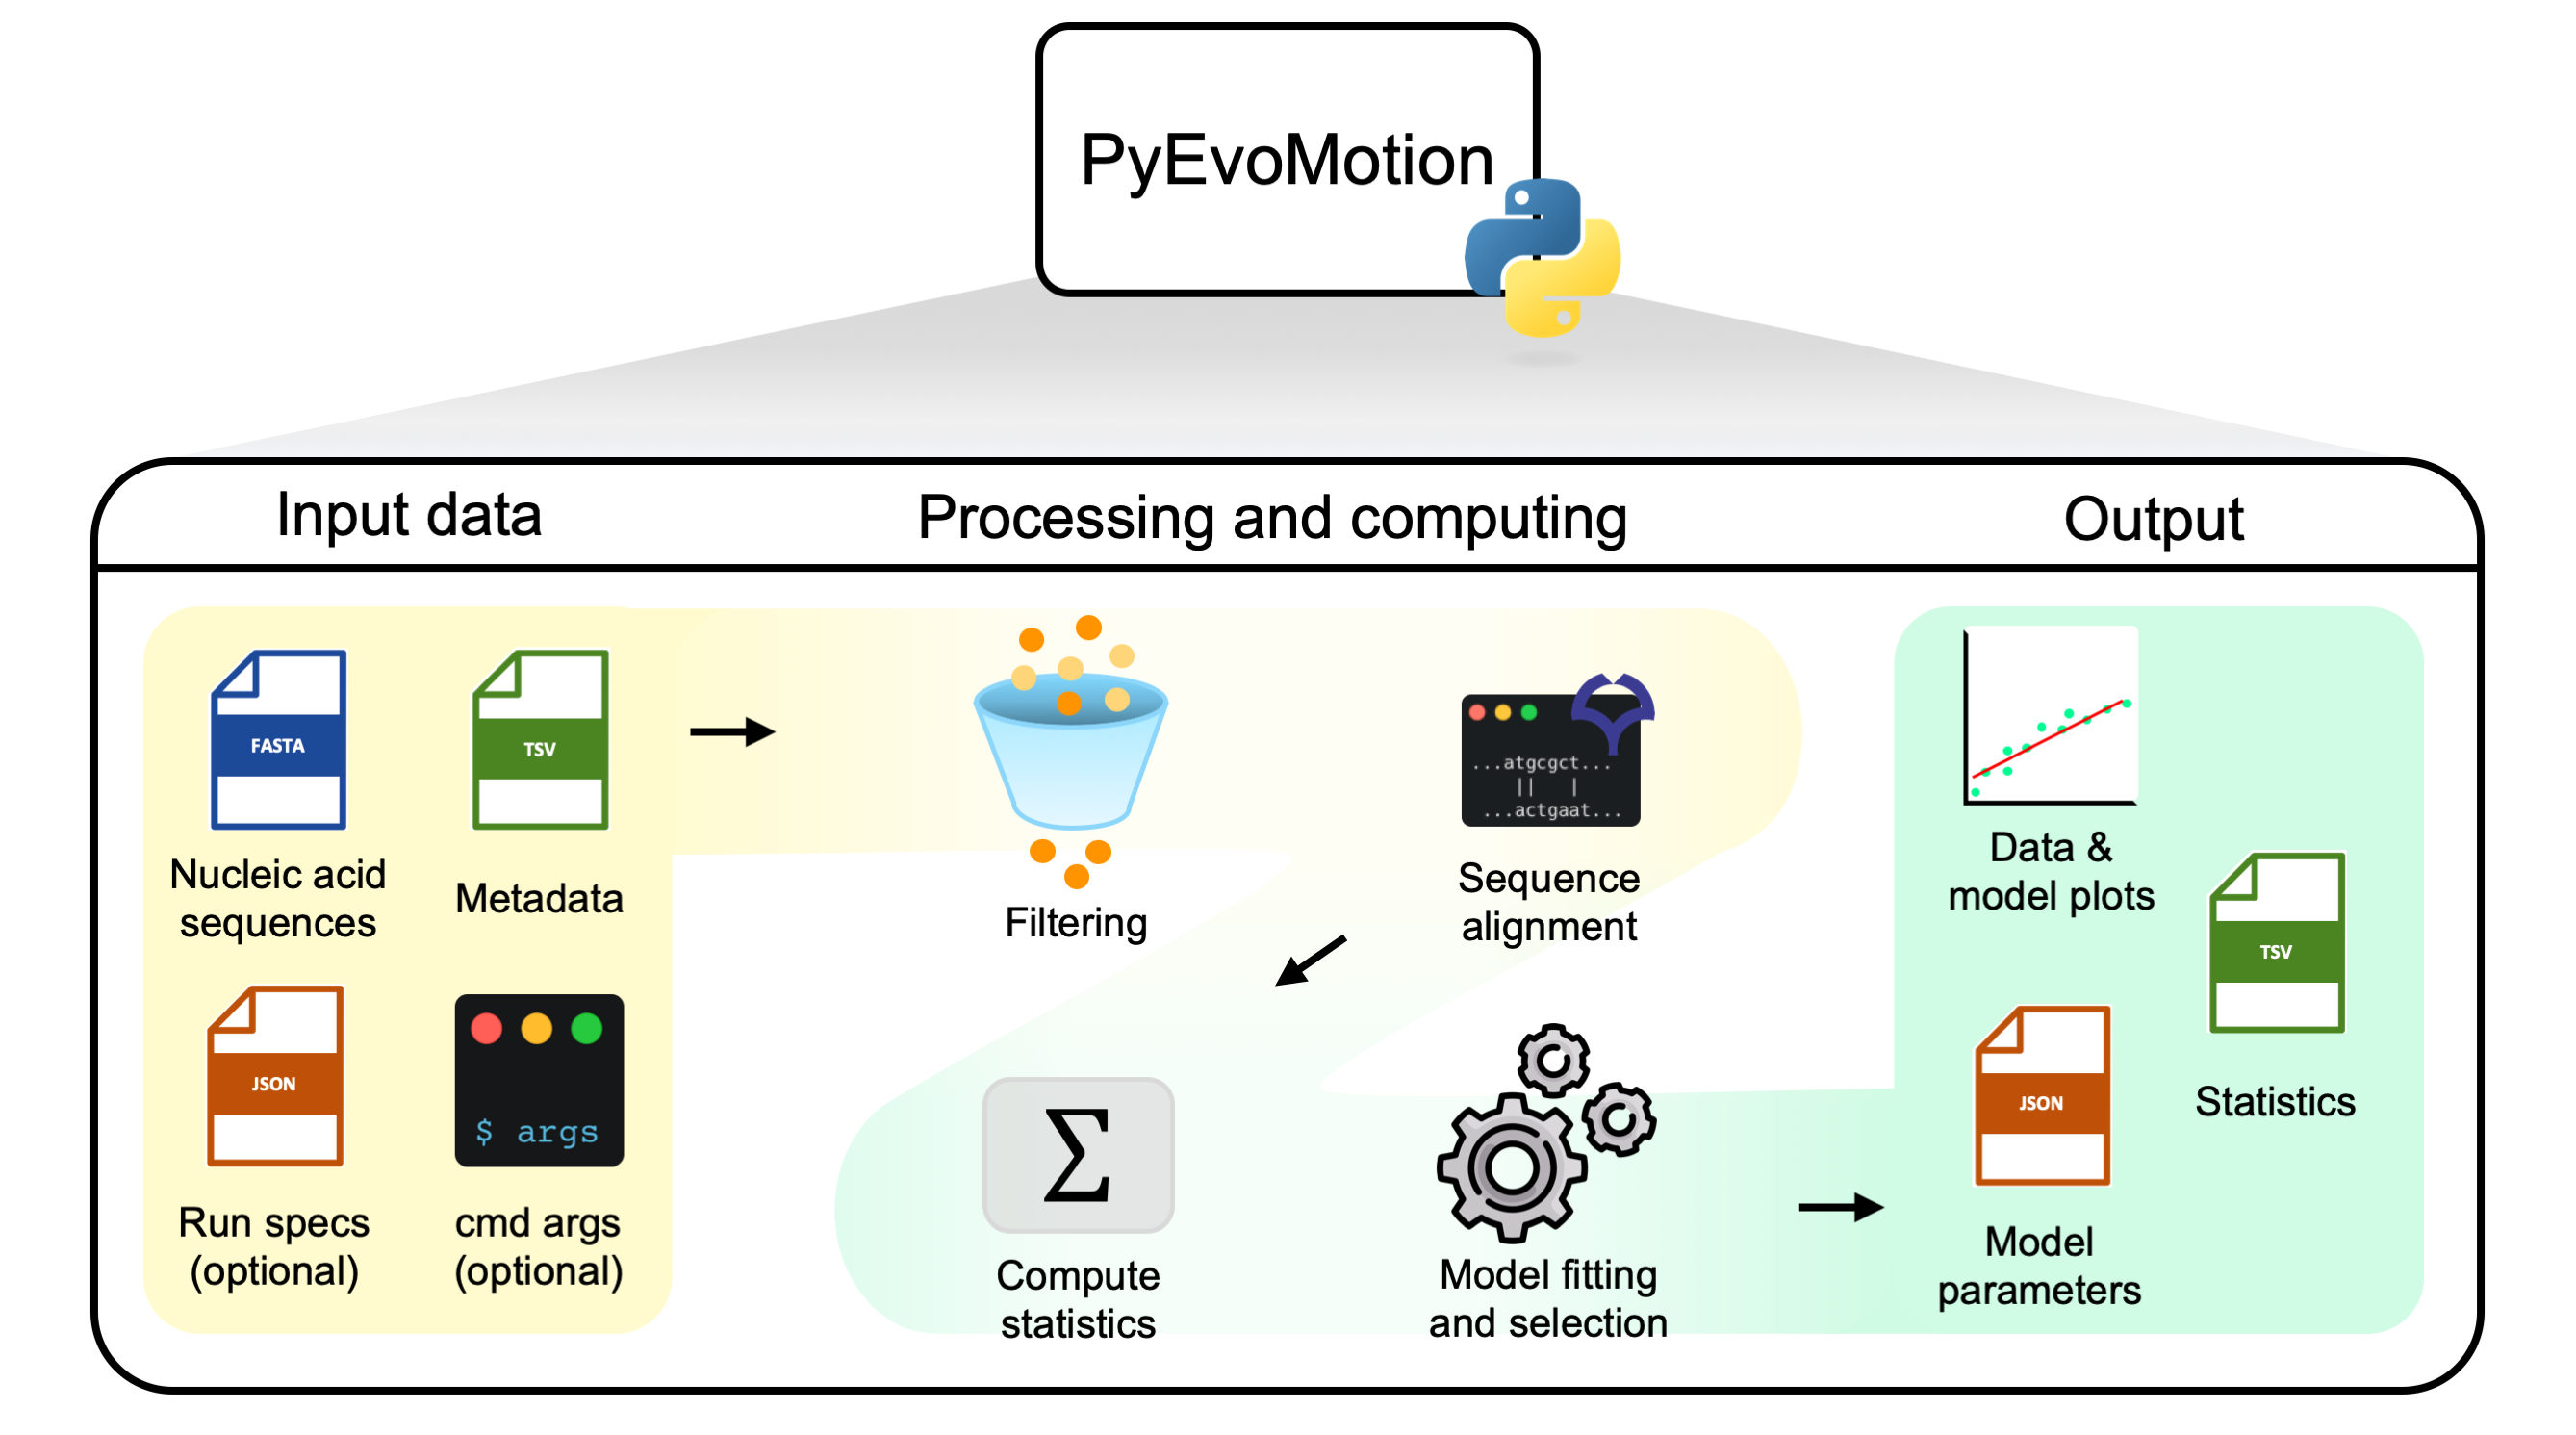
\includegraphics[trim={0 0.3cm 0 0},clip,width=0.9\textwidth]{assets/Ch3Fig1.png}
    \caption{Overview of PyEvoMotion. Mandatory input data include nucleic acid sequences (in \texttt{.fasta} format) and their corresponding metadata (in \texttt{.tsv} format). The metadata must include collection dates, as these are essential for model fitting. Output files include dynamic data representation plots and statistical parameters.}\label{fig1:pyevomotion_overview}
\end{figure*}

To begin, the temporal granularity of the analysis can be adjusted by defining the time intervals for grouping sequences and calculating statistics. By default, this interval is set to 7 d. Additionally, data filtering options are available to enhance the quality and specificity of the analysis. For instance, the length filter excludes sequences that do not meet a minimum length threshold, thereby removing low-quality genomes (unresolved bases set to a maximum of 1\% \texttt{N}). The genome position filter allows users to restrict the analysis to specific genomic regions, which is particularly useful for examining genes or genetic clusters of interest. A date range filter further refines the dataset by limiting the analysis to sequences collected within a specified timeframe.

The tool also enables users to select the types of mutations to include in the analysis. Options include: \texttt{total} (aggregating all mutations without distinction), \texttt{substitutions}, and \texttt{indels} (a combined category of insertions and deletions). These three analyses can be done at once with the option \texttt{all}. Filters based on metadata values provide additional flexibility, enabling users to focus on sequences that meet specific criteria in their non-molecular attributes.

After parsing the sequence data, the reference sequence is extracted, defined as the first entry in the \texttt{.fasta} file. Following the pre-processing step, each sequence is aligned to the reference sequence using the MAFFT algorithm \cite{katoh2013}. Below is an excerpt from PyEvoMotion's \texttt{parser.py} source file showing how MAFFT is invoked as a subprocess via the \texttt{\_run\_mafft()} class method, which directly communicates with the MAFFT executable via binary pipes. The \texttt{generate\_alignment()} class method takes two strings, invokes \texttt{\_run\_mafft()}, retrieves the aligned output binary data, and parses it via Biopython's \texttt{AlignIO}, ensuring precise, high-throughput alignment of genomic data prior to mutation detection:

\begin{lstlisting}[language=Python, caption={Calling MAFFT for sequence alignment.}]
@classmethod
def generate_alignment(cls, seq1: str, seq2: str) -> MultipleSeqAlignment:
"""
Generate a multiple sequence alignment of the input sequences using ``MAFFT``.

:param seq1: The first sequence to be aligned.
:type seq1: str
:param seq2: The second sequence to be aligned.
:type seq2: str
:return: The aligned sequences.
:rtype: ``MultipleSeqAlignment``
"""

id_1 = seq1.id
id_2 = seq2.id

if seq1.id == seq2.id:
    id_1 += "_ref"

return AlignIO.read(
    StringIO(cls._run_mafft({
        id_1: seq1.seq,
        id_2: seq2.seq
    })),
    "fasta"
)

@staticmethod
def _run_mafft(seqs_dict: dict[str,str], outformat: str = "fasta") -> str:
    """
    This function runs the MAFFT multiple sequence alignment tool on the input sequences.

    It raises an exception if the return code is not 0 (i.e. there was an error running MAFFT).

    :param seqs_dict: A dictionary containing the sequences to be aligned. The keys are the sequence
                      names and the values are the sequences.
    :type seqs_dict: dict[str,str]
    :param outformat: The output format of the alignment. Default is fasta.
    :type outformat: str
    :return: The aligned sequences as parsed from stdout. If the output format is clustal, it returns
             the alignment in clustal format; otherwise, it returns the alignment in fasta format.
    :rtype: str
    """

    cmd = ["mafft"]
    template_format = ">{}\n{}\n"

    if outformat == "clustal":
        cmd.extend(["--clustalout", "-"])

    elif outformat != "fasta":
        print(f"Unknown output format: {outformat}. Defaulting to fasta.")

    cmd.append("-")

    input_data = bytes(
        "".join(
            template_format.format(name, seq)
            for name, seq in seqs_dict.items()
        ),
        "utf-8"
    )

    ps = Popen(
        cmd,
        stdin=PIPE,
        stdout=PIPE,
        stderr=PIPE,
        shell=False
    )
    ps.stdin.write(input_data)
    ps.stdin.close()

    err = ps.stderr.read().decode("utf-8")
    out = ps.stdout.read().decode("utf-8")

    if (ps.returncode != 0) and not(ps.returncode is None):
        raise Exception(
            f"Error running MAFFT:\nStdout:\n{out}\n\nStderr:\n{err}\nReturn code: {ps.returncode}"
        )

    return out
\end{lstlisting}

Mutation events are identified from the sequence alignments and filtered based on the user-defined mutation types and genomic regions of interest. The model follows the methodology presented in Chapter \ref{ch:chapter2}, employing a stochastic differential equation that describing the accumulation of mutations over time. The simpler model assumes Gaussian white noise, leading to a scenario where the average number of mutations grows linearly and the variability scales directly with time, resembling Brownian motion. An alternative, more complex model introduces time-dependent noise characterized by a diffusion exponent, resulting in a fractional Brownian motion where the variance scales nonlinearly; both models converge when the diffusion exponent is 1, aligning with the neutral theory of molecular evolution. Statistical analyses are then conducted on the filtered mutation data for each time interval specified, computing mean and (\textit{unbiased}) variance as
%
\begin{align}
    \mu_k &= \frac{1}{N_k}\sum_{i=1}^{N_k}m_{k,i},\\
    s_k^2 &= \frac{1}{N_k-1}\sum_{i=1}^{N_k}\left(m_{k,i} - \mu_k\right)^2
\end{align}
%
where $m_{k,i}$ represents the number of mutations observed in the $i^\text{th}$ sequence during the $k^\text{th}$ time interval, while $N_k$ denotes the total number of sequences within that interval. Consequently, $\mu_k$ and $s_k^2$ correspond to the mean and variance of mutations in the $k^\text{th}$ time interval, respectively. These statistical measures serve as the basis for fitting a molecular clock model. The \texttt{compute\_stats()} method in PyEvoMotion's \texttt{core.py} source file illustrates how $\mu_k$ and $s_k^2$ are simultaneously computed for each time interval $k$.

\begin{lstlisting}[language=Python, caption={Calculation of mean and variance of mutation counts per time interval.}]
def compute_stats(self,
    DT: str,
    origin: str,
    mutation_kind: str = "all"
) -> pd.DataFrame:
    """
    Compute the length, mean and variance of the data.

    It computes the mean and variance of the data for the specified mutation kind (or kinds)
    in the specified datetime interval and origin.

    :param DT: The string datetime interval that will govern the grouping.
    :type DT: str
    :param origin: The string datetime that will be the origin of the grouping.
    :type origin: str
    :param mutation_kind: The kind of mutation to compute the statistics for. Has to be one of 
                          ``all``, ``total``, ``substitutions``, ``insertions``, ``deletions``
                          or ``indels``. Default is ``all``.
    :return: The statistics of the data.
    :rtype: ``pd.DataFrame``
    """

    grouped = self.date_grouper(self.data, DT, origin)
    levels = [
        f"number of {x}"
        for x in self._mutation_type_switch(mutation_kind)
    ]

    return pd.concat(
        (
            pd.DataFrame(self._invoke_method(grouped[levels], method))
            .rename(
                columns=lambda col: f"{method} {col}"
                if method != "size" else "size"
            )
            for method in ("mean", "var", "size")
        ),
        axis=1
    ).reset_index(level=['date'])
\end{lstlisting}

Note that the \texttt{date\_grouper()} method is a helper function that groups the data by date using \texttt{pandas}' \texttt{Grouper} class.

Furthermore, PyEvoMotion offers several configurable run-specific parameters to enhance usability and reproducibility. Users can opt to visualize the output data directly, export the plots in PDF format, save the run parameters as a \texttt{.json} file for future reference, or initialize a run using a pre-existing \texttt{.json} file. These features ensure that analyses are both customizable and reproducible, catering to diverse research needs.

\subsection{Model selection}

PyEvoMotion estimates the parameters for both models (i.e., $\kappa$ and $D$ for the null model and $\kappa$, $D$, and $\alpha$ for the challenging model) and then performs a statistical test to select the best option. For that, the calculated values of mean and variance of mutations at each time are represented, and curves are fitted.

$\kappa$ is directly the slope of the line fitted to the mean of mutations with time (this is the same for both models). The variance of mutations needs to be rescaled before fitting because the stochastic processes assume a start from the origin. Then, the initial variance is subtracted to all values ($s_k^2 - s_0^2$) and time is shifted so that $t_0=0$. In the case of the null model, $D$ is the slope of the intercept-free line fitted to the rescaled variance with time. In the case of the challenging model, a nonlinear regression with a power law relationship is used to obtain the values of $D$ and $\alpha$.

The fitting of the variance determines the choice of the molecular clock model, which is accomplished by an \textit{F}-test on the residuals of the fits using
%
\begin{equation}
    F = \frac{\frac{\text{RSS}_1-\text{RSS}_2}{p_2-p_1}}{\frac{\text{RSS}_2}{n-p_2}},
\end{equation}
%
where $\text{RSS}_1$ and $\text{RSS}_2$ are the residual sum of squares for the null and challenging models, respectively, $p_1$ and $p_2$ are the number of parameters for the null and challenging models, respectively (i.e., $p_1=1$ and $p_2=2$), and $n$ is the number of data points. The \textit{F}-test is performed at a significance level of 0.05. The snippet below, taken from PyEvoMotion's \texttt{base.py} source file, shows how the \texttt{adjust\_model()} class method implements linear (null) and a power-law (challenging) fittings to the data, and how an F-test is applied to compare the models:

\begin{lstlisting}[language=Python, caption={Linear (null) and power-law (challenging) model fitting to the data, and F-test procedure for model comparison.}]
@classmethod
def adjust_model(cls,
    x: pd.Series,
    y: pd.Series,
    name: str = None
) -> dict[str, any]:
    """Adjust a model to the data.

    :param x: The features. It is a single pandas Series.
    :type x: pd.Series
    :param y: The target. It is a single pandas Series.
    :type y: pd.Series
    :param name: The name of the data. Default is ``None``.
    :type name: str
    :return: A dictionary with the model.   
    :rtype: ``dict[str, any]``
    :raises ValueError: If the dataset is empty or full of NaN values. This may occur if the grouped
                        data contains only one entry per group, indicating that the variance cannot
                        be computed.
    """

    x,y = cls._remove_nan(x, y)

    # Raises an error if the dataset is empty at this point
    if (x.size == 0) or (y.size == 0):
        cls._check_dataset_is_not_empty(
            pd.DataFrame(),
            "Perhaps NaN appeared on all entries. Check if the grouped data contains only one
            entry per group, as this may cause NaN values when computing the variance."
        )

    # Not fitting the intercept in model 1 because data is passed scaled to the minimum
    model1 = cls.linear_regression(x, y, fit_intercept=False) 
    model2 = cls.power_law_fit(x, y)

    _, p = cls.F_test(model1, model2, y)

    if p < 0.05:
        model = model2
    else:
        model = model1

    if name:
        return {name: model}
    else:
        return model
\end{lstlisting}


The function returns a \texttt{dict} containing the the best-fit parameters and the chosen model.



\subsection{Modularity}

PyEvoMotion includes a command line interface designed for Unix-based systems. Given that most bioinformatic analyses consist of larger workflows, PyEvoMotion provides its outputs in standard formats such as \texttt{.tsv} and \texttt{.json}, which can be easily integrated into existing pipelines. The tool comes also available as a Python module, allowing users to incorporate its functionality and helper utilities into their own Python-based workflows with ease.

Interoperability limitations are minimal but not negligible, as PyEvoMotion relies heavily on MAFFT for sequence alignment. The absence of a proper foreign function interface (FFI) between PyEvoMotion and MAFFT necessitates calling the latter as a subprocess, creating a performance bottleneck. Future versions might mitigate this limitation by introducing a more Python-friendly interface.

The incorporation of alternative mathematical models is possible with little effort in PyEvoMotion due to its modular architecture. Moreover, extended versions of the tool might automatically identify different lineages when analyzing long-time datasets and use piecewise models for the mean and variance of mutations.

%VALIDATION

\section{Validation}

The utility of PyEvoMotion was validated with a real dataset containing whole-genome sequences of the SARS-CoV-2 Alpha variant from the GISAID database \cite{khare2021}. The sequences were divided into two groups based on their country of origin: the United Kingdom (UK) and the United States of America (USA). For each group, we randomly sampled 9999 sequences, kept the samples collected between October 2020 and August 2021, and analyzed the number of accumulated mutations over time with respect to the NCBI reference sequence \href{https://www.ncbi.nlm.nih.gov/nuccore/1798174254}{NC\_045512.2}. All calculations (including data parsing, filtering, sequence alignments, and model fitting) were achieved in less than 1 h in a personal computer, showing the potential scalability of the approach. 

Figure~\ref{fig2:simulation_results} shows the results. In the case of UK, the inferred evolution rate was $\hat{\kappa}=0.19$ wk${^{-1}}$, and the challenging model was the best option, inferring a diffusion coefficient of $\hat{D}=1.82$ and a diffusion exponent of $\hat{\alpha}=0.43$. In the case of USA, the inferred evolution rate was $\hat{\kappa}=0.32$ wk${^{-1}}$, and the challenging model was also selected, with inferred diffusion parameters of $\hat{D}=0.69$ and $\hat{\alpha}=0.67$.

\begin{figure}[!h]%
    \centering
    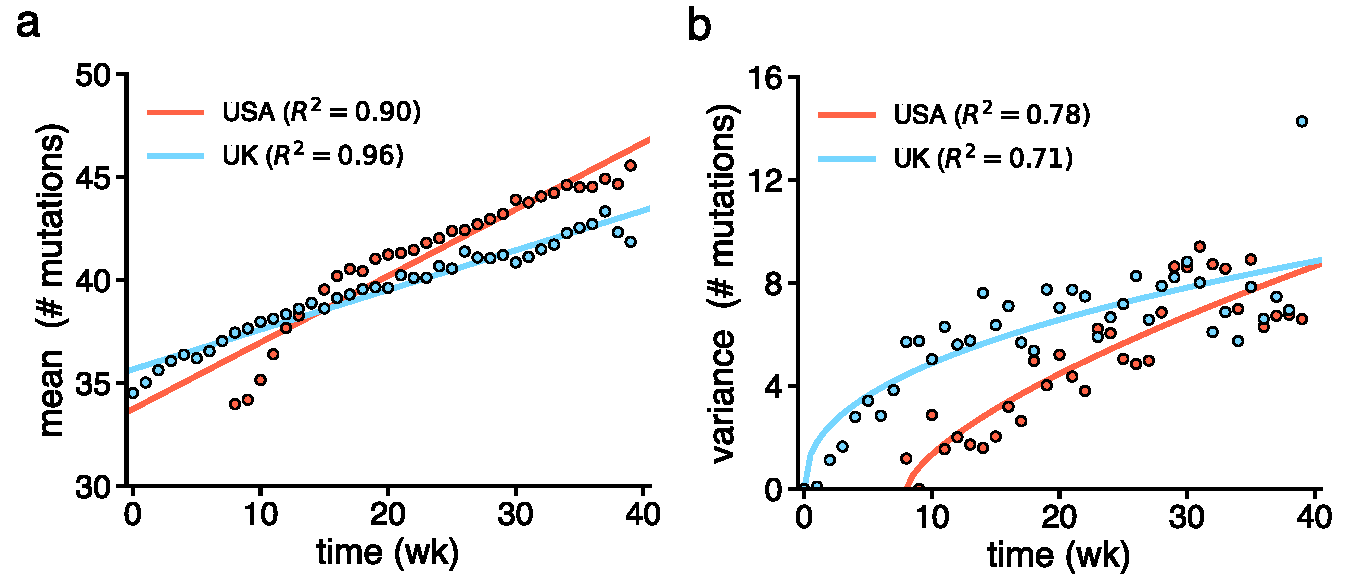
\includegraphics[width=0.95\textwidth]{assets/Ch3Fig2_horz.pdf}
    \caption{Mutational mean and variance over time in the SARS-CoV-2 Alpha variant genomes from UK and USA. a) Mean number of accumulated mutations. b) Scaled variance of the number of accumulated mutations. Points correspond to calculated values from the sequence dataset and lines to inferred molecular clock models.}\label{fig2:simulation_results}
\end{figure}

%CONCLUSIONS

\section{Conclusions}

Here, we present a high-throughput data-processing, open-source, user-friendly software, called PyEvoMotion, to study evolutionary motions under a statistical perspective provided a collection of genomic sequences. PyEvoMotion is designed to be flexible and customizable, offering a wide range of options for data analysis. Such statistical analysis is complementary to phylogenetic tree reconstructions and molecular assays that measure the impact of key mutations \cite{Mlcochova2021}. 

Nonetheless, our work presents some limitations. In the models, the evolution rate is assumed constant, despite it can vary with time if lineages with higher fitness emerge and even be non-linear if adaptation is the dominant process \cite{tenaillon2016}. This would require applying the date filter to limit the analysis to a subset of sequences, as we did to obtain the results shown in Figure~\ref{fig2:simulation_results}. Moreover, this statistical approach fails to provide meaningful insight if the collection of sequences is not sufficiently large and does not span in time.

In addition to virus evolution, PyEvoMotion might be used to study the tempo and mode of accumulation of mutations in bacteria \cite{tenaillon2016} or in cancer cells \cite{borgsmuller2023}. Understanding the dynamics of these rapidly evolving biological entities might have biomedical implications.

\section*{Data availability}
The open source software is available on GitHub at \href{https://github.com/luksgrin/PyEvoMotion}{\texttt{https://github.com/luksgrin/PyEvoMotion}} and on SourceForge at \href{https://sourceforge.net/projects/pyevomotion}{\texttt{https://sourceforge.net/projects/pyevomotion}}. Genomic data used in the validation were extracted from the GISAID database (\href{https://www.gisaid.org}{\texttt{https://www.gisaid.org}}) and are available on SourceForge.

\vfill

\pagebreak

\bibliographystyle{assets/rodrigostyle}
\bibliography{references/chapter3references}
\vfill
\pagebreak ~

% Paper 3
\chapter{Deciphering microscopic drivers of viral genome-scale molecular clock dynamics}

\begin{flushright}
    \textit{Nothing in biology makes sense except in the light of evolution.}\\
    --- Theodosius Dobzhansky
\end{flushright}

\vspace{1cm}

\noindent This work has been sent to a peer-reviewed journal.\\

\noindent \textbf{Goiriz L}, Rodrigo G. (2025) {Deciphering microscopic drivers of viral genome-scale molecular clock dynamics}. \textit{Under review}.\\

\noindent In this work, I performed all the data analysis and figures. The results were discussed with GR. GR designed the research.

\vfill

\pagebreak

\sloppy

\section{Introduction}
Viruses, and in particular RNA viruses, with their short generation times and high mutation rates, offer a unique window into the dynamics of evolution \cite{elena2007virus}. Unlike in many organisms, the mutation accumulation process in viruses can be observed in real time, making them ideal systems for studying the mechanisms that drive genetic variation. By analyzing viral genomes, we can test evolutionary theories, such as neutral theory \cite{gojobori1990molecular} or lethal mutagenesis \cite{crotty2001rna}, we can track how mutations spread through populations \cite{kraemer2021spatiotemporal,viana2022rapid}, which results in a critical tool in epidemiology to propose suitable interventions, and we can ultimately assess how selection, drift, and recombination shape genetic diversity \cite{nelson2006stochastic,tully2009shifts}. However, viruses do not evolve uniformly across their genomes. They contain several genes coding for different types of proteins (e.g., structural and non-structural), each subject to singular selection pressures that shape its evolution rate and variability \cite{gray2011mode}. For example, genes encoding instrumental proteins to generate progeny [e.g., capsid or RNA-dependent RNA polymerase (RdRp)] tend to evolve more slowly due to strong purifying selection, while genes encoding proteins involved in direct interactions with host cell elements (e.g., glycoproteins with receptor-binding domains) are usually subject to positive selection \cite{kistler2022rapid}. In this regard, further research is needed to determine the precise contribution of each gene, which may additionally change with time, to the evolution of a virus as a whole entity.

Evolutionary processes are often described using stochastic models that assume regularity in the accumulation of genetic changes. The molecular clock hypothesis is a traditional theoretical framework derived from neutral theory that has provided foundational insights into diversification by relying on the assumption that mutations accumulate at a relatively constant rate over time and that the extent of variability in a population follows a Poisson distribution \cite{kimura1987molecular,kumar2005molecular}. Despite the wide application of this model, virus evolution can deviate from its predictions due to factors such as transmission bottlenecks, host immune pressures (e.g., vaccination), and environmental changes \cite{jenkins2002rates}. In this regard, relaxed molecular clock descriptions have been developed to allow evolution rates to vary among phylogenetic tree branches, thereby accommodating the potential effects of external factors \cite{drummond2006relaxed}. In these models, however, variation is always driven by delta-correlated (white) Gaussian noise to end with Poissonian statistics. We can then consider that each gene from a virus evolves at a given rate displaying a distinctive level of variation and that the integration of the different dynamics results into the observed evolutionary movement of the virus \cite{neher2022contributions}. Disentangling the overlooked statistical properties that characterize such individual dynamics is important for a fundamental understanding of the process and requires further introspective analysis of high-throughput sequencing data. 

The global public health crisis provoked by the emergence of severe acute respiratory syndrome coronavirus 2 (SARS-CoV-2; \cite{wu2020new}) prompted the implementation of genomic surveillance programs. It is therefore appealing to focus the study on this RNA virus to take advantage of the resulting database with millions of whole genome sequences. Notably, such efforts facilitated the detection of novel variants of concern \cite{viana2022rapid}, as well as the spatiotemporal monitoring of the impact of introduction and superspreading events \cite{kraemer2021spatiotemporal,lemieux2021phylogenetic}. They have also allowed the quantification of the interplay between adaptation, neutrality, and purifying selection during virus evolution in nature at an unprecedented resolution \cite{neher2022contributions,markov2023evolution}. In particular, it has been shown that rapid bursts of adaptation were followed by phases of slow evolution in which purifying selection predominated. Moreover, we have pointed out that each variant evolved at a different rate and that the observed genetic variability is compatible with a stochastic anomalous diffusion process (viz., with time-dependent Gaussian noise) distinctively parameterized in each case \cite{goiriz2023variant}. This indicates deviations from Poissonian statistics and highlights evolutionary constraints associated with each genotype. Notwithstanding, the mechanisms underlying this anomalous diffusion behavior remain unknown. 

In this work, we analyze the gene-level mutational dynamics of SARS-CoV-2 to determine how microscopic contributions shape macroscopic evolutionary trends. For that, we focus on the different within-variant evolution phases and quantify for each gene the process of mutation accumulation and the generation of variability. More specifically, we calculate the mean number of accumulated mutations, the mutational variance of the population, and the frequency of each mutation to provide a comprehensive evolutionary picture for each of the 27 genes of SARS-CoV-2 \cite{yang2021structural} (ORF3b and ORF9c were discarded in our study). We aim to identify whether specific genes show deviations from the classical molecular clock predictions and how these local effects drive the anomalous diffusion behavior reported at the genome-scale level. Unraveling these complexities might also enhance our ability to predict virus evolution \cite{rouzine2001transition}, with implications in epidemiology. To effectively process a massive number of genomic sequences, we here follow a statistical approach \cite{obermeyer2022analysis,goiriz2023variant}, examining population genetic compositions over time rather than reconstructing phylogenetic trees from genetic variation. Conventional phylogenetic methods \cite{bouckaert2014beast} show great utility to track pathogen evolution in public health crisis scenarios in order to e.g. identify mutations that increase fitness and to trace transmission routes (especially when mobility data are aggregated; \cite{kraemer2021spatiotemporal}). However, they do not directly follow the genetic shaping of the population through characteristic statistical parameters (moments, frequencies) and highly depend on proper prior selection; in addition to struggling with scalability due to an excessive computational demand, thereby becoming unpractical or requiring approximations when dealing with a vast number of sequences \cite{demaio2023maximum}. Through this top-down approach from large empirical observations, we seek to refine probabilistic models of viral genome evolution under the molecular clock prism and further appreciate the complexity of the mutation-selection process in infectious agents circulating in nature.

\section{Results}
We implemented a simple-method computational pipeline to process the massive number of available SARS-CoV-2 whole genome sequences and extract time-dependent statistical parameters characterizing the evolutionary trajectory of the virus. We mainly focused our analysis on the United Kingdom (UK) during the first 120 weeks of pandemic, because a strong genomic surveillance program was implemented in this geographic region at that time \cite{coguk2020integrated}. After curating the available dataset to remove poor-quality, non-date-annotated, and outlier items, we obtained 1.87 million high-quality genome sequences. With respect to the reference sequence from Wuhan (China), we identified 108,347 different mutations distributed throughout the virus genome during those 120 weeks, including substitutions, insertions, and deletions (indels). During this period, new variants of concern emerged (Alpha, Delta, and Omicron), which invaded the population one after another as a consequence of acquiring distinct mutations that enhanced their transmissibility and immune evasion capabilities \cite{tao2021biological}.

A temporal representation of the mean number of accumulated mutations by gene pointed out to PLpro (encoding a protease for polyprotein processing), RdRp (encoding the replicase), S (encoding the spike protein for viral entry), and N (encoding the nucleocapsid) as the most evolved genes since the pandemic origin (\textbf{Fig. \ref{fig:fig4.1}a}). ORF9b also appeared as evolved as it overlaps with N \cite{yang2021structural}. With the emergence of Omicron, S separated from the rest of genes in terms of divergence. Other genes started to evolve with the emergence of variants, such as ORF8 with Alpha, nsp4, nsp6, and ORF7a with Delta, and M and ORF6 with Omicron. In addition, a representation of the dispersion index of the virus population by gene, calculated as the ratio between the mutational variance and mean \cite{gillespie1984molecular}, yielded a mosaic-like picture (\textbf{Fig. \ref{fig:fig4.1}b}).

\begin{figure}[ht!]
    \centering
    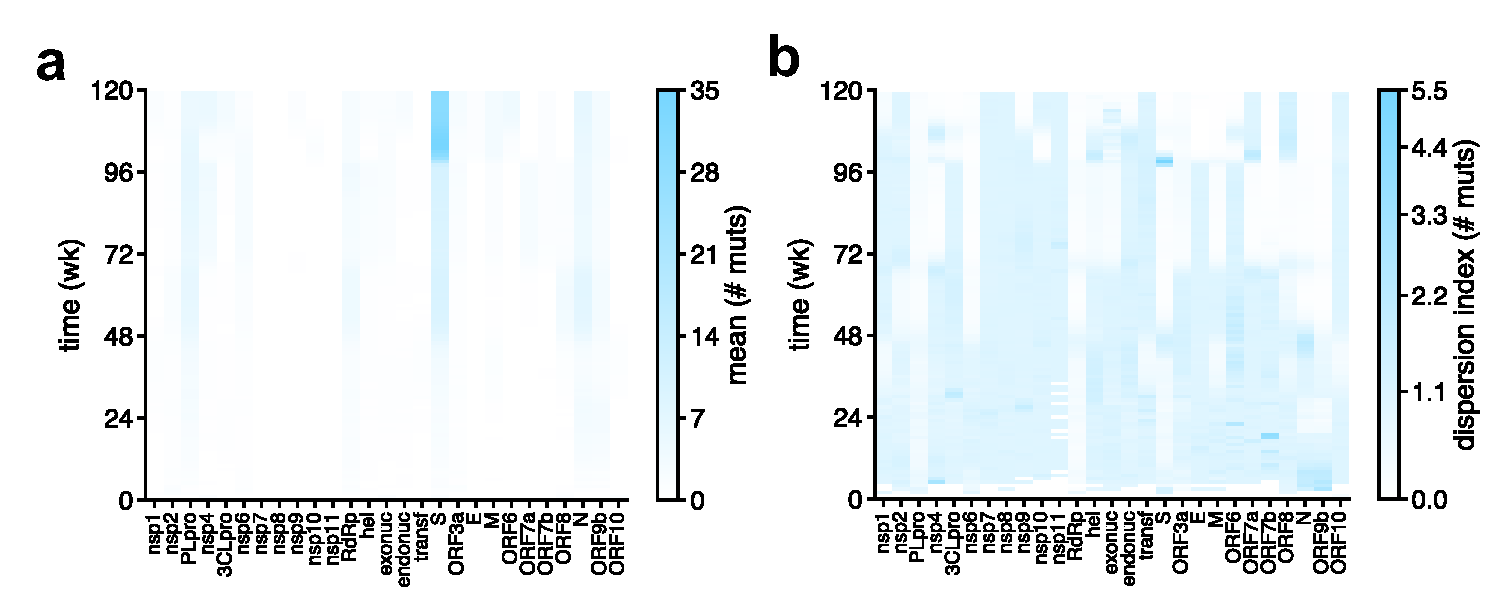
\includegraphics[width=\linewidth]{assets/Ch4Fig1.pdf}
    \caption{a) Time-course of the mean number of accumulated mutations in each gene of the SARS-CoV-2 genome, including substitutions and indels (with respect to the reference sequence from Wuhan; data from the UK). Heatmap colored using a linear scale. b) Time-course of the dispersion index (variance-to-mean ratio) of accumulated mutations in each gene of the SARS-CoV-2 genome. Heatmap colored using an inverse hyperbolic sine scale.}\label{fig:fig4.1}
\end{figure}

Non-monotonous variations in dispersion index indicate complex evolutionary trajectories, beyond deviations from Poissonian statistics. The highest genetic dispersion occurred in S with the invasion of Omicron BA.1, in agreement with multiple introductions of different sublineages in the UK \cite{tsui2023genomic}. Despite having significant evolution rate, RdRp continuously displayed reduced levels of dispersion, which could be a signature of purifying selection in order to maintain an efficient viral replication. Moreover, during the period in which Delta was the dominant variant, the dispersion in several genes was substantially low, reflecting a founder effect.

Overall, SARS-CoV-2 evolved through adaptation in a punctuated manner by accumulating non-synonymous mutations (\textbf{Fig. \ref{fig:fig4.2}a}). However, while the emergence and invasion of Alpha and Omicron BA.1 entailed bursts of non-synonymous mutations (at weeks 44 and 99, respectively), with Delta the number of non-synonymous substitutions was roughly maintained and the synonymous substitutions significantly decreased (at week 66). The dispersion index peaks ($>$ 1) clearly supported this view of the transitions (\textbf{Fig. \ref{fig:fig4.2}b}; see also the dispersion index calculated for genes encoding structural and non-structural proteins in \textbf{Fig. \ref{fig:fig4.2}c}). This is in tune with an independent emergence of Alpha and Delta in late 2020, noting that Delta first spread in India and then was introduced in the UK. Inferences of the evolution rates by gene and mutation type revealed the inclination of S, E, N, ORF7a, and exonuc to incorporate non-synonymous changes (a signature suggesting adaptation). For example, mutations H655Y and T95I in S, T9I in E, and P13L in N have been highly ranked in terms of their positive effect on viral fitness \cite{obermeyer2022analysis}. Inferences also showed that nsp9 and nsp10 preferentially accumulated synonymous mutations (a signature of purifying selection), and that nsp6 and ORF8 preferentially accumulated indels (\textbf{Fig. \ref{fig:fig4.2}d}). It has been proposed that ORF8 knockout contributes to increase viral fitness, although this may depend on the genetic background \cite{wagner2024positive}.

\begin{figure}[ht!]
    \centering
    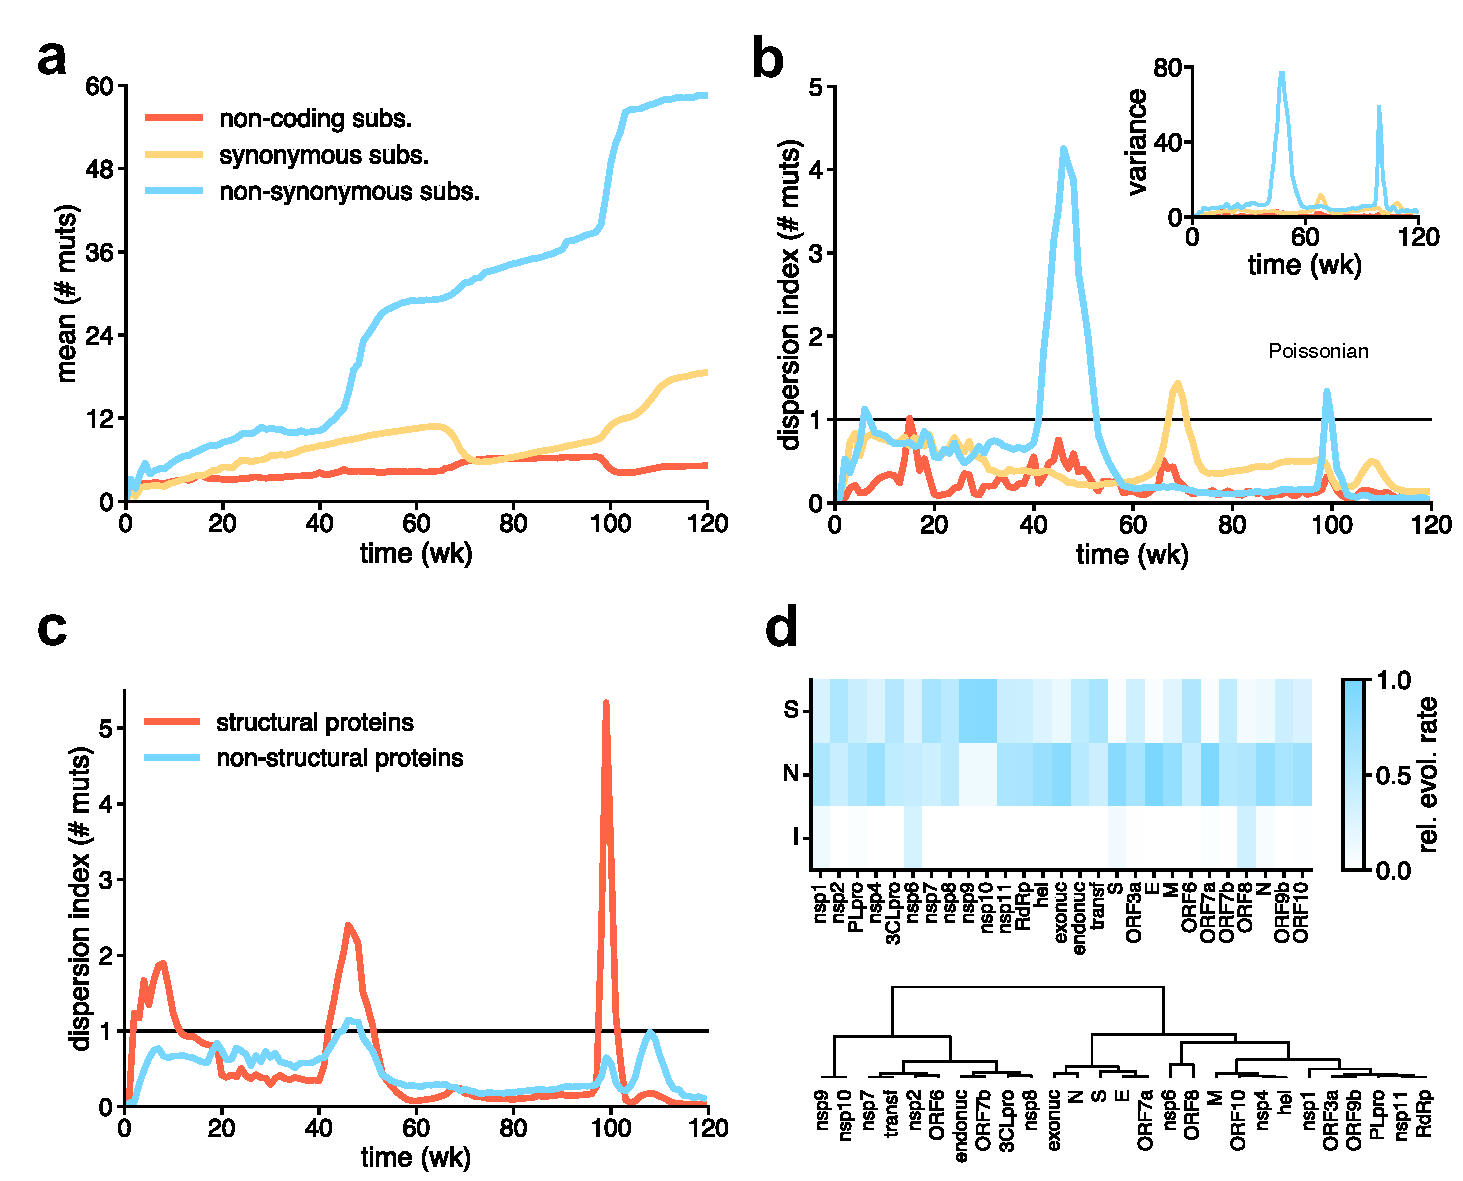
\includegraphics[width=\linewidth]{assets/Ch4Fig2.pdf}
    \caption{a) Time-course of the mean number of non-coding, synonymous, and non-synonymous substitutions. b) Time-course of the dispersion index of non-coding, synonymous, and non-synonymous substitutions. Inset, variance of substitutions with time. c) Time-course of the dispersion index in genes encoding structural and non-structural proteins. d) Inferred relative evolution rate for each gene and mutation type [synonymous substitutions (S), non-synonymous substitutions (N), and indels (I)]. Bottom, hierarchical clustering of genes.}\label{fig:fig4.2}
\end{figure}

We also analyzed the number of accumulated mutations in each gene from datasets of other countries [viz., the United States of America (USA), Spain, India, South Africa, and Japan]. Comparing the inferred evolution rates, we found similar dynamics overall (\textbf{Fig. \ref{fig:fig4.3}a}). Furthermore, we observed an interesting relationship between mutational mean and variance at particular times strictly dominated by a single variant in the UK. Considering the absolute number of mutations in each gene, Poissonian statistics hold in the case of low mutational load, being sub-Poissonian otherwise. Nevertheless, all late-stage mutational distributions get closer to the Poissonian regime by accounting for the founder effect (\textbf{Fig. \ref{fig:fig4.3}b}). Together, these results highlight the non-homogeneous genetic modulation of the virus and encourage further investigation at the variant level to completely decipher the evolutionary role of each gene.

\begin{figure}[ht!]
    \centering
    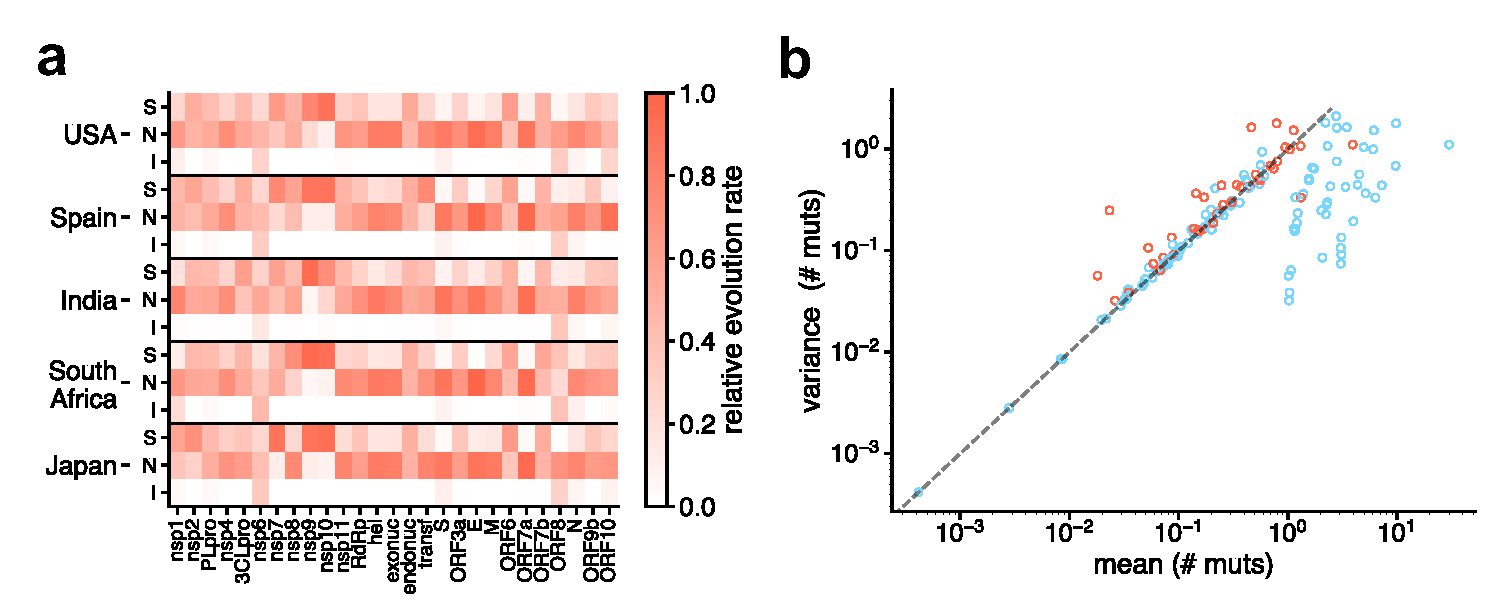
\includegraphics[width=\linewidth]{assets/Ch4Fig3.pdf}
    \caption{a) Inferred relative evolution rate for each gene and mutation type in different countries. b) Scatter plot between mean and variance in each gene at different weeks (1, 30, 60, 90, and 119). Dashed line corresponds to equal variance and mean (i.e., Poissonian regime).}\label{fig:fig4.3}
\end{figure}

According to our previous work, the whole genome of the virus accrued mutations at a nearly linear rate when particularizing for a given variant after emergence \cite{goiriz2023variant}, as predicted by the traditional molecular clock model. However, by analyzing the mean mutational load of each gene, we observed widely different dynamics (note that to ensure high statistical power, we restricted the analysis to the time window in which each variant represented at least 10\% of the population). While linear trends could be observed in various cases, we also found genes displaying highly non-linear mutation accumulation and even genes with non-monotonous and decreasing trends (\textbf{Fig. \ref{fig:fig4.4}}). The analysis of the genetic variability observed in the populations of the distinct variants also revealed intriguing microscopic aspects of the evolutionary movement of the virus, noting that an empirical model with a power law relationship between time and variance better explains the genomic data \cite{goiriz2023variant}. As in the case of the mean, non-linear, non-monotonous, and decreasing trends were found when computing the variance of the number of mutations for the different genes (\textbf{Fig. \ref{fig:fig4.5}}).

\begin{figure}[ht!]
    \centering
    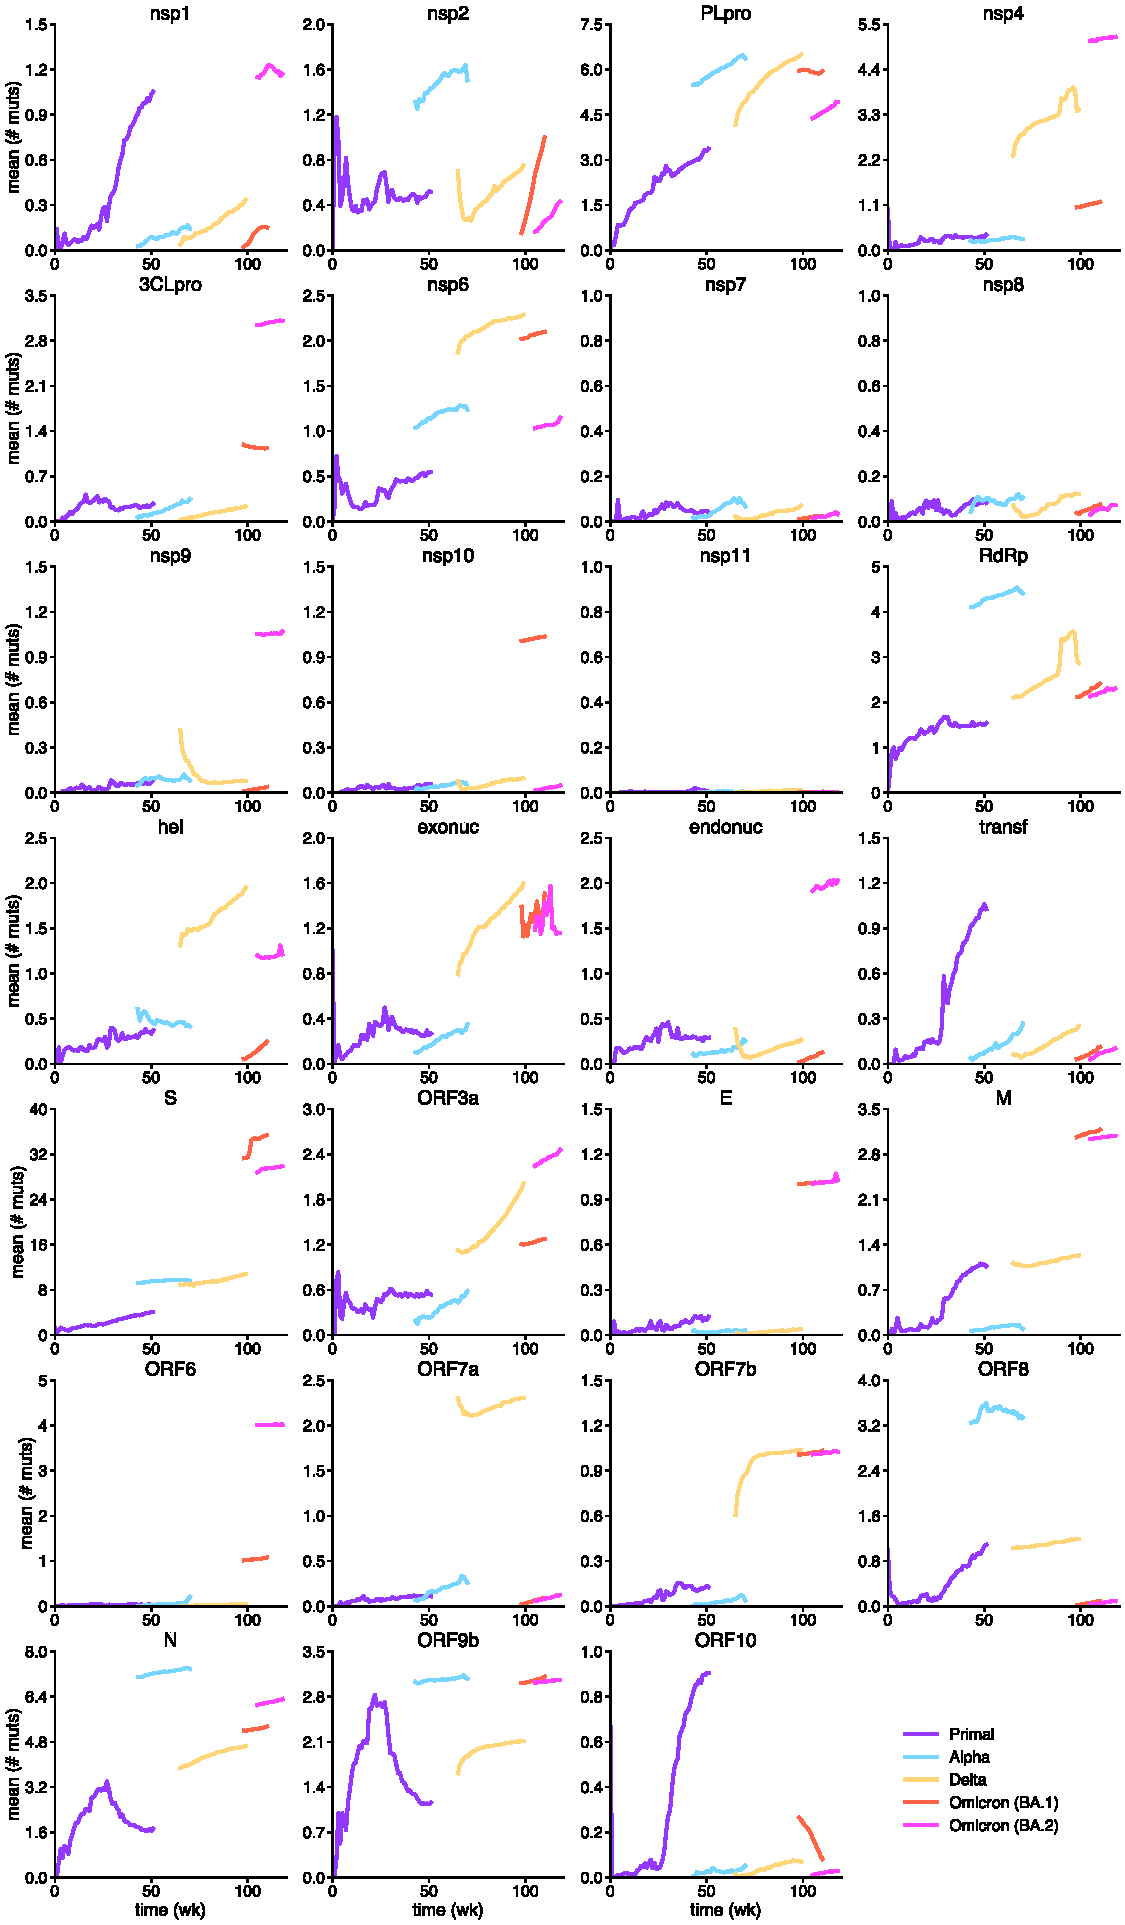
\includegraphics[width=0.7375\linewidth]{assets/Ch4Fig4.pdf}
    \caption{Gene-by-gene analysis of the variant-specific evolutionary trajectory of SARS-CoV-2. Time-course of the mean number of accumulated mutations in each gene of the SARS-CoV-2 genome and for each variant (Primal, Alpha, Delta, and Omicron BA.1 and BA.2). Mutations included substitutions and indels (with respect to the reference sequence from Wuhan; data from the UK). Analysis restricted to the time period in which the population frequencies of the variants were at least 10\%.}\label{fig:fig4.4}
\end{figure}

\begin{figure}[ht!]
    \centering
    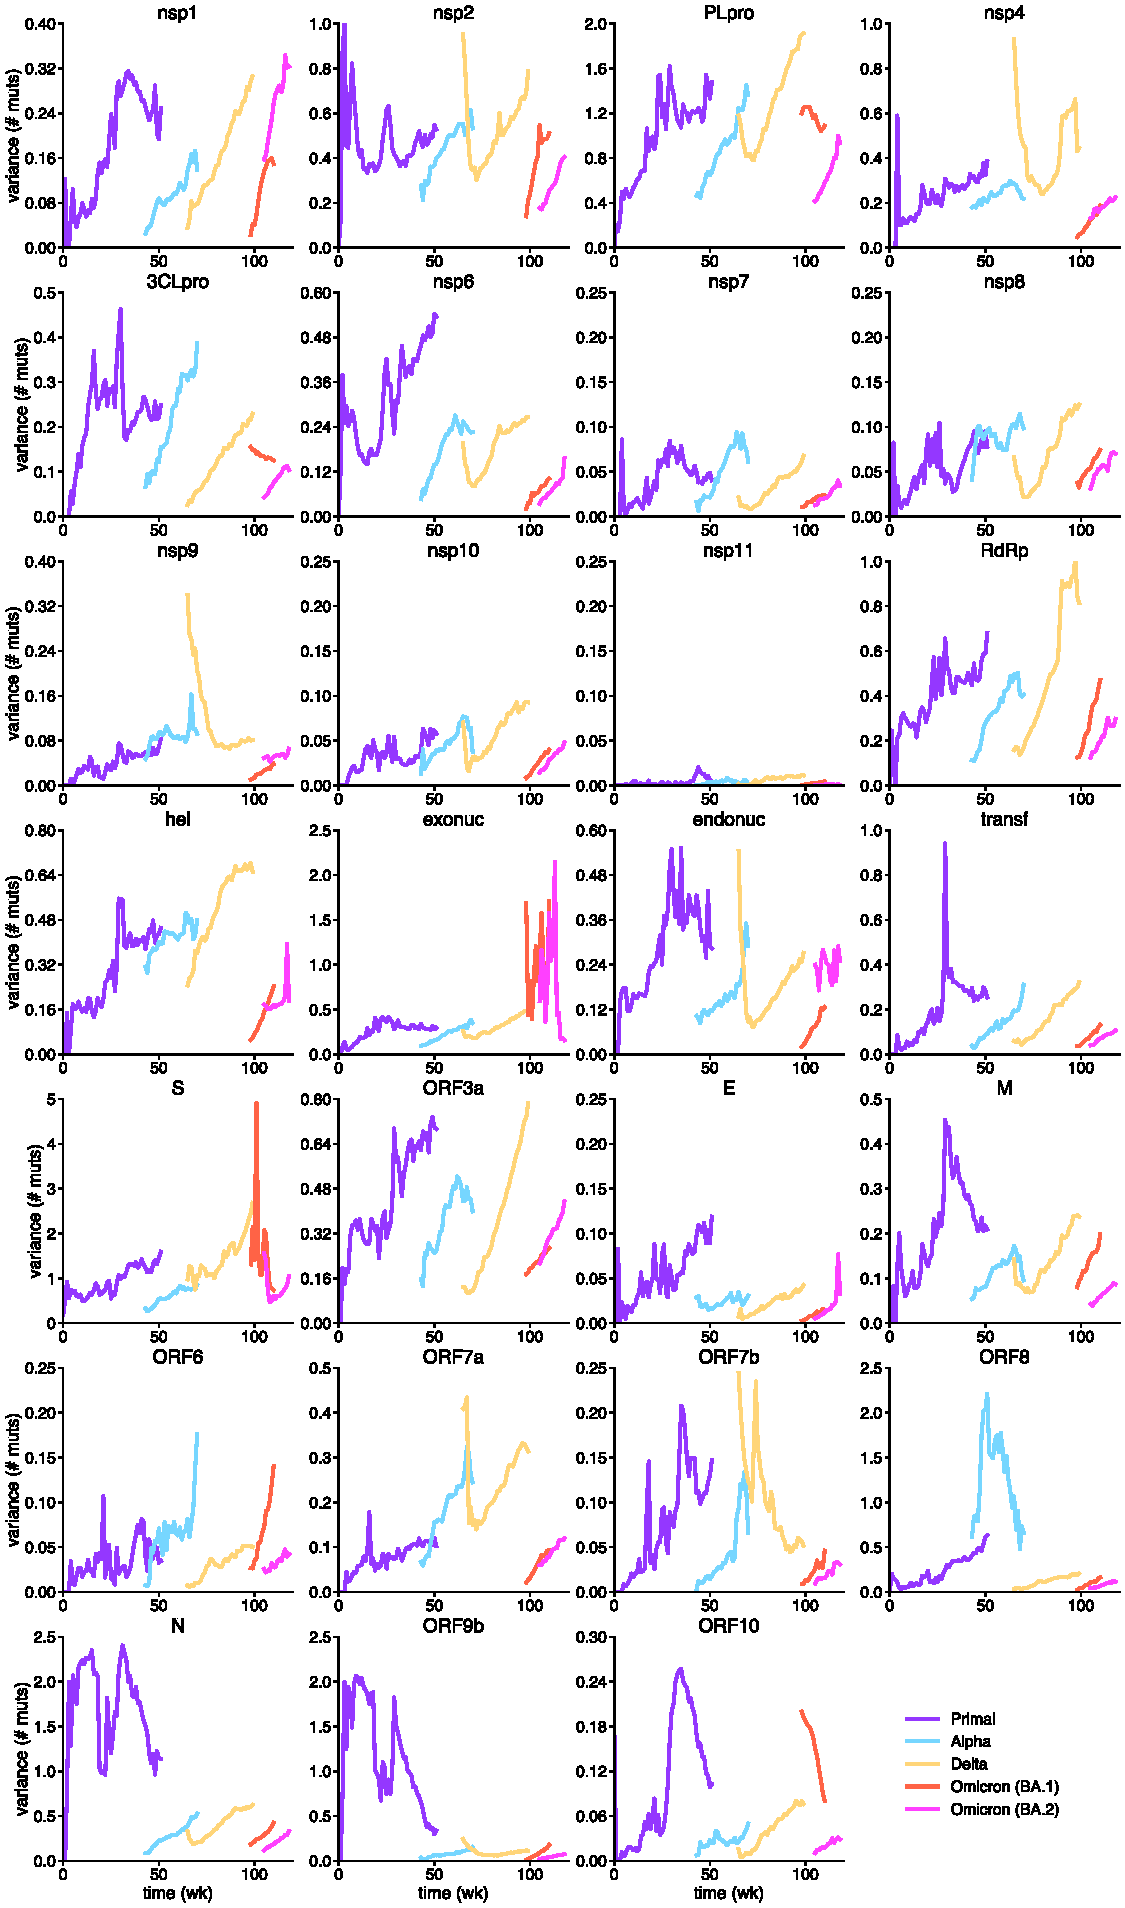
\includegraphics[width=0.7375\linewidth]{assets/Ch4Fig5.pdf}
    \caption{Gene-by-gene analysis of the variant-specific evolutionary diffusion of SARS-CoV-2. Time-course of the variance of accumulated mutations in each gene of the SARS-CoV-2 genome and for each variant (Primal, Alpha, Delta, and Omicron BA.1 and BA.2). Mutations included substitutions and indels (with respect to the reference sequence from Wuhan; data from the UK). Analysis restricted to the time period in which the population frequencies of the variants were at least 10\%.}\label{fig:fig4.5}
\end{figure}

\vfill
\pagebreak

\section{Conclusions}
Here, we have examined the microscopic factors that drive the genome-scale molecular clock dynamics of SARS-CoV-2, capitalizing on the unprecedented quantity of high-resolution sequencing data. By dissecting the virus' genome into its constituent genes, we uncovered strong non-uniformity in the patterns of mutation accumulation, highlighting the mosaic-like nature of SARS-CoV-2 evolution. Although global, genome-wide analyses reveal an overall quasi-linear accumulation of mutations at the variant level, consistent with certain predictions of the molecular clock framework, gene-level investigations reveal that specific loci often deviate from canonical Poissonian behaviors. Critically, some genes displayed highly non-monotonous or even decreasing trends in both mean mutational load and variance, underscoring the importance of local selection pressures, functional constraints, and founder effects in shaping evolutionary outcomes.

Our findings show that genes encoding essential viral functions, such as those involved in replication (RdRp) or structural integrity (N, S, and M), exhibit distinct evolutionary trajectories, reflecting a delicate balance between purifying selection and bursts of adaptive mutations. This dynamic is further evidenced by the shifts in dispersion indices through time: while some genes remain under tightly constrained evolution due to critical functional requirements (e.g., RdRp), others, particularly those facing strong interactions with host immune elements, undergo episodic bursts of adaptation (e.g., S). For instance, the non-monotonous or even decreasing mutation trajectories observed in certain genes likely result from transient selective sweeps or founder events that reset local genetic diversity, illustrating how chance transmission bottlenecks can temporarily invert or slow evolutionary trends at specific loci \cite{markov2023evolution}. Importantly, our approach leverages a statistical “top-down” perspective on the data and circumvents the computational hurdles frequently associated with large-scale phylogenetic reconstructions, thereby enabling the detection of subtle gene-level signatures of sub- or super-Poissonian mutation dynamics.

In sum, the gene-by-gene exploration presented here deepens our understanding of viral population diversification and its relationship to the classical molecular clock hypothesis. While certain global properties of SARS-CoV-2 evolution can be adequately captured by simple stochastic models, the local deviations at specific genes illustrate that the true evolutionary landscape is more intricate, non-uniform and punctuated: periods of quasi-clock-like, gradual change are interspersed with bursts of accelerated evolution when selective pressures shift \cite{tay2022}.Future research that integrates functional assays, structural studies, and comparative genomics across closely related coronaviruses will help elucidate the mechanisms behind these locus-specific dynamics and further enhance our ability to forecast evolutionary trajectories relevant to public health interventions.
\section{Materials and Methods}
\subsection{Genomic data}
The nucleotide sequences of the SARS-CoV-2 genomes used in this study were retrieved from the GISAID database \cite{khare2021gisaid}. As of May 2022, more than 10 million sequences and the corresponding metadata were downloaded. In this work, only sequences originating from the UK, the USA, Spain, India, South Africa, and Japan were included in the analysis due to their overall quality and to have a broad geographic coverage (the main analysis, however, was done with the data from the UK). The nucleotide sequences of the SARS-CoV-2 genomes were aligned against the NCBI reference genome \texttt{NC\_045512.2} (\texttt{hCoV-19/Wuhan/IVDC-HB-01/2019}, GISAID accession \texttt{EPI\_ISL\_402119}) using Multiple Alignment using Fast Fourier Transform (MAFFT; \cite{katoh2002mafft}). The results were collected in Clustal format. For each sequence in the dataset, the number of mutations (substitutions and indels) with respect to the reference genome were counted. This information was retrieved from the MAFFT output alignments. Additionally, the sequence collection dates and Pangolin lineages (to assign the variant names) were retrieved from the metadata. Next, a filtering step was applied to discard sequences without recorded dates, sequences of poor quality (e.g., whose size was below 25 kb), sequences isolated from non-human hosts, duplicated entries, and outlier sequences (which could originate from incorrect date annotations, aberrant evolutionary trajectories, or sudden point introductions; \cite{goiriz2023variant}). 

\subsection{Statistical calculations}

The genome sequences of the resulting dataset were grouped by weeks. For each week, the mean number of accumulated mutations of the viral population, the variance of the accumulated mutations, and the dispersion index (defined as the ratio between variance and mean) were computed. Protein-coding regions were translated to calculate the degree of heterogeneity in the population as the mean Hamming distance between all amino acid sequence pairs, as well as the frequency of each different mutation (non-synonymous substitutions and indels). Moreover, the mean dN/dS ratio was calculated to get an estimate of natural selection, relying on the method proposed by \cite{goldman1994codon}.

The dynamic analysis was performed by accounting for the different types of mutations accumulated in the whole genome and in each gene of the virus (27 genes were considered: nsp1, nsp2, PLpro, nsp4, 3CLpro, nsp6, nsp7, nsp8, nsp9, nsp10, nsp11, RdRp, hel, exonuc, endonuc, transf, S, ORF3a, E, M, ORF6, ORF7a, ORF7b, ORF8, N, ORF9b, and ORF10, discarding ORF3b and ORF9c; \cite{yang2021structural}). Variant-specific analyses were also performed in which only the sequences assigned to a given variant were considered \cite{neher2022contributions,goiriz2023variant}. Here, Primal (the primary lineage from the reference sequence), Alpha, Delta, and Omicron (BA.1 and BA.2) were the variants of study. Only time periods during which a given variant represented at least 10\% of the population were considered, thereby ensuring reliable statistical calculations. Mutations were classified by type (substitutions and indels), and among substitutions we distinguished non-coding substitutions (i.e., substitutions occurring in non-coding regions), synonymous substitutions, and non-synonymous substitutions. Mutations were also classified as those affecting genes coding for structural (S, E, M, and N) and non-structural proteins. The evolution rate for each gene and mutation type was estimated as the slope of the best-fit linear regression model applied to the temporal count of mutations (synonymous and non-synonymous substitutions and indels). To facilitate comparisons across genes regarding the mutation types preferentially accumulated over time, these slopes were normalized (viz., dividing by the sum of evolution rates for each mutation type). All data analyses were performed in Python using the libraries Pandas (\url{https://pandas.pydata.org}), NumPy (\url{https://numpy.org}), SciPy (\url{https://scipy.org}), Scikit-learn (\url{https://scikit-learn.org}), and Biopython (\url{https://biopython.org}) \cite{mckinney2012python,cock2009biopython}.

\vfill

\pagebreak

\bibliographystyle{assets/rodrigostyle}
\bibliography{references/chapter4references}
 


\vfill
\pagebreak ~

% Addendum
% Include the addendum here
\chapter*{Addendum: sRNA-induced synthetic translational bursting in bacteria}
\phantomsection
\addcontentsline{toc}{chapter}{\protect\numberline{}Addendum: sRNA-induced synthetic translational bursting in bacteria}

\begin{flushright}
    \textit{All the effects of Nature are only the mathematical\\consequences of a small number of immutable laws.}\\
    --- Pierre-Simon Laplace
\end{flushright}

\vspace{1cm}

\noindent This addendum complements the central theme of the thesis, which delves deeply into the macroscopic evolutionary processes in viruses and their stochastic underpinnings, by shifting the focus to the microscopic origins of biological noise. The stochastic nature of evolution is driven by complex interactions among population dynamics, molecular mechanisms, and environmental fluctuations. Within this broader framework, gene expression represents a fundamental, intrinsically noisy process whose randomness propagates upward to influence larger-scale phenomena such as evolution. Here, the addendum examines a specific molecular mechanism: translational bursting in gene expression, using synthetic sRNA systems in \textit{E. coli} as a model. The examination of the mechanisms by which these systems induce and regulate cellular bursts offers a glimpse into the complex molecular mechanisms underlying biological noise and provides valuable insights into how molecular stochasticity propagates into evolutionary dynamics. This supports the contention that a multiscale perspective on randomness is essential for understanding and harnessing the intricacies of biological function.\\

\noindent To date, this work has not been published in a peer-reviewed journal.\\

\vfill

% \noindent\textbf{Goiriz L},  Montagud-Martínez R, Dolcemascolo R, Ruiz R, Rodrigo G. \textit{In preparation}.\\

\pagebreak

\noindent Further reading on related works to which I contributed, and whose methodologies are based on similar principles, can be found in the following references:\\

\noindent Dolcemascolo R, \textbf{Goiriz L}, Montagud-Martínez R, Rodrigo G. (2022) \href{https://doi.org/10.1371/journal.pcbi.1010087}{Gene regulation by a protein translation factor at the single-cell level}. \textit{PLoS Comput. Biol.}, 18(5): e1010087.\\

\noindent Dolcemascolo R, Heras-Hernández M, \textbf{Goiriz L}, Montagud-Martínez R, Requena-Menéndez A, Ruiz R, Pérez-Ràfols A, Higuera-Rodríguez R.A, Pérez-Ropero G, Vranken W.F, Martelli T, Kaiser W, Buijs J, Rodrigo G. (2024) \href{https://doi.org/10.7554/eLife.91777.3}{Repurposing the mammalian RNA-binding protein Musashi-1 as an allosteric translation repressor in bacteria}. \textit{eLife}, 12: RP91777.\\

\noindent Dolcemascolo R, Ruiz R, Baldanta S, \textbf{Goiriz L}, Heras-Hernández M, Montagud-Martínez R, Rodrigo G. (2024) \href{https://doi.org/10.1186/s13036-024-00448-x}{Probing the orthogonality and robustness of the mammalian RNA-binding protein Musashi-1 in Escherichia coli}. \textit{J. Biol. Eng.} 18(52).\\

\vfill

\pagebreak

\sloppy

\section*{Introduction}

Gene expression is inherently stochastic, resulting in considerable cell-to-cell variability even among clonal bacterial populations \cite{Elowitz2002,Swain2002}. One major source of this variability is bursting, where transcription or translation occurs in episodic bouts rather than continuously. Single-cell studies in \textit{E. coli} have shown that mRNA synthesis happens in random pulses \cite{Golding2005}, and that protein production occurs in sporadic bursts \cite{Yu2006}. These findings validate theoretical predictions that rare events, such as a promoter switching to an active state, can drive phenotypic heterogeneity, a behavior long described by stochastic models like the random telegraph model \cite{McAdams1997}. Moreover, the intrinsic noise from low copy-number molecules leads to mRNA and protein distributions that deviate from simple Poisson statistics \cite{Paulsson2004}, which is crucial for both understanding genetic circuits and designing robust biotechnological applications \cite{Taniguchi2010}.

While transcriptional bursting, driven by promoter activation kinetics, is well established, recent studies have focused on post-transcriptional bursting (fluctuations arising after mRNA is synthesized). In bacteria, small regulatory RNAs (sRNAs), which are approximately 50-200 nucleotides long, modulate target mRNA translation and stability \cite{Gottesman2004,Waters2009}. In \textit{E. coli}, many sRNAs bind near the 5' untranslated region of mRNAs, often with the assistance of the Hfq chaperone, to block ribosome binding and promote degradation. Unlike protein transcription factors, sRNAs act stoichiometrically, leading to an all-or-none effect on individual mRNAs: a transcript is either sequestered in an inactive sRNA-bound complex (translation ``OFF'') or remains free for translation (translation ``ON''). This binary regulation can result in bursts of protein production when sRNA levels drop or become saturated \cite{Levine2007}.

Mathematical modeling has been key to understanding post-transcriptional bursting. Approaches such as stochastic differential equations and chemical master equation formulations have been employed to capture the dynamics of sRNA-mRNA interactions. Models analogous to the promoter telegraph model describe two states, ``ON'' (mRNA free of sRNA) and ``OFF'' (mRNA bound by sRNA), and can replicate the bursty behavior observed in experiments. The stochastic simulation algorithm, along with analytical methods like linear noise approximation, has clarified how parameters such as binding affinities, transcription and degradation rates determine burst size and frequency. Empirical studies, including single-cell fluorescence and smFISH, have compared these model predictions with experimental data, validating the role of sRNA regulation in modulating gene expression noise \cite{Golding2005,Taniguchi2010,Levine2007,Rodrigo2018}.

Synthetic biology further leverages these insights to both test and harness post-transcriptional regulation. For instance, CRISPR interference (CRISPRi) employs a catalytically inactive Cas9 and guide RNA to reversibly modulate gene activity, mimicking natural on/off switching \cite{Qi2013}. Similarly, synthetic sRNA systems, designed with tailored antisense regions, reproduce natural sRNA mechanisms to control translation \cite{Sharma2012}. Additionally, toehold switch RNAs, engineered mRNA structures that block translation until triggered by a specific RNA, demonstrate how RNA-only systems can be used to construct controllable gene circuits \cite{Green2014,Qian2011}. These synthetic tools provide powerful platforms to investigate the fundamental principles of biological noise from molecular scale up to its propagation to the evolutionary scale.

Here, we harness a set of mutants of the RAJ11 construct, which is is a synthetic riboregulatory system designed to control gene expression at the post-transcriptional level by exploiting base-pairing interactions between a small regulatory RNA (sRNA) and the 5' untranslated region (5' UTR) of a target mRNA \cite{Rodrigo2015}, to empirically assess the phenomenon of post-transcriptional bursting. In this design, the ribosome-binding site on the mRNA is initially sequestered by an intramolecular hairpin, preventing efficient translation. When the sRNA binds to a complementary ``toehold'' region within that hairpin, it causes a conformational rearrangement that liberates the ribosome-binding site and activates translation. We examined multiple variants of this system, including the wild-type RAJ11 design and several engineered mutants with altered sRNA-mRNA binding affinities, to systematically probe how the strength and dynamics of sRNA-mediated repression influence translational bursting. All constructs share the same overall architecture, allowing direct comparisons. Overall, this system serves as a minimal and predictable framework for studying how RNA--RNA interactions, influenced by thermodynamic parameters and sequence accessibility, modulate protein output.



\section*{Results}
%\subsection*{Bursting Dynamics and Mean Expression}
%Our analysis confirms that small RNA (sRNA)-mediated regulation can induce pronounced translational bursting. In the deterministic mean-field limit, the steady-state mRNA level derived from the stochastic model is $\langle x \rangle = c k_m/\gamma_m$ (for gene copy number $c$, transcription rate $k_m$, mRNA decay rate $\gamma_m$). This result assumes the noise term averages to zero and decouples from the mean dynamics. The sRNA introduces an on/off switching in translation: an mRNA is largely translationally off (ribosome-binding site sequestered) until an sRNA binding event toggles it on. Numerically, bursts of protein production occur with frequency $k_{\text{on}}\langle s\rangle$ (proportional to sRNA abundance $\langle s \rangle$) and have a characteristic size of $k_p/k_{\text{off}}$ proteins (with $k_p$ the translation rate and $k_{\text{off}}$ the inactivation rate).

%Stochastic simulations and analysis reveal that while the mean protein levels can remain similar across different sRNA scenarios (due to compensation between burst frequency and size), the noise and distribution shape are highly sensitive to burst dynamics. For the wild-type RAJ11 system (strong sRNA--mRNA binding), the protein distribution was right-skewed and well-fit by a gamma distribution (shape parameter $k\approx3.86$, scale $\theta\approx415$) with high R$^2$ goodness-of-fit (0.963) for the fluorescence histogram. This indicates significant cell-to-cell variability, yet less extreme than an exponential distribution (which would correspond to $k=1$).

\subsection*{Deconvolution of Expression Distributions}
To accurately quantify the protein output distribution, we deconvolved cellular autofluorescence from the total fluorescence measurements to isolate the true protein expression signals from background noise. Single-cell fluorescence measurements of our synthetic sRNA constructs yield unimodal but highly skewed intensity distributions of protein per cell (\textbf{Fig. \ref{fig:figadd.1}}) due to the burst-like nature of protein expression. Without removing the background contribution, these heavy-tailed distributions would be convolved with extrinsic noise from cellular autofluorescence, potentially obscuring their true shape and overestimating cell-to-cell variability that is not due to actual gene expression bursts. By mathematically deconvolving the measured fluorescence data using a control autofluorescence profile, we eliminate this artifact and recover the genuine distribution of protein expression levels. This procedure ensures that analyses of translational bursting (e.g., determining burst sizes and frequencies) reflect actual biological variability rather than measurement noise, thereby allowing accurate quantification of the noise characteristics inherent to the sRNA-regulated system.


\begin{figure}[ht!]
    \centering
    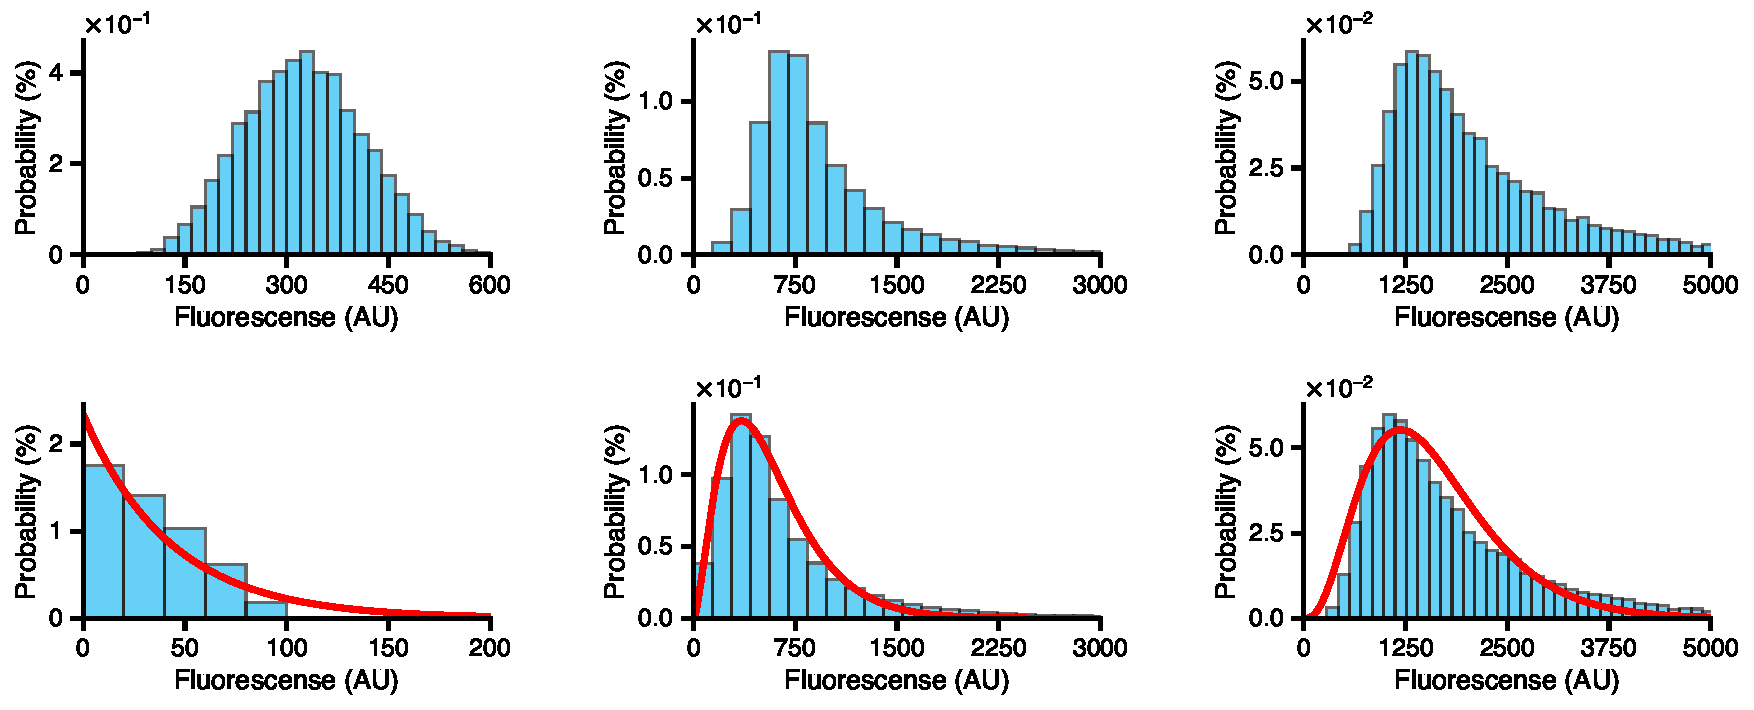
\includegraphics[width=\linewidth]{assets/addendumFig1.pdf}
    \caption{Histograms of the measured fluorescence signals (top row) and their deconvolution results (bottom row) for three RAJ11 constructs (\texttt{RAJ11M}, \texttt{RAJ11\_10}, and \texttt{RAJ11\_100}). Bars represent the empirical probability distribution of the fluorescence intensities, whereas the red curves in the bottom row denote the fitted gamma distributions based on the estimated shape and scale parameters.}\label{fig:figadd.1}
\end{figure}

We observed that the wild-type sRNA-regulated construct produces bursts of protein that lead to a heavy-tailed distribution. The deconvolved distributions represent the true protein expression variability attributable to the RAJ11 construct. All conditions yielded unimodal but highly skewed distributions of protein per cell. We observed that the wild-type sRNA-regulated construct produces bursts of protein that lead to a heavy-tailed distribution. %The fitted gamma distribution for wild-type had a moderate coefficient of variation (CV) with $\mathrm{CV}^2 \approx 0.63$ and skewness $\approx3.27$.



\begin{figure}[ht!]
    \centering
    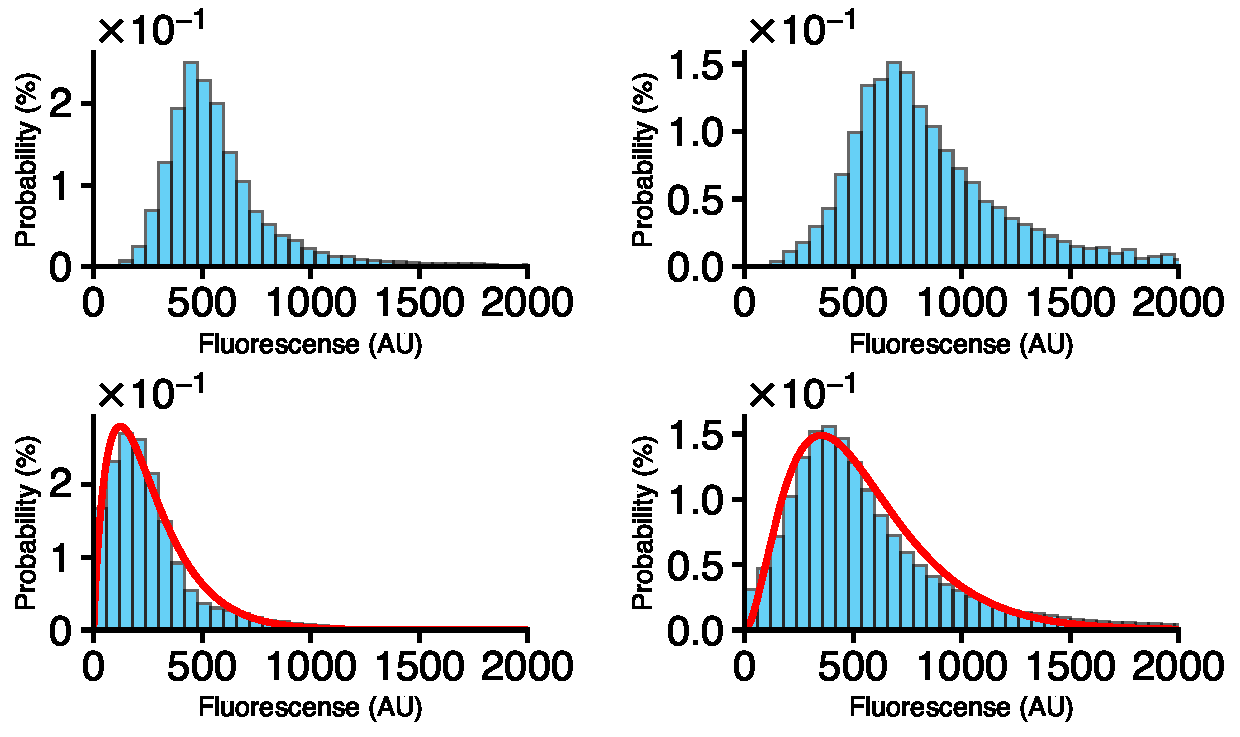
\includegraphics[width=0.67\linewidth]{assets/addendumFig2.pdf}
    \caption{Histograms of the measured fluorescence signals (top row) and their deconvolution results (bottom row) for \texttt{RAJ11\_100\_m26} (left) and \texttt{RAJ11\_100\_m32} (right). Bars depict the empirical probability distributions of the fluorescence intensities, while the red curves in the bottom panels represent fitted gamma distributions with the estimated shape and scale parameters.}\label{fig:figadd.2}
\end{figure}

%The fitted gamma distribution for wild-type had a moderate coefficient of variation (CV) with $\mathrm{CV}^2 \approx 0.63$ and skewness $\approx3.27$, indicating fluctuations somewhat lower than a Poisson process (which has $\mathrm{CV}^2=1$) despite bursty production. This suggests that frequent bursts (due to efficient sRNA binding) effectively even out protein production over time, reducing relative noise (analogous to noise buffering by microRNA regulation). In contrast, a mutant sRNA with weaker mRNA binding (RAJ11 A4T G5T) showed a more variable expression profile. Its protein distribution fit yielded $k\approx1.89$ (closer to exponential), and a nearly Poissonian noise level ($\mathrm{CV}^2\approx0.99$). The mutant's distribution maintained a similar mean fluorescence but with noticeably broader spread, consistent with more sporadic, less efficient bursting. An intermediate mutant (single base change, RAJ11 A4T) showed intermediate behavior (gamma $k\approx2.90$, $\mathrm{CV}^2\approx0.74$).

Key findings are that all sRNA-regulated cases produce right-skewed, bursty protein distributions, and weaker sRNA--mRNA interactions lead to higher noise (greater cell-to-cell variability) for a comparable mean output (\textbf{Fig. \ref{fig:figadd.1}}, \textbf{Fig. \ref{fig:figadd.2}}). These results quantitatively demonstrate post-transcriptional bursting in a real genetic system, in agreement with theoretical expectations \cite{Rodrigo2018}. Moreover, by fitting the distributions, we confirm that gamma-like forms appropriately describe the protein count variability, as seen previously in bursty gene expression systems. The wild-type sRNA effectively reduces relative noise and skewness compared to the weaker mutants, highlighting an intrinsic noise-control mechanism in the post-transcriptional bursting regime.

\section*{Discussion}
\subsection*{Mechanism of Post-Transcriptional Bursting}
Our preliminary findings suggest that that small RNAs can induce bursts of protein production by toggling translation on and off. In the RAJ11 system, the sRNA binding to the 5'UTR acts as a molecular switch: when bound, it exposes the Shine-Dalgarno sequence and triggers a period of active translation (the ``on'' state). Each binding event can generate a burst of protein until the complex dissociates or the mRNA is deactivated, at which point translation returns to ``off''. This mechanism is analogous to transcriptional bursting (where promoter states drive bursts of mRNA production) but occurs at the post-transcriptional level, downstream of mRNA synthesis. The derived burst frequency ($\sim k_{\text{on}}\langle s \rangle$) and burst size ($\sim k_p/k_{\text{off}}$) provide a useful intuitive picture: a higher sRNA concentration or binding rate increases how often bursts occur, while a slower unbinding (or inactivation) rate prolongs each translational burst, yielding more protein per burst.

Our incomplete analytical treatment (using Langevin equations and a telegraph process) is yet to reproduce these burst characteristics, consistent with previous stochastic models of gene expression bursts. Importantly, the post-transcriptional bursts we observe are a direct consequence of molecule-to-molecule variability at the RNA level (sRNA--mRNA interactions), rather than promoter state changes, which is consistent with the concept introduced by \cite{Rodrigo2018}: bursts of protein synthesis can arise ``beyond'' transcription, through dynamic RNA-level regulation.

In essence, an mRNA that is otherwise translationally silent can, upon sRNA binding, stochastically produce a flurry of protein, thereby increasing cell-to-cell heterogeneity in protein levels. Such bursts were evident in our experiments as heavy-tailed protein distributions. The right-skewed gamma distributions fitted to our data (with shape parameters $<$4) are indicative of infrequent large bursts and corroborate the idea that translational activation is episodic. These distributional signatures mirror those of classical transcriptional bursting -- for example, the negative binomial distributions reported for noisy gene expression in bacteria -- highlighting a unifying principle: bursting is a fundamental outcome of on/off dynamic regulation, whether at the promoter or post-transcriptional level.

\subsection*{Tuning of Expression Noise by sRNA--mRNA Interactions}
By comparing wild-type and mutant sRNAs, it is hinted that the kinetic parameters of sRNA binding (and unbinding) directly influence the magnitude of noise in protein expression. All variants produced similar mean protein levels in our conditions (owing to compensatory adjustments in burst frequency/duration), yet their noise profiles differed markedly. The wild-type sRNA, which has a strong binding affinity (large negative $\Delta G$ of binding), yielded a protein count distribution with lower normalized variance (CV) and moderate skewness. In contrast, the weakened-binding mutant (with seed mismatches) exhibited nearly Poisson-level noise and higher relative variance, even though the average protein output remained comparable. This trend suggests that strong sRNA binding ``smooths out'' protein production, making translation more constitutive at the single-cell level. %When binding is strong $k_\text{on}$ is high, bursts occur so frequently that they effectively overlap or the mRNA spends most of its time in the active state, leading to more steady protein accumulation (lower fractional noise).

%Conversely, when binding is weak (low $k_\text{on}$, high $k_\text{off}$), an mRNA infrequently enters the active state and for short durations, resulting in production that is bunched into rarer, brief bursts -- yielding higher cell-to-cell variability.

These observations resonate with studies of microRNA-based regulation in eukaryotes, where introducing an RNA-mediated repression can either buffer or amplify noise depending on kinetic regime \cite{Schmiedel2015}. In our bacterial case, the sRNA serves as an activator of translation, but the effect on noise is analogous: robust regulation (fast binding) buffers noise, whereas weaker regulation approaches the unregulated scenario of random translation initiation with full noise.

Notably, \cite{ArbelGoren2016} observed in an \textit{E. coli} sRNA network that noise is strongly influenced by sRNA-mediated mRNA decay and complex formation rates, which is consistent with our findings that altering sRNA--mRNA interaction strength modulates noise. Thus, our results bridge genotype (RNA sequence mutations) to phenotype (noise in protein levels): small changes in the seed region free energy (on the order of a few kcal/mol) can move the system from a relatively ``buffered'' expression regime to a highly stochastic one, without significantly changing mean expression. This tunability is of great interest for synthetic biology, as it offers a knob to adjust phenotypic variability independently of mean output \cite{Levine2007, Mutalik2012}.

Moreover, the ability to tune noise via RNA regulators supports the idea that cells could evolve or select for different noise levels by mutations in non-coding regions -- adding an evolutionary dimension to the role of post-transcriptional regulation.

\subsection*{Comparison to Transcriptional Bursting and Biological Implications}
It is insightful to compare the bursting we observe post-transcriptionally with the well-characterized phenomenon of transcriptional bursting. Transcriptional bursts (arising from promoters switching between inactive and active states) also produce heavy-tailed mRNA distributions and super-Poissonian noise \cite{Ozbudak2002}. In our post-transcriptional bursting, the ultimate protein distributions can be mathematically similar (e.g. both can often be described by negative binomial statistics), but the mechanistic origin is different: instead of promoter chromatin or transcription factor binding kinetics, it is the RNA-RNA interaction kinetics that set the burst parameters. One practical implication is in the timing and integration of cellular decisions. Transcriptional bursting is often implicated in fate determination events by providing occasional high transcript pulses. Post-transcriptional bursting could likewise generate heterogeneity in protein levels from uniformly transcribed mRNAs, thereby enabling phenotypic diversification without changes at the DNA level. This may be particularly relevant in stress responses or developmental contexts where small RNAs are known to play critical regulatory roles. Our results underscore that the RNA layer adds an additional opportunity for noise modulation in gene expression.

The distinctive feature of post-transcriptional bursts is that they can be rapidly tunable by introducing or modulating a regulatory RNA. In contrast, altering transcriptional burst kinetics often requires promoter mutations or changing transcription factor dynamics. From an evolutionary perspective, an organism might employ sRNA regulators to finetune expression noise on short evolutionary timescales (since RNA sequences can mutate to adjust binding affinity) while keeping the mean expression of a gene constant. This could be advantageous for bet-hedging strategies in fluctuating environments, or for coordinating multi-gene networks where only certain genes' expression noise needs adjustment. In summary, our study demonstrates that post-transcriptional bursting is a distinct but analogous phenomenon to transcriptional bursting, broadening the paradigm of how stochastic gene expression can arise. It highlights the often under-appreciated role of RNA interactions in generating phenotypic diversity, supporting the view that gene regulation at the RNA level is as significant as DNA-level regulation in shaping cellular heterogeneity.

Future investigations could explore the interplay of transcriptional and post-transcriptional bursts occurring together, and how cells orchestrate these layers of regulation to achieve desired expression dynamics \cite{Tanenbaum2014}. Our findings not only contribute to the fundamental understanding of gene expression noise but also provide design principles for constructing synthetic gene circuits with controllable noise via sRNA regulators.

\section*{Materials and Methods}
\subsection*{RAJ11 Construction Configuration}
The wild-type RAJ11 configuration deesigned on \cite{Rodrigo2015} comprises two core genetic elements: an sRNA module specifically designed to bind a complementary stretch of nucleotides (the ``toehold'') on the 5' UTR of the target mRNA, and a 5' UTR whose native secondary structure sequesters the ribosome-binding site (RBS). In the absence of the sRNA, this 5' UTR hairpin prevents ribosomes from accessing the RBS, resulting in minimal basal translation. The sRNA was computationally optimized in \cite{Rodrigo2015} to expose a highly accessible seed region that can quickly and stably hybridize to the 5' UTR. Once bound, the intramolecular hairpin in the mRNA is destabilized, making the RBS accessible for translation initiation. This design achieves tight cis-repression of the downstream GFP gene, followed by robust trans-activation only when the RAJ11 sRNA is present.

In addition to the wild-type RAJ11 configuration (referred to here as \texttt{RAJ11M}), we generated two key mutants, \texttt{RAJ11\_m26} and \texttt{RAJ11\_m32}, each introducing specific nucleotide substitutions that either modify the seed region of the sRNA or its complementary segment on the 5' UTR. For instance, \texttt{RAJ11\_m26} carries selected base changes in the sRNA seed to evaluate how disruptions in base-pair complementarity affect binding kinetics, whereas \texttt{RAJ11\_m32} alters nucleotides within the 5' UTR to test changes in RBS accessibility under partial or complete mismatch scenarios. By comparing the dynamic range of GFP expression across these constructs, we aimed to determine the extent to which each mutation weakens sRNA--mRNA pairing. This systematic set of mutants was instrumental for validating our thermodynamic predictions step by step, as it allowed us to link specific sequence changes to measurable shifts in translational activation.

Furthermore, we placed the \texttt{RAJ11M} configuration in both a high-copy-number plasmid (\texttt{RAJ11M}) and a low-copy-number plasmid (\texttt{RAJ11M\_P15}), and tested each under varying levels of anhydrotetracycline (ATC) induction, specifically 0 ng/mL (\texttt{RAJ11M}), 10 ng/mL (\texttt{RAJ11\_10}), and 100 ng/mL (\texttt{RAJ11\_100}). We then introduced the \texttt{RAJ11\_m26} and \texttt{RAJ11\_m32} mutants with 100 ng/mL of ATC (\texttt{RAJ11\_100\_m26} and \texttt{RAJ11\_100\_m32}). By comparing the resulting GFP outputs across these plasmid backgrounds and induction levels, we aimed to evaluate how increased sRNA transcription affects riboregulation in both wild-type and mutant variants.

\subsection*{Mathematical Model of sRNA-Mediated Gene Expression} We adopted the stochastic modeling framework described in \cite{Rodrigo2018} to describe a gene post-transcriptionally regulated by a small RNA. The system consists of an mRNA ($x$) and its protein product ($y$). Transcription of mRNA occurs with rate $k_m$, $c$ is the copy number of the gene, and translation of protein occurs only when the mRNA is in an active state (ribosome-binding site accessible) with rate $k_p$. The sRNA binding toggles this state. We formalized this using two coupled Langevin equations (Ito stochastic differential equations) for $x(t)$ and $y(t)$:

\begin{equation} \frac{dx}{dt} = c k_m - \gamma_m x + \sqrt{c k_m + \gamma_m x}\xi_m(t) \end{equation}

\begin{equation} \frac{dy}{dt} = k_p\zeta(t) - \gamma_p y + \sqrt{k_p,\zeta(t) + \gamma_p y}\xi_p(t) \end{equation}

where $\gamma_m$ and $\gamma_p$ are the degradation rates of mRNA and protein, respectively (so $1/\gamma_m$, $1/\gamma_p$ are their average lifetimes). The terms $\xi_m(t)$ and $\xi_p(t)$ represent independent Gaussian white noise processes (with $\langle \xi_i(t)\rangle=0$ and $\langle \xi_i(t)\xi_j(t')\rangle=\delta_{ij}\delta(t-t')$) accounting for intrinsic stochastic fluctuations.

The steady state solution for $\mathbb{E}[x(t)]$ is given by

\begin{align*}
    0 &= \mathbb{E}\left[c k_m - \gamma_m x + \sqrt{c k_m + \gamma_m x}\xi_m(t)\right]\\
    0 &= c k_m - \gamma_m \mathbb{E}[x]\\
    \mathbb{E}[x(t)] &= \frac{c k_m}{\gamma_m}
\end{align*}

We can only get this expression through 3 important assumptions:

\begin{enumerate} \item The noise term is zero on average (given by the white noise process). \item The amplitude of the stochastic process and the stochastic process are uncorrelated, hence the expectation of the product is the product of the expectations. \item We are using the mean-field approximation, i.e. the amplitude of the noise is finite, hence it disappears when multiplying by 0. \end{enumerate} Now that we have the expression for $\left\langle x\right\rangle$, we can substitute it back into the original equation by means of the mean-field approximation ($x = \left\langle x\right\rangle + \Delta x$):

\begin{align*}
    \frac{d\left(\mathbb{E}[x] + \Delta x(t)\right)}{dt} &= c k_m - \gamma_m\left(\mathbb{E}[x] + \Delta x(t)\right) + \sqrt{c k_m + \gamma_m\left(\mathbb{E}[x] + \Delta x(t)\right)}\xi_m(t)\\
    \frac{d\Delta x(t)}{dt} &= c k_m - \gamma_m\mathbb{E}[x] - \gamma_m\Delta x(t) + \sqrt{c k_m + \gamma_m\mathbb{E}[x]}\xi_m(t)\\
    \frac{d\Delta x(t)}{dt} &= -\gamma_m\Delta x(t) + \sqrt{2c k_m}\xi_m(t)
\end{align*}

To solve the above equation, we will use the Fourier transform of the equation. We'll denote the Fourier transform of $f$ as $\hat{f}$, equivalently as $\mathcal{F}\left\{f\right\}$. In this analysis, we assume that $\Delta x(t)$ is interpreted within the framework of tempered distributions, specifically belonging to the dual space $\mathcal{S}'(\mathbb{R})$ of the Schwartz space. This assumption guarantees that the Fourier transform is well-defined, even though white noise is not square-integrable in the classical sense.

\begin{align*}
    \mathcal{F}\left\{\frac{d\Delta x(t)}{dt}\right\} &= \mathcal{F}\left\{-\gamma_m\Delta x(t) + \sqrt{2ck_m}\xi_m(t)\right\}\\
    i\omega\hat{\Delta x}(\omega) - \Delta x_0&= -\gamma_m\hat{\Delta x}(\omega) + \sqrt{2ck_m}\hat{\xi}_m(\omega)\\
    \hat{\Delta x}(\omega) &= \left(\frac{\sqrt{2ck_m}}{i\omega + \gamma_m}\right)\hat{\xi}_m(\omega)
\end{align*}

This shows that the transfer function from noise to mRNA fluctuations is given by $G_x(i\omega) = \frac{\sqrt{2 c k_m}}{\gamma_m + i\omega}$. Note that we have proceeded with the assumption that the initial condition is zero ($\Delta x_0 = 0$). The next step of the derivation involves using the convolution theorem.

\begin{untheorem}[Convolution theorem]
    Let $f$ and $g$ be two functions with Fourier transforms $\hat{f}$ and $\hat{g}$, respectively. Then the convolution of $f$ and $g$, denoted as $f*g$ is given by:
    \begin{equation*}
        f(t)*g(t) = \mathcal{F}^{-1}\left\{\hat{f}(\omega)\hat{g}(\omega)\right\}
    \end{equation*}
\end{untheorem}

In simpler terms, the Fourier transform of the convolution of two functions equals the product of the Fourier transforms of each of the functions. In our particular case, we have 

\begin{equation*}
    \hat{\Delta x(\omega)} = \hat{g}(\omega)\hat{\xi}_m(\omega)
\end{equation*}

where $\hat{g}(\omega) = \left(\frac{\sqrt{2ck_m}}{i\omega + \gamma_m}\right)$. Therefore,

\begin{equation*}
    \Delta x(t) = \int_0^t\xi_m(\tau)g(t-\tau)d\tau
\end{equation*}

It is then necessary to compute the inverse Fourier transform of $\hat{g}(\omega)$. Our primary objectives are to verify the convergence of the integral obtained via the inverse Fourier transform and to explicitly address the behavior for $t<0$. In this context, we note that for $t<0$ the solution is defined to be zero, corresponding to the general form $H(t)e^{-\alpha t}$, where $H(t)$ is the Heaviside step function. Since the convolution integral is evaluated over the interval $(0,t)$, the case for $t<0$ is naturally excluded. The inverse Fourier transform of $\hat{g}(\omega)$ is given by:

\begin{align*}
g(t) &= \mathcal{F}^{-1}\left\{\hat{g}(\omega)\right\}\\
&= \left(\sqrt{2ck_m}\right)\mathcal{F}^{-1}\left\{\frac{1}{i\omega+\gamma_m}\right\}\\ 
&= \left(\sqrt{2ck_m}\right)\frac{1}{2\pi}\int_{-\infty}^{+\infty}\frac{1}{i\omega+\gamma_m}e^{i\omega t}d\omega
\end{align*}

Let's define $g(z) = \frac{1}{iz+\gamma_m}$, with $z\in\mathbb{C}$. We will introduce the following theorems:

\begin{untheorem}
    Suppose $f(z)$ is a function of $z\in\mathbb{C}$ and $f(z)$ is defined in the upper-half plane. If there is an $a>1$ and $M>0$ such that

    $$
    \left|f(z)\right| < \frac{M}{\left|z\right|^a}
    $$
  
    for a large $\left|z\right|$, then 
  
    $$
    \lim_{R\to\infty}\int_{C_R}f(z)dz = 0
    $$
  
    Where $C_R$ is the path (in this case an arch) that goes from $R$ in the real axis and goes back to $-R$ through the upper-half plane. This theorem is for functions that decay faster than $\frac{1}{z}$.
\end{untheorem}

\begin{untheorem}\label{theorem:complex_square}
    Suppose $f(z)$ is a function of $z\in\mathbb{C}$ and $f(z)$ is defined in the upper-half plane. If there is $M>0$ such that

    $$
    \left|f(z)\right| < \frac{M}{\left|z\right|}
    $$
  
    for a large $\left|z\right|$, then 
  
    $$
    \lim_{x_1\to\infty,x_2\to\infty}\int_{C_1+C_2+C_3}f(z)e^{iaz}dz = 0
    $$
  
    Where $C_1+C_2+C_3$ is a rectangular path that goes from point $x_1$ in the real axis up to the upper-half plane until height $(x_1+x_2)i$, then goes to the left until $-x_2$ and goes down to the real axis. This theorem is for functions that decay like $\frac{1}{z}$.
\end{untheorem}

For our particular case, we'll use the previous theorem (as we can see that $g(z)$ decays like $\frac{1}{z}$). So, we need to find a value of $M>0$ so that the bound holds:

\begin{align*}
\left|g(z)\right| &= \left|\frac{1}{iz+\gamma_m}\right|\\
&= \frac{1}{\left|iz+\gamma_m\right|}\\
&= \frac{1}{\sqrt{(\text{Re}(z))^2 + (\gamma_m - \text{Im}(z))^2}}\\
&= \frac{1}{\sqrt{\gamma_m^2 - 2\gamma_m\text{Im}(z) + \text{Re}^2(z) +\text{Im}^2(z)}}\\
&= \frac{1}{\sqrt{\gamma_m^2 - 2\gamma_m\text{Im}(z) + \left|z\right|^2}}\\
\end{align*}

for a large $\left|z\right|$, we can see that $\left|g(z)\right| \approx \frac{1}{\left|z\right|}$, so we can use the theorem as any $M>1$ is sufficient to make the bound hold:

\begin{align*}
\left|g(z)\right| &= \frac{1}{\sqrt{\gamma_m^2 - 2\gamma_m\text{Im}(z) + \left|z\right|^2}}\\
&\approx \frac{1}{\left|z\right|} < \frac{M}{\left|z\right|}\\
\end{align*}

With this condition met, we can use the standard contour $C_1+C_2+C_3 + C_4$ which forms a rectangle that goes from point $x_1$ in the real axis up to the upper-half plane until height $(x_1+x_2)i$, then goes to the left until $-x_2$, then goes down to the real axis and finally goes back to our starting point. Note then that if we take the limits $x_1\to\infty$ and $x_2\to\infty$ on contour $C_4$, we have our original integral (the one from the inverse Fourier transform):

$$
\lim_{x_1\to\infty, x_2\to\infty}\int_{C_4}g(z)e^{iaz}dz = \lim_{x_1\to\infty, x_2\to\infty}\int_{-x_2}^{x^1}\frac{e^{iz t}}{iz+\gamma_m}dz
$$

Furthermore, given the bound $M > 1$ we know that

$$
\lim_{x_1\to\infty, x_2\to\infty}\int_{C_1+C_2+C_3}g(z)e^{iaz}dz = 0
$$

Therefore, the entire contour integral over $C_1 + C_2 + C_3 + C_4$:

\begin{align*}
\lim_{x_1\to\infty, x_2\to\infty}\int_{C_1+C_2+C_3+C_4}g(z)e^{iaz}dz &= 0 + \lim_{x_1\to\infty, x_2\to\infty}\int_{C_4}\frac{e^{izt}}{iz+\gamma_m}dz
\end{align*}

So, the inverse Fourier transform is given by the contour integral over $C_1 + C_2 + C_3 + C_4$. We can then use the residue theorem to compute the integral.

\begin{untheorem}[Cauchy's Residue Theorem]
    Let $f(z)$ be a function that is analytic in a region $D$ except for a finite number of isolated singularities. For any simple closed curve $C$ that is positively oriented and lies in $D$:
    $$
    \oint_C f(z)dz = 2\pi i\sum_{k=1}^{n} \text{Res}(f,z_k)
    $$
    where $z_k$ are the singularities of $f(z)$ in $D$ and $\text{Res}(f,z_k)$ denotes the residue of $f$ at $z_k$.
\end{untheorem}

The residue of a function $f(z)$ at a point $z_0$ is given by:

$$
\text{Res}(f,z_0) = \lim_{z\to z_0} (z-z_0)f(z)
$$

In our case, we have a simple pole at $z = \gamma_m i$, as the denominator of $g(z)$ is zero at $z = \gamma_m i$. Since $\gamma_m > 0$, we have that the pole is in the upper-half plane. In addition, the pole is a simple pole, we can compute the residue through the definition:

\begin{align*}
\text{Res}(g,\gamma_m i) &= \lim_{z\to \gamma_m i} (z-\gamma_m i)\left(\frac{e^{izt}}{iz+\gamma_m}\right)\\
&= e^{-\gamma_mt}\lim_{z\to \gamma_m i} \left(\frac{z-\gamma_m i}{iz+\gamma_m}\right)\\
&= \frac{e^{-\gamma_mt}}{i}\lim_{z\to \gamma_m i} \left(\frac{iz +\gamma_m}{iz+\gamma_m}\right) = \frac{e^{-\gamma_mt}}{i} = -ie^{-\gamma_mt}\\
\end{align*}

Now we can use Cauchy's Residue Theorem to compute the integral:

\begin{align*}
\int_{C_4}\frac{e^{iz t}}{iz+\gamma_m}dz &= 2\pi i\text{Res}(g,\gamma_m i)\\
&= 2\pi i\left(-ie^{-\gamma_mt}\right)\\
&= 2\pi e^{-\gamma_mt}
\end{align*}

Returning to the inverse Fourier transform, we have:

\begin{align*}
g(t) &= \left(\sqrt{2ck_m}\right)\left(\frac{1}{2\pi}\int_{-\infty}^{\infty}\frac{e^{i\omega t}}{i\omega+\gamma_m}d\omega\right)\\
&= \sqrt{2ck_m}e^{-\gamma_mt}
\end{align*}


Therefore, the general solution for $\Delta x(t)$ is given by:

\begin{align*}
\Delta x(t) &= \int_0^t \xi_m(\tau)g(t-\tau)d\tau\\
&= \sqrt{2ck_m}\int_0^t \xi_m(\tau)e^{-\gamma_m(t-\tau)}d\tau
\end{align*}

Besides the above, we can also compute the spectral density of $\Delta x(t)$, which we'll denote as $S_{\Delta x}$. The spectral density is defined as the squared absolute value of the Fourier transform of the process. So for our process, we have that

\begin{align*}
S_{\Delta x} &= \left|\mathcal{F}\left\{\Delta x\right\}\right| = \left|\hat{\Delta x}\right|^2\\
&= \left|\sqrt{2ck_m}\left(\frac{1}{i\omega+\gamma_m}\right)\hat{\xi}_m(\omega)\right|^2\\
&= \left(\frac{2ck_m}{\omega^2+\gamma_m^2}\right)\left|\hat{\xi}_m(\omega)\right|^2\\
\end{align*}

Do note that one needs to be extra careful when using these definitions, because the Fourier transform of white noise process is defined only as a kind of limit of smooth processes. Fortunately, as long as we only work with linear systems this definition indeed works. And it provides a useful tool for determining covariance functions of stochastic differential equations.

A great property is that, since the Fourier transform of white noise is a constant (imagine a white noise signal in the time domain; it appears as a random fluctuation where the amplitude changes rapidly and unpredictably. When the Fourier transform of this signal is taken to analyze its frequency components, it can be seen that there is no preference for any specific frequency; all frequencies are equally likely to contribute to the noise), the spectral density of the process is also a constant.

Therefore

\begin{align*}
S_{\Delta x} &= \left(\frac{2ck_m}{\omega^2+\gamma_m^2}\right)\left|\hat{\xi}_m(\omega)\right|^2\\
&= \frac{2ck_m}{\omega^2+\gamma_m^2}\\
\end{align*}


Next we need to introduce the Wiener-Khinchin theorem.

\begin{untheorem}[Wiener-Khinchin]
    For a wide-sense stationary random process, the power spectral density $S_x(\omega)$ and the autocorrelation function $C_x(t)$ form a Fourier transform pair:
    $$
    S_x(\omega) = \mathcal{F}\{C_x(t)\} \quad \text{and} \quad C_x(t) = \mathcal{F}^{-1}\{S_x(\omega)\}
    $$
    where $\mathcal{F}$ denotes the Fourier transform and $\mathcal{F}^{-1}$ its inverse.
\end{untheorem}

Let's denote the autocorrelation function of $\Delta x(t)$ as $C_{\Delta x}$, so by means of the Wiener-Khinchin theorem, we have that

\begin{align*}
C_{\Delta x} &= \mathcal{F}^{-1}\left\{S_{\Delta x}\right\}\\
&= \mathcal{F}^{-1}\left\{\frac{2ck_m}{\omega^2+\gamma_m^2}\right\}\\
&= \frac{2ck_m}{2\gamma_m}\mathcal{F}^{-1}\left\{\frac{2\gamma_m}{\omega^2+\gamma_m^2}\right\}\\
&= \frac{ck_m}{\gamma_m}e^{-\gamma\left\lvert \Delta t\right\rvert}
\end{align*}

Note that the inverse Fourier transform here was computed using the property of the Fourier transform being a linear operator, and using the known result that $\mathcal{F}^{-1}\left\{\frac{2\alpha}{\alpha^2 + \omega^2}\right\} = e^{\alpha\left\lvert t\right\rvert}$

With these definitions, it is left to compute the statistical properties of the protein $y(t)$, which is left unsolved as this work is yet to be published.

% The key state variable $\zeta(t)$ is a two-state (0/1) telegraph process representing whether an mRNA is translationally active at time $t$. Specifically, $\zeta=0$ corresponds to the mRNA's ribosome-binding site being occluded (translation ``off''), and $\zeta=1$ corresponds to the mRNA being bound by sRNA in such a way that the ribosome-binding site is exposed (translation ``on''). The switching of $\zeta$ is governed by the sRNA--mRNA interaction kinetics.: we denote $k_{\text{on}}$ as the rate at which an inactive mRNA becomes active (sRNA binding or action) and $k_{\text{off}}$ as the rate at which an active mRNA returns to inactive (sRNA unbinding or complex inactivation). In steady state, $\zeta(t)$ has an average value equal to the fraction of time an mRNA is in the on state. We define $p_{\text{on}} = \frac{k_{\text{on}}\langle s\rangle}{k_{\text{on}}\langle s\rangle + k_{\text{off}}}$ as the equilibrium probability an mRNA is active (here $\langle s\rangle$ is the average free sRNA concentration). The autocorrelation of the telegraph process decays with a characteristic time $\tau \approx (k_{\text{on}}\langle s\rangle + k_{\text{off}})^{-1}$, and for an ideal telegraph one has $\langle \zeta(t)\zeta(0)\rangle - \langle \zeta \rangle^2 \propto e^{-t/\tau}$. In our model, we set $\langle \zeta(t)\rangle = \langle x \rangle p_{\text{on}}$ to reflect that the number of active mRNAs is bounded by total mRNAs.

% We note that this formulation effectively assumes the sRNA is present and dynamically binding; in the absence of sRNA, $p_{\text{on}}\to0$ and translation events are negligible. To analyze the model, we first solved for the steady-state mean mRNA. Setting $d\langle x\rangle/dt=0$ in the mRNA equation and using $\langle \xi_m(t)\rangle=0$, we obtain $0 = c k_m - \gamma_m \langle x\rangle$, hence $\langle x\rangle = c k_m/\gamma_m$. This result relies on the mean-field approximation that $\langle \sqrt{\gamma_m x},\xi_m\rangle = 0$ (justified by the noise being zero-mean and uncorrelated with amplitude to first order). We then performed a fluctuation analysis by writing $x(t) = \langle x\rangle + \Delta x(t)$ and linearizing. This yields an Ornstein--Uhlenbeck type equation for the mRNA fluctuations:

% \begin{equation}
%     d(\Delta x)/dt \approx -\gamma_m \Delta x + \sqrt{2c k_m},\xi_m(t)    
% \end{equation}

% after substituting $\langle x\rangle$ into the noise term. The solution of this linear stochastic differential equation was obtained via Fourier transform methods. In the frequency domain, the transfer function from noise $\xi_m$ to mRNA output $\Delta x$ is $G_x(i\omega) = \frac{\sqrt{2 c k_m}}{\gamma_m + i\omega}$. From this, we computed the mRNA power spectral density and autocorrelation, confirming that mRNA fluctuations follow an exponential relaxation with correlation time $1/\gamma_m$ (consistent with a simple birth--death process). These analytical results (notably, that the Fano factor of mRNA is 1 at steady state, as expected for a Poissonian transcript process) provided a baseline for understanding how translational bursting influences the protein statistics. For the protein $y(t)$, the production term is modulated by $\zeta(t)$. Rather than deriving an explicit analytical solution for $y(t)$ (which leads to a system of integro-differential equations due to the two-state switching), we utilized stochastic simulation to capture the protein burst statistics. We implemented Gillespie's exact stochastic simulation algorithm (SSA) \cite{Gillespie2007} to generate trajectories of the coupled $(x,\zeta,y)$ system. In the SSA, transcription, translation (when $\zeta=1$), switching on, and switching off are treated as reaction channels with propensities $c k_m$, $k_p x$ (active only if $\zeta=1$), $k_{\text{on}} s x$ (sRNA binds an available mRNA; we update $s$ accordingly if tracking sRNA pool), and $k_{\text{off}} x_{\text{active}}$ (active mRNA switches off) respectively. Each simulation step advances the system by sampling the next reaction and time increment from exponential waiting-time distributions.

% Parameter values were chosen in line with prior experimental and modeling studies of bacterial gene expression. We used $c=1$ (single-copy gene). The transcription rate $k_m$ and decay rate $\gamma_m$ were set such that $\langle x \rangle$ is on the order of 1--10 mRNAs per cell (a few transcripts per cell, typical for low-expression genes). The translation rate $k_p$ and protein decay (dilution) rate $\gamma_p$ were set to yield mean protein levels in the range of tens to a few hundred per cell (matching the scale of our fluorescence measurements). For instance, in dimensionless units, we often took $\gamma_m=1$,min$^{-1}$, $k_m=1$,min$^{-1}$ (so $\langle x\rangle=1$ mRNA), $k_p=20$,min$^{-1}$, and $\gamma_p=0.05$,min$^{-1}$ (protein half-life on the order of hours), although for the RAJ11 constructs the effective protein degradation includes dilution in dividing \textit{E. coli}, so $\gamma_p \sim 0.02$--0.03,min$^{-1}$. The on/off switching rates were inferred from thermodynamic calculations (see below) but tested in simulations over a range consistent with those free energies. We simulated long enough to collect stable protein distributions (typically $>10^4$ minutes, discarding transients).

% \subsection*{Thermodynamic Analysis of sRNA--mRNA Interactions}

% To parameterize $k_{\text{on}}$ and $k_{\text{off}}$ for the RAJ11 sRNA--mRNA pair and its mutants, we performed RNA secondary structure and free energy calculations. We used NUPACK (v4) to compute the minimum free energy (MFE) structures for: (i) the 5'UTR of the mRNA alone (cis-RAJ11), (ii) the sRNA alone (trans-RAJ11), and (iii) the sRNA--mRNA duplex (co-folded complex). The wild-type sequences and two mutant sRNA sequences (with seed region mutations A4U and G5U, individually and combined) were analyzed. The MFE of the mRNA alone ($\Delta G_m$) was found to be -14.4 kcal/mol, corresponding to a hairpin that sequesters the ribosome binding site (SD sequence). The sRNA alone has a stable structure ($\Delta G_s \approx -37.1$ kcal/mol).

% For the sRNA--mRNA complex, we obtained an overall free energy $\Delta G$ (duplex formation) and an activation free energy $\Delta G^\ddagger$ associated with initiating the interaction \cite{Rodrigo2015}. For wild-type RAJ11, the duplex MFE was $\Delta G \approx -14.5$ kcal/mol, roughly equal (in magnitude) to the mRNA hairpin energy, implying the complex formation just compensates the cost of opening the mRNA hairpin. The reported $\Delta G^\ddagger$ for this interaction was about -10.3 kcal/mol. For the single-mutant sRNA (A4U), the duplex MFE was weaker ($\Delta G \approx -10.1$ kcal/mol) and the effective $\Delta G^\ddagger \approx -5.9$ kcal/mol. The double-mutant (A4U G5U) showed a substantially reduced binding stability: $\Delta G \approx -6.5$ kcal/mol and $\Delta G^\ddagger \approx -3.7$ kcal/mol. These thermodynamic parameters indicate that the mutant sRNAs have lower affinity for the target mRNA and likely slower binding kinetics. We leveraged these values to estimate the kinetic rates using an Arrhenius/Kramers approach \cite{Hanggi1990}. In this scheme, we set:

% \begin{equation}
%     k_{\text{on}} = A \exp(-\Delta G^\ddagger/RT) 
% \end{equation}

% \begin{equation}
%     k_{\text{off}} = A \exp(-(\Delta G^\ddagger - \Delta G)/RT)
% \end{equation}

% where $A$ is a frequency factor (related to diffusion-limited collision frequency, set on the order of $10^6$--$10^7$ M$^{-1}$s$^{-1}$ for RNA interactions in the cell) and $RT$ is the thermal energy (we assume $T=310$ K, so $RT\approx0.616$ kcal/mol). This nonequilibrium two-state model ensures that the ratio $k_{\text{on}}/k_{\text{off}} = \exp(-\Delta G/RT)$, matching the equilibrium binding constant from the free energy of duplex formation. We used the above relations to compute baseline $k_{\text{on}}$ and $k_{\text{off}}$ for simulations: for wild-type, $\Delta G^\ddagger - \Delta G \approx 4.2$ kcal/mol, so if we assume a modest $A$ (yielding $k_{\text{on}}$ on the order of $0.1$ min$^{-1}$), we get $k_{\text{off}}$ roughly one order of magnitude smaller (favoring the on-state). For the weakest mutant, $\Delta G^\ddagger - \Delta G \approx 3.7 - (-6.5) = 10.2$ kcal/mol (if interpreted directly, but note $\Delta G^\ddagger$ was given negative; in practice the barrier for binding is much higher relative to the net gain), leading to a much larger $k_{\text{off}}/k_{\text{on}}$ ratio. In qualitative terms, wild-type is expected to spend most time in the active state (high $p_{\text{on}}$), whereas the mutant might have $p_{\text{on}} \ll 1$ under similar sRNA concentrations. These rates were fed into the SSA simulations and also used in theoretical calculations of expected burst statistics.

\subsection*{Data Collection and Analysis}
For experimental validation, \textit{E. coli} cells carrying the RAJ11 construct were analyzed by flow cytometry. The construct consisted of a reporter gene with the cis-RAJ11 5'UTR and a constitutive promoter, and sRNA (trans-RAJ11) expressed from a regulated promoter. We collected single-cell fluorescence distributions for: (1) no sRNA (sRNA promoter off), (2) wild-type sRNA (induced to a certain level, labeled ``100'' which corresponds to a saturating inducer concentration), and (3) two sRNA mutants (with the same induction level). Three biological replicate samples were measured for each condition. To isolate the true protein signal distribution, we performed a deconvolution to subtract autofluorescence. The autofluorescence (background fluorescence of cells with no reporter) was measured and its distribution $b(x)$ obtained as a histogram. The raw fluorescence distribution with the reporter (which includes both background and reporter signal) is denoted $a(x)$. We treated the relationship as a convolution $a(x) = (b * c)(x)$, where $c(x)$ is the sought distribution of true reporter signal.

We implemented the deconvolution in Python by constructing the convolution matrix $B$ for $b$ and solving the linear system $B,\hat{c} = a$ for $\hat{c}$ (discrete approximation of the convolution equation). Because this inverse problem is ill-posed and $B$ is non-square, we obtained a least-squares solution with Tikhonov regularization (ridge regression) to enforce smoothness and non-negativity. Specifically, we solved $(B^T B + \lambda I)\hat{c} = B^T a$ with regularization parameter $\lambda=1$ (chosen empirically to suppress high-frequency noise in $\hat{c}$ without over-smoothing). The solution $\hat{c}(x)$ was taken as the deconvolved probability density of cellular fluorescence due to the reporter. We validated the deconvolution by reconvolving $\hat{c}$ with $b$ to obtain $\hat{a}$ and comparing it to the measured $a$. The coefficient of determination $R^2$ between $a$ and $\hat{a}$ was above 0.95 in all cases, indicating a good fit. We also computed a $t$-statistic to confirm that $\hat{c}$ significantly improved the fit over a null model. 

The deconvolved distributions $\hat{c}(x)$ for each condition were then analyzed to extract quantitative descriptors of bursting. We fit each distribution with a gamma distribution, $P(x) = x^{k-1}e^{-x/\theta}/[\Gamma(k)\theta^k]$, using maximum likelihood (via SciPy's \texttt{fit} function). This provided the shape parameter $k$ and scale $\theta$ for each condition, along with estimates of uncertainty. The fits were visually excellent and yielded $R^2>0.95$ in each case. From the theoretical distribution and from the raw data, we calculated the mean, variance, noise (defined as variance divided by mean squared, $\mathrm{CV}^2$), and skewness for each condition. These higher moments characterize bursty distributions: a Poisson distribution has $\mathrm{CV}^2=1$ and skewness = 1 (if treated as counts); higher values indicate more burstiness/variability. We found skewness strictly higher than 1 for all cases, indicating that the distributions are indeed bursty. Nonetheless, further analysis of the data is needed to confirm the validity of the theoretical model.

% The wild-type sRNA condition showed the lowest noise and a higher effective burst size (since its gamma shape $k$ was highest), whereas the mutant with two seed mismatches showed nearly Poisson noise (indicating bursts are minimal, translation events largely independent). These metrics were consistent with the qualitative behavior observed in simulations. All analyses were conducted in Python 3.8 using numpy, pandas, and SciPy; plots were generated with matplotlib. Where appropriate, we cross-validated the simulation results with the analytical model (e.g., ensuring the mean expressions and trends in noise vs. binding strength matched predictions). We also compared our results with prior literature to ensure our definitions of noise and burst statistics were standard. The combination of theoretical modeling, simulation, and experimental distribution deconvolution allowed us to rigorously characterize post-transcriptional bursting in the RAJ11 system.
\vfill
\section*{Conclusions}
This work takes a glipse into the pivotal role of sRNA-induced post-transcriptional regulation in shaping gene expression variability, looking to complement the well-characterized phenomenon of transcriptional bursting. Drawing on our modeling framework, single-cell fluorescence data, and the systematic exploration of wild-type vs. mutant sRNA constructs, we seek to demonstrate that sRNA-mediated translational on/off switching can yield robust bursts of protein production and generate heavy-tailed protein distributions. We envision these results to add depth to our understanding of multiscale biological noise: while transcriptional events can encode bursts at the mRNA level, the additional sRNA layer provides another point at which stochastic fluctuations may be amplified, modulated, or buffered. 

These fluctuations, in turn, do contribute to a hierarchical cascade of noise propagation, where molecular-level stochasticity accumulates and integrates across multiple regulatory layers to ultimately shape macroscopic phenotypic variation. This multi-level aggregation of noise sources parallels other biological phenomena where microscopic randomness gives rise to emergent stochastic behaviors at larger scales -- from protein conformational dynamics to evolutionary trajectories. Indeed, just as the superposition of multiple noise sources in gene expression can lead to non-Poissonian statistics and complex temporal patterns, the integration of various molecular-level mutational processes across different genes can collectively drive anomalous diffusion-like behaviors in evolutionary dynamics. Understanding these connections between microscopic stochasticity and macroscopic phenomenology is crucial for developing accurate quantitative models of biological variation across scales, and is yet to be fully uncovered.

\vfill

\pagebreak

\bibliographystyle{assets/rodrigostyle}
\bibliography{references/addendumReferences}

\vfill
\pagebreak ~

% General discussion
\chapter{General Discussion}

\begin{flushright}
    \textit{People think that mathematics is complicated.\\Mathematics is the simple bit, it's the stuff we can understand.\\It's cats that are complicated.}\\
    --- John H. Conway
\end{flushright}

\vspace{1cm}

This work set out to examine how stochastic dynamics shape both viral genome evolution and post-transcriptional regulatory programs. By uniting large-scale sequence analysis with mechanistic modeling, it challenged long-held assumptions of constant molecular clocks and purely transcription-focused gene regulatory frameworks. We explored RNA virus genomes as prime examples of dynamic molecular automata, investigating how mutations accumulate over time and whether these changes align with the classic neutral theory \cite{kimura1968,Zuckerkandl1965}. In addition, we briefly explored how bursty translational regulation as a source of noise that can create distinct gene expression states using synthetic gene circuits in bacteria as case study \cite{Elowitz2002,Dolcemascolo2022}. Together, these projects advanced a core hypothesis: biological systems often deviate from simple, uniform models, and statistical-based methods are essential for fully understanding their complexity. This work emphasizes that evolution and gene regulation are inherently stochastic processes, with constraints, and shifting contexts shaping their trajectories.

Key findings highlight the importance of anomalous diffusion in viral genome evolution. Using SARS-CoV-2 data, this work uncovers that mutation accumulation deviates markedly from a simple constant-rate (Poissonian) process. While the average number of substitutions increased roughly linearly with time (consistent with the classical molecular clock hypothesis in a broad sense), the variance in mutation counts was substantially higher or lower than expected at different periods. In particular, distinct variant-dependent patterns emerged: when new variants of concern arose and swept through the population, the evolutionary dynamics exhibited anomalous diffusion behavior. For example, the early Wuhan strain (Primal) and Alpha and Omicron variants showed subdiffusive dynamics -- mutations accumulated more slowly and incrementally, as if evolution was temporarily ``slowed down'' -- whereas the Delta variant showed superdiffusive behavior, with an accelerated pace of mutation accrual. This means that instead of a uniform random walk through sequence space, SARS-CoV-2 evolution alternated between periods of constrained, slower exploration and bursts of rapid change. Such findings are unprecedented in viral molecular evolution: they indicate that the virus' spread through sequence space cannot be captured by a single diffusion rate. Notably, these patterns corresponded to epidemiological transitions; bursts of genetic change coincided with the replacement of one variant by another (e.g., the rapid emergence of Alpha, then Delta, then Omicron). In these phases, the molecular clock ``ticks'' faster or slower depending on the variant, violating the assumption of a strictly constant rate. This result is strongly supported by our variance-based analysis and is further evidenced by fluctuations in the ratio of nonsynonymous to synonymous mutations (dN/dS) over time, which indicated predominantly purifying selection punctuated by episodes of adaptive evolution during variant sweeps. Contextualizing these findings, we note that the classical molecular clock concept (where genetic divergence grows linearly with time under neutral drift) has long been challenged by evidence of rate variation and overdispersion \cite{Ho2011}. Our observations of variant-specific rate shifts provide a concrete example of such overdispersion in a real-world dataset, echoing earlier suggestions that viral evolutionary rates can depend on the timescale and conditions of measurement \cite{Ho2011}. Traditional relaxed-clock phylogenetic models allow rates to vary across lineages \cite{Drummond2006}, but the fractional Brownian motion framework employed here offers a more explicit characterization of the anomalous diffusion we detected, capturing the memory and heterogeneity in substitution processes.

The notion of anomalous diffusion itself is well-established in other realms of biology: for instance, macromolecules in cells often diffuse subdiffusively due to crowding \cite{Weiss2004,Hofling2013}. Observing analogous subdiffusive and superdiffusive regimes in viral genome evolution is a novel insight of this thesis, effectively importing concepts from statistical physics into evolutionary biology. It suggests that viral populations exploring sequence space can behave like particles in a complex medium, sometimes experiencing constraints (perhaps due to fitness landscapes or transmission bottlenecks) and occasionally taking long jumps (e.g., after a fitness leap or immune escape mutation). 

Additionally, the brief exploration of bursty translational regulation as a source of noise at intracellular level ties into broader literature showing that noise and variability are fundamental in gene expression and can be harnessed by regulatory designs \cite{Paulsson2004}. Therefore, both intracellular processes and viral evolution deviate from simplistic models in predictable ways: anomalous diffusion and episodic rate changes emerge as unifying themes that connect our findings to foundational principles in biophysics and evolutionary theory \cite{kimura1968,Ho2011}. Despite these advances, there are important methodological and analytical limitations to acknowledge.

First, the sampling of viral genomic data is inherently biased. The sequences analyzed (e.g., SARS-CoV-2 genomes from global databases) are an opportunistic sample, skewed by factors such as surveillance intensity, geographic sampling disparities, and sequencing protocols over the pandemic's course. This means certain epochs or regions are over-represented while others (e.g., early spreading in low-surveillance areas) might be under-sampled, potentially influencing the observed mutation variance. Such bias is a common concern in phylodynamic studies and could lead to misestimation of diffusion parameters if, for instance, bursts of evolution coincided with periods of intensified sampling. Although we mitigated this by stringent data filtering and aggregation over time windows, a truly unbiased sample is unattainable and remains a caveat.

Second, there are assumptions in the modeling approach that constrain interpretation. The use of a fractional Brownian motion model with a single diffusion exponent exponent per viral variant, while capturing sub- or superdiffusive trends, simplifies the complex biological reality. In practice, multiple processes: continuous natural selection, changing transmission dynamics, and recombination events operate simultaneously, as we observed when diving deeper into a gene-by-gene analysis. Our model primarily attributes deviation from clock-like behavior to a diffusion exponent, effectively lumping together various causes into a single parameter. For example, purifying selection tends to remove deleterious mutations, which can lead to an apparent slowdown in divergence (subdiffusion) over time, whereas adaptive bursts (e.g., a new beneficial mutation sweeping) can cause sudden jumps (contributing to superdiffusion); our approach captures these in a phenomenological way but does not explicitly parameterize selection. Similarly, recombination (which is known to distort phylogenetic signals and clock estimates) was not explicitly modeled here \cite{Holmes1999}, although there are widely known cases of viral recombination in the scenario of a co-infection. While SARS-CoV-2's recombinant lineages were extremely infrequent during the studied period, any unnoticed recombination could violate model assumptions of a tree-like evolution and affect substitution counts.

Third, generalizability of the findings warrants caution. The viral evolution analysis was specific to SARS-CoV-2 during a pandemic scenario; RNA viruses with different life histories or mutation rates (e.g., measles virus, or a DNA virus like herpesvirus) might not exhibit the same diffusion characteristics. The anomalous diffusion observed might partly reflect the unique immune and epidemiological dynamics of COVID-19 (such as rapid global spread and strong variant sweeps). Applying our model to other pathogens may require adjustments, and one should be careful not to over-interpret the quantitative values (like the exact diffusion exponents) beyond this system.

Finally, there are limitations in the analytical methods themselves. Estimating evolutionary variance over time required binning sequences by sampling date, an approach that smooths over some detail; different bin sizes or outlier removal criteria could slightly change the measured degree of diffusion anomaly. We chose parameters based on robustness checks, but these choices involve trade-offs (e.g., temporal resolution vs. noise in variance estimates). 

Future research could explore these concepts across different viral families and more complex organisms. The anomalous diffusion framework could refine molecular epidemiological tools by identifying when a population transitions from one variant-dominated phase to another \cite{Ho2011}. Integrating temporal, spatial, and phenotypic data would improve our grasp of how adaptive lineages outcompete others under shifting selection pressures. Such efforts stand to enhance our predictive power, whether in forecasting viral spread or in engineering robust gene circuits. By tackling these open questions, this work's contributions can guide ongoing inquiries into the stochastic underpinnings of molecular evolution and improve both theoretical models and practical applications in biology.


\vfill

\pagebreak

\bibliographystyle{assets/rodrigostyle}
\bibliography{references/discussionReferences.bib}

\vfill
\pagebreak ~

% Conclusions

% Puede incluir referencias.
\chapter{General Conclusions}

This PhD dissertation was intended to expand our knowledge on the evolutionary dynamics of rapidly mutating biological agents, with focus on SARS-CoV-2 as a model system for studying molecular evolution under natural conditions. By integrating mathematical modeling, stochastic processes, and large-scale genomic data analysis, we aimed to challenge traditional assumptions of the molecular clock and propose a more flexible, variant-dependent framework. The work further contributes to the development of more realistic models of viral evolution, offering insights into mutation rates, selective pressures, and diffusion patterns in genomic space. In particular, this thesis has reached the following main conclusions:

\begin{enumerate}
    \item RNA Virus evolution can follow variant-dependent, non-Brownian dynamics best described by a stochastic model incorporating fractional Brownian noise, where anomalous diffusion exponents quantify deviations from the classical molecular clock through subdiffusive or superdiffusive mutation rates.
    \item Variant-specific analyses reveal distinct mutation accumulation trajectories characterized by bursts in genetic variance during emergence and replacement events, yet converging toward asymptotic Poissonian behavior as captured by a reset-based dispersion index.
    \item Mutation accumulation in RNA viruses exhibits strong gene-level heterogeneity, deviating from the uniform patterns predicted by classical molecular clock models.
    \item Genes under functional constraint exhibit reduced variance and dispersion indicative of purifying selection, genes involved in host interaction undergo episodic adaptive bursts, marked by high dispersion indices and non-monotonic mutation dynamics.
    \item A top-down statistical analysis enables detection of localized evolutionary dynamics, revealing how gene-specific contributions shape genome-scale anomalous diffusion.
    \item Non-phylogenetic, population-level approaches offer scalable alternatives for modeling large viral datasets, underscoring the importance of implementing and distributing these novel models as open-source software to ensure broad accessibility and reproducibility.
\end{enumerate}


\vfill
\pagebreak ~
  
% Acknowledgements
\chapter*{Acknowledgements}
\addcontentsline{toc}{chapter}{Acknowledgements}
\thispagestyle{myacknowledgements}

This thesis is the result of a long journey filled with constant changes and, ultimately, growth. Starting in late 2020 during a time of social isolation and uncertainty, and concluding in a period of hope, reconnection, and new beginnings, this journey would not have been the same without the support of many people. Some of you I stumbled upon by chance, while others I have known for a long time.

First and foremost, I would like to thank my supervisor, Dr. Guillermo Rodrigo, for his guidance, support, and patience (which I have put to the test on more than one occasion). Since the beginning of my academic career during my Bachelor's thesis in 2018, you have not only been a constant source of inspiration as a scientist but also a mentor and a friend. I would consider myself very lucky if I ever become a fraction of the scientist and person you are.

Secondly, I would like to thank J. Alberto Conejero for his constant support within the university. Although your availability has decreased over the years, I am grateful that you have always found time to help me with my doubts and concerns, even if it meant having phone calls during our commutes home.

I would like to thank my lab mates, with whom I have shared countless hours of work, laughter, and frustration. Special gratitude goes to those of you I have had the pleasure to work with more closely, such as Roser, Raúl, Roswitha, and María. This thesis is as much yours as it is mine.

I would like to thank my Investmat mentors and friends, Antoni and Christian, who adopted this \textit{biotechnologist} as a fellow mathematician and who have given me all the mathematical foundations I needed to survive Investmat, which ultimately led me to this thesis. Perhaps next time there is a conference in Cullera, I can teach you a thing or two about elliptic curves.

Special thanks to Nicolás, who, despite the distance, has always been there to share stories about our misadventures, even when those calls had to happen in the middle of the night. Valencia eagerly awaits your return.

I would also like to thank my Biotech friends, both those who stayed in Valencia - Adrián, Ramón, and Arcadio - for their support and for always being there to hang out every second Thursday or so, even if it meant having to listen to me talk about mathematics, and those who unfortunately did not stay - Jorge and Iñigo. Despite the physical distance between some of us now, I am glad that our bonds remain as strong as they were during our time together from 2015 to 2019 when all six of us shared countless memories.

I would like to thank my friends from L'Alfàs for allowing me to escape from the city and the university every now and then, even if some of you have already left to pursue your dreams. Thank you, Roberto, Adrián, David, Álvaro, and the rest of the gang.

I would also like to thank the Secureum, Spearbit, and webtrES communities for accepting me as one of their own and for enabling me to learn the intricacies of computer science, cybersecurity, and software development. Your friendship and shared experiences have profoundly shaped this thesis. Special thanks to Rajeev from Secureum, who has been a constant source of inspiration, and to my Spanish web3 colleagues Pablo, Eugenio, and Víctor, with whom I spent countless nights hacking, building, and breaking protocols, interspersed with dancing adventures around the world. I am also deeply grateful to the Spearbit/Cantina team, especially Hari, Alex, and Noah, who not only gave me the opportunity to contribute to the core team but also, unknowingly, mentored me in various soft skills.

Finally, to my parents, who were calling me ``Dr.'' right after I started my PhD journey. Maybe academia wasn't that bad after all, was it?
\vfill
\pagebreak
\thispagestyle{almostempty}
\newpage ~

\end{document}